\documentclass[IB]{TFUOC}%IB: CASTELLANO, CAT: CATALÁN, ENG: ANGLÈS

%Introducción de datos del trabajo
\title{Generación de moléculas drug-like mediante IA generativa para EGFR}
\titcrt{IA generativa en EGFR} %Título corto que aparecerá a la cabecera
\author{Kevin Luna Obando}
\date{25 de mayo de 2026}


\nomPDC{Cibrán López Álvarez}
\nomPRA{Susana Acedo Nadal}
\titulac{Máster en Ciencia de datos}
\area{Área 5}
\idioma{Castellano}
\credits{15}
\parcla{generative AI, drug discovery, molecular generation, multi-objective optimization, EGFR, ADMET prediction, pipeline design}

\licenc{ccBy}
%Posibles licencias
%ccByNcNd
%ccByNcSa
%ccByNc
%ccByNd
%ccBySa
%ccBy
%GNU
%copyright


%%%%%%%%%%
% Resumen en el idioma

\abstractidioma{
El descubrimiento temprano de fármacos puede entenderse como un problema de priorización dentro de un espacio químico muy amplio. En este contexto, los modelos generativos permiten proponer nuevas estructuras moleculares, pero la generación de moléculas válidas no garantiza por sí sola que estas presenten actividad biológica, propiedades farmacocinéticas adecuadas o una calidad molecular compatible con el desarrollo farmacéutico.

Este Trabajo Final de Máster presenta una pipeline computacional para la generación, evaluación y priorización de moléculas tipo fármaco en el contexto de EGFR. El flujo desarrollado combina un modelo generativo molecular preentrenado, ajustado mediante \textit{fine-tuning} sobre moléculas activas frente a EGFR, con una etapa posterior de evaluación basada en criterios fisicoquímicos, predicción de actividad, propiedades ADMET y similitud estructural.

La actividad frente a EGFR se estima mediante un modelo QSAR entrenado a partir de datos experimentales de ChEMBL, utilizando la pIC$_{50}$ como señal \textit{proxy} de actividad biológica. De forma complementaria, las propiedades farmacocinéticas y toxicológicas se evalúan mediante ADMET-AI, y la calidad molecular se caracteriza mediante descriptores calculados con RDKit, como QED, reglas de Lipinski y similitud de Tanimoto.

La selección final de candidatas se realiza mediante un enfoque de optimización multiobjetivo basado en dominancia de Pareto. Este procedimiento permite identificar moléculas que representan distintos compromisos entre actividad predicha, perfil ADMET, calidad molecular, novedad estructural y dominio de aplicabilidad del modelo predictivo.

El objetivo del trabajo no es validar experimentalmente nuevos inhibidores de EGFR, sino demostrar la utilidad de una arquitectura reproducible para transformar una muestra generativa amplia en una cartera reducida de hipótesis moleculares priorizadas. Los resultados muestran que la estrategia propuesta permite filtrar, ordenar e interpretar las moléculas generadas bajo criterios explícitos, destacando tanto las oportunidades como las limitaciones de utilizar modelos computacionales en fases tempranas de diseño molecular asistido por inteligencia artificial.

}

% Resumen en inglés.
\abstractenglish{
Early-stage drug discovery can be formulated as a prioritization problem within a very large chemical space. In this context, generative models can propose new molecular structures, but generating valid molecules does not guarantee biological activity, suitable pharmacokinetic properties or molecular quality compatible with pharmaceutical development.

This Master's Thesis presents a computational pipeline for the generation, evaluation and prioritization of drug-like molecules in the context of EGFR. The proposed workflow combines a pretrained molecular generative model, fine-tuned on EGFR-active molecules, with a post-generation evaluation stage based on physicochemical criteria, activity prediction, ADMET properties and structural similarity.

EGFR activity is estimated using a QSAR model trained on experimental data from ChEMBL, with predicted pIC$_{50}$ used as a proxy for biological activity. In addition, pharmacokinetic and toxicological properties are assessed with ADMET-AI, while molecular quality is characterized through RDKit descriptors, including QED, Lipinski rules and Tanimoto similarity.

The final candidate selection is performed using a multi-objective optimization approach based on Pareto dominance. This procedure identifies molecules that represent different trade-offs between predicted activity, ADMET profile, molecular quality, structural novelty and the applicability domain of the predictive model.

The aim of this work is not to experimentally validate new EGFR inhibitors, but to demonstrate the usefulness of a reproducible architecture for transforming a broad generative sample into a reduced set of prioritized molecular hypotheses. The results show that the proposed strategy can filter, rank and interpret generated molecules under explicit criteria, highlighting both the opportunities and limitations of using computational models in early-stage AI-assisted molecular design.
}

\usepackage{float}
\usepackage{amssymb}
\usepackage{amsmath}
\usepackage{tabularx}
\usepackage{array}
\usepackage{seqsplit}
\usepackage{url}
\newcolumntype{Y}{>{\raggedright\arraybackslash}X}
\begin{document}

\estructura

\tableofcontents

\listoffigures

\listoftables


\chapter{Introducción}

\section{Contexto y justificación}

El descubrimiento de nuevos compuestos terapéuticos puede formularse, en sus etapas iniciales, como un problema de exploración y priorización dentro de un espacio químico extremadamente amplio. La cantidad de moléculas potencialmente \textit{drug-like} es tan elevada que resulta inviable evaluarlas de forma exhaustiva mediante métodos experimentales. Por ello, las herramientas computacionales y los modelos de inteligencia artificial se han convertido en recursos relevantes para explorar regiones del espacio químico y priorizar estructuras con propiedades compatibles con el desarrollo farmacéutico [\ref{ref:kattuparambil2025}].

En este contexto, los modelos generativos moleculares permiten proponer nuevas estructuras químicas a partir de patrones aprendidos en grandes colecciones de moléculas. El uso de modelos preentrenados resulta especialmente atractivo, ya que permite reutilizar conocimiento químico previamente aprendido sin necesidad de entrenar un generador desde cero para cada problema específico [\ref{ref:zhang2024}]. Sin embargo, generar moléculas químicamente válidas no garantiza que estas presenten actividad biológica, propiedades farmacocinéticas adecuadas, baja toxicidad o una calidad molecular suficiente para ser consideradas hipótesis prometedoras.

El diseño molecular con fines terapéuticos es, por naturaleza, un problema multiobjetivo. Una molécula candidata no puede evaluarse únicamente por su posible afinidad frente a una diana, ya que una alta actividad estimada puede ir acompañada de perfiles ADMET desfavorables, baja calidad fisicoquímica o escasa viabilidad posterior. De forma análoga, priorizar únicamente propiedades de \textit{drug-likeness} puede llevar a estructuras químicamente razonables pero poco relevantes frente a la diana terapéutica. Por tanto, resulta necesario incorporar estrategias que permitan analizar compromisos entre actividad estimada, calidad molecular, propiedades farmacocinéticas, toxicidad y novedad estructural [\ref{ref:angelo2023}].

El presente Trabajo Final de Máster se centra en EGFR (\textit{Epidermal Growth Factor Receptor}), una diana terapéutica ampliamente estudiada en oncología y especialmente relevante en el contexto de tumores como el cáncer de pulmón de células no pequeñas. La existencia de inhibidores conocidos, datos experimentales de bioactividad y problemas clínicos asociados a resistencia farmacológica convierten a EGFR en un caso de estudio adecuado para evaluar una pipeline de generación y priorización molecular asistida por inteligencia artificial [\ref{ref:nada2023}].

A diferencia de enfoques estructurales basados en \textit{docking} molecular o simulaciones de dinámica molecular, este trabajo adopta una perspectiva centrada en ciencia de datos e inteligencia artificial aplicada. La actividad frente a EGFR se estima mediante un modelo QSAR entrenado a partir de datos experimentales de ChEMBL, utilizando la pIC$_{50}$ predicha como señal \textit{proxy} de actividad biológica. Esta aproximación no sustituye a la validación experimental ni a la evaluación estructural, pero permite realizar una priorización computacional eficiente sobre un conjunto amplio de moléculas generadas.

La pipeline propuesta combina generación molecular, validación química, cálculo de descriptores fisicoquímicos, predicción de actividad, evaluación ADMET mediante ADMET-AI [\ref{ref:swanson2024}], análisis de similitud estructural y selección multiobjetivo basada en dominancia de Pareto. El modelo generativo empleado no es condicional, por lo que la optimización no ocurre durante la generación de moléculas, sino en una fase posterior de scoring, filtrado y selección. Esta decisión metodológica permite construir un flujo modular, reproducible y auditable, donde cada etapa contribuye de forma explícita a reducir el espacio inicial de moléculas hasta obtener una shortlist final de hipótesis priorizadas.

El objetivo del trabajo no es descubrir ni validar experimentalmente nuevos inhibidores de EGFR, sino diseñar y evaluar una arquitectura computacional capaz de transformar una muestra generativa amplia en un conjunto reducido de moléculas priorizadas bajo criterios explícitos. Por tanto, las moléculas seleccionadas deben interpretarse como hipótesis computacionales para análisis posteriores, no como candidatos farmacológicos validados. Esta distinción es esencial para situar correctamente el alcance del proyecto y evitar una sobreinterpretación de los resultados obtenidos mediante modelos predictivos.

\section{Objetivos}

El presente trabajo tiene como finalidad diseñar, implementar y evaluar una \textit{pipeline} computacional para la generación, evaluación y priorización de moléculas \textit{drug-like} en el contexto de EGFR. La propuesta combina un modelo generativo molecular preentrenado con una fase posterior de \textit{scoring}, filtrado y selección multiobjetivo, integrando criterios de actividad \textit{proxy}, propiedades ADMET, calidad molecular, novedad estructural y similitud estructural con el conjunto de entrenamiento.

El trabajo se centra en una etapa temprana de priorización computacional. Por tanto, las moléculas seleccionadas no se interpretan como inhibidores validados de EGFR, sino como hipótesis moleculares priorizadas para análisis posteriores. En este sentido, el objetivo principal no es demostrar eficacia farmacológica, sino comprobar si una arquitectura modular y reproducible permite transformar una muestra generativa amplia en un conjunto final reducido de moléculas evaluadas bajo criterios explícitos.

\subsection{Objetivo principal}

Diseñar e implementar una \textit{pipeline} de inteligencia artificial generativa para la generación y priorización multiobjetivo de moléculas \textit{drug-like} frente a EGFR, utilizando actividad QSAR como señal \textit{proxy}, predicciones ADMET y métricas de calidad molecular para seleccionar un conjunto reducido de hipótesis computacionales con perfiles equilibrados.

\subsection{Objetivos específicos}

Para alcanzar el objetivo principal, se plantean los siguientes objetivos específicos:

\begin{itemize}

    \item Construir un conjunto de datos de bioactividad frente a EGFR a partir de registros experimentales de ChEMBL, aplicando criterios de limpieza, normalización, canonicalización de SMILES y agregación molecular.

    \item Ajustar un modelo generativo molecular preentrenado para generar estructuras químicas representadas como SMILES en un espacio químico relacionado con moléculas activas frente a EGFR.

    \item Evaluar la calidad de las moléculas generadas mediante métricas de validez química, unicidad y novedad respecto al conjunto empleado durante el ajuste del modelo generativo.

    \item Entrenar y evaluar un modelo QSAR de regresión para estimar pIC$_{50}$ frente a EGFR, utilizando esta predicción como señal \textit{proxy} de actividad biológica.

    \item Evaluar propiedades farmacocinéticas y toxicológicas de las moléculas generadas mediante ADMET-AI, con el fin de incorporar esta información al proceso de priorización.

    \item Calcular descriptores fisicoquímicos y métricas de calidad molecular, incluyendo QED, cumplimiento de reglas tipo Lipinski, similitud de Tanimoto y scaffolds de Murcko.

    \item Establecer criterios de priorización que combinen actividad predicha, calidad molecular, perfil ADMET, novedad estructural y similitud respecto al conjunto de entrenamiento.

    \item Aplicar una estrategia de selección multiobjetivo basada en dominancia de Pareto para identificar moléculas que representen distintos compromisos entre actividad estimada, perfil ADMET, calidad molecular y similitud estructural.

    \item Analizar el conjunto final de moléculas seleccionadas desde una perspectiva crítica, considerando su actividad predicha, perfil ADMET, novedad frente a inhibidores EGFR de referencia y diversidad estructural.

\end{itemize}




\section{Impacto en sostenibilidad y ético-social}
\label{s:etic}

El presente trabajo se enmarca en el ámbito del descubrimiento computacional de fármacos mediante inteligencia artificial, por lo que presenta implicaciones en términos de sostenibilidad, responsabilidad científica, ética y diversidad. Aunque el objetivo del proyecto es metodológico y no experimental, el uso de modelos predictivos para priorizar moléculas requiere considerar tanto sus beneficios potenciales como sus limitaciones.

\subsection*{Impacto en sostenibilidad}

Desde el punto de vista de la sostenibilidad, el uso de herramientas computacionales en fases tempranas del diseño molecular puede contribuir a reducir la necesidad de cribados experimentales masivos. Un flujo computacional capaz de filtrar y priorizar moléculas antes de una posible síntesis permite concentrar recursos en un número menor de compuestos, disminuyendo potencialmente el consumo de reactivos, materiales, tiempo de laboratorio y energía asociados a etapas iniciales de experimentación.

En este trabajo, la sostenibilidad también se aborda desde la propia estrategia computacional. Se emplean modelos y herramientas ya disponibles, evitando entrenar todos los componentes desde cero. Esta decisión reduce el coste computacional del proyecto y permite centrar los recursos en la integración, evaluación y análisis de resultados. Además, la estructura modular del flujo facilita la reutilización de componentes y la repetición controlada de experimentos, evitando ejecuciones innecesarias.

\subsection*{Impacto ético-social}

Desde una perspectiva ética, el principal riesgo del trabajo es la sobreinterpretación de los resultados. Las moléculas generadas y seleccionadas no constituyen fármacos ni inhibidores validados de EGFR, sino hipótesis computacionales priorizadas mediante modelos predictivos. La actividad frente a EGFR se estima mediante un modelo QSAR, y las propiedades ADMET proceden de predicciones computacionales. Por tanto, estos resultados deben entenderse como apoyo a la decisión en fases tempranas, no como evidencia definitiva de eficacia o seguridad.

Esta distinción es especialmente importante en el contexto biomédico, donde una comunicación imprecisa podría generar expectativas injustificadas sobre la validez farmacológica de las moléculas propuestas. Por ello, el trabajo delimita explícitamente su alcance: no se realiza validación experimental, no se demuestra actividad biológica real y no se confirma seguridad toxicológica. La responsabilidad científica exige presentar las moléculas seleccionadas como candidatas a análisis posterior, no como soluciones terapéuticas.

\section{Enfoque y método seguido}

Existen distintas estrategias para abordar un proyecto de descubrimiento molecular asistido por inteligencia artificial. Una posibilidad sería desarrollar un nuevo modelo generativo desde cero; otra, construir un modelo predictivo específico y centrar el trabajo en su rendimiento; una tercera opción consiste en integrar herramientas ya disponibles dentro de un flujo computacional reproducible que permita generar, evaluar y priorizar moléculas bajo criterios explícitos.

En este trabajo se ha optado por esta tercera estrategia. La finalidad principal no es proponer un nuevo algoritmo generativo ni desarrollar un nuevo método QSAR, sino diseñar una arquitectura modular que combine generación molecular, predicción de actividad, evaluación ADMET y selección multiobjetivo. 

El enfoque seguido se basa en una aproximación incremental. En primer lugar, se construye un conjunto de datos de bioactividad frente a EGFR a partir de registros experimentales de ChEMBL. Posteriormente, se ajusta un modelo generativo molecular preentrenado para desplazar su distribución hacia un espacio químico relacionado con moléculas activas frente a EGFR. A continuación, las moléculas generadas se evalúan mediante descriptores fisicoquímicos, un modelo QSAR de actividad, predicciones ADMET, métricas de calidad molecular y análisis de similitud estructural.

Una decisión metodológica importante es que el modelo generativo empleado no es condicional. Por tanto, la optimización no se realiza durante la generación de moléculas, sino en una fase posterior de evaluación, filtrado y selección. Este planteamiento permite separar claramente la generación molecular de la priorización posterior, haciendo que cada etapa del flujo sea más fácil de auditar, modificar y reproducir.

El método seguido puede resumirse en las siguientes etapas:

\begin{itemize}
    \item Preparación del conjunto de datos de bioactividad frente a EGFR.
    \item Generación de moléculas mediante un modelo generativo preentrenado.
    \item Evaluación de actividad \textit{proxy}, propiedades ADMET, calidad molecular y similitud estructural.
    \item Filtrado y priorización según criterios de actividad, seguridad, calidad química y novedad.
    \item Selección multiobjetivo mediante dominancia de Pareto.
    \item Análisis del conjunto final desde una perspectiva de actividad, riesgo, novedad y diversidad.
\end{itemize}



\section{Planificación del trabajo}

El trabajo se ha organizado en cuatro fases principales: definición y planificación, revisión del estado del arte, diseño e implementación del flujo computacional, y evaluación de resultados junto con la redacción final de la memoria. Estas fases se corresponden con los módulos del curso (M1--M4) y culminan con la entrega de los productos parciales correspondientes.

La defensa no se incluye dentro de esta planificación, ya que se realiza una vez entregada la memoria final y su fecha concreta no se conoce durante el desarrollo del trabajo.

La Figura~\ref{fig:gantt} muestra el diagrama de Gantt del proyecto, donde se representa la planificación temporal de las tareas y la duración estimada de cada fase.

\begin{figure}[ht]
    \centering
    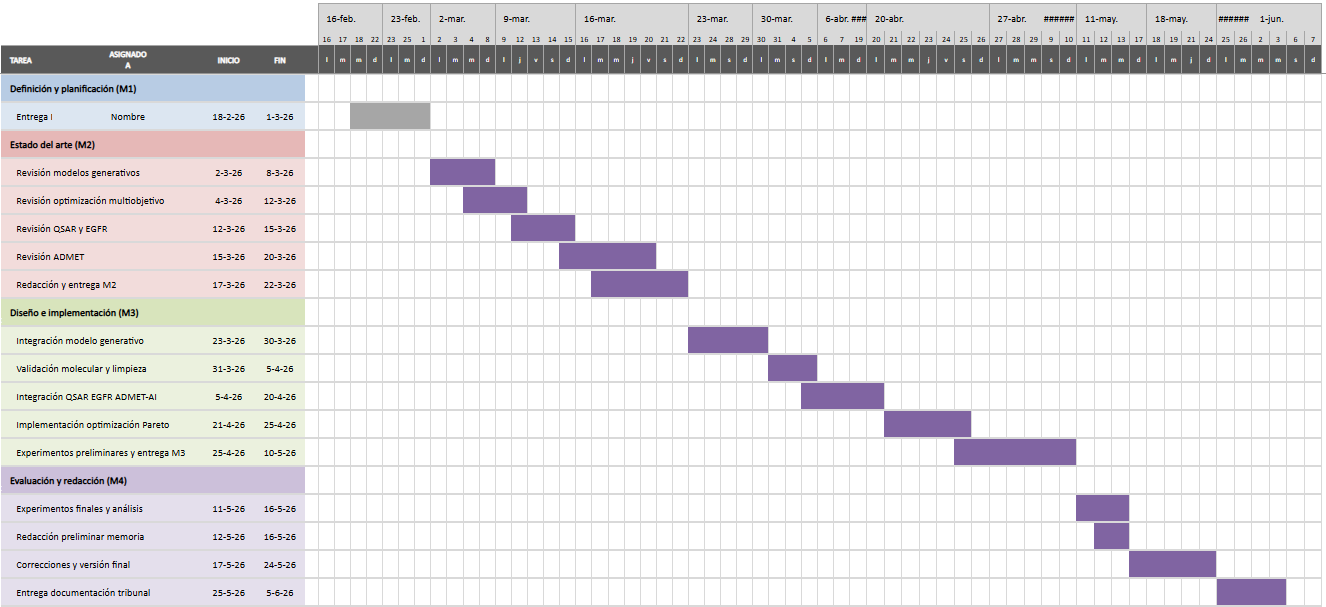
\includegraphics[width=\textwidth]{diagrama_gantt.png}
    \caption{Diagrama de Gantt del proyecto que muestra la planificación temporal de las tareas y fases del trabajo.}
    \label{fig:gantt}
\end{figure}

\subsection{Fase 1: Definición y planificación del proyecto (M1)}

La primera fase se centra en delimitar el problema, definir los objetivos del trabajo y establecer la planificación inicial. En esta etapa también se concreta el alcance del proyecto, diferenciando entre generación molecular, evaluación computacional y priorización de moléculas.

\subsection{Fase 2: Estado del arte (M2)}

La segunda fase consiste en la revisión bibliográfica necesaria para fundamentar el trabajo. Esta revisión incluye modelos generativos moleculares, representación de moléculas mediante SMILES, modelos QSAR como aproximación a la actividad biológica, predicción ADMET y estrategias de optimización multiobjetivo aplicadas al diseño molecular.

\subsection{Fase 3: Diseño e implementación del flujo computacional (M3)}

En esta fase se desarrolla la arquitectura computacional del proyecto. Primero se prepara el conjunto de datos de bioactividad frente a EGFR; después se ajusta el modelo generativo molecular y se generan nuevas estructuras SMILES. Posteriormente se incorporan los procesos de validación química, cálculo de descriptores, predicción de actividad, evaluación ADMET, análisis de similitud estructural y selección multiobjetivo mediante dominancia de Pareto.

\subsection{Fase 4: Evaluación de resultados y redacción final (M4)}

La última fase se dedica al análisis de los resultados obtenidos y a la elaboración de la memoria final. En esta etapa se estudia la calidad de las moléculas generadas, la reducción progresiva del conjunto molecular, el comportamiento del modelo QSAR, el perfil ADMET de las moléculas seleccionadas, la diversidad química y la interpretación crítica del conjunto final.

Paralelamente, se redactan los capítulos finales de la memoria, incluyendo la metodología, los resultados, las conclusiones, las limitaciones del trabajo y las líneas futuras.

\subsection{Riesgos potenciales y planes de mitigación}

Durante el desarrollo del proyecto se identificaron varios riesgos que podían afectar al cumplimiento de la planificación prevista.

\medskip
\textbf{Complejidad técnica en la integración de herramientas.}
\smallskip

La combinación de librerías y modelos diferentes, como RDKit, MRL, scikit-learn y ADMET-AI, podía generar problemas de compatibilidad, instalación o formato de datos. Para mitigar este riesgo, el trabajo se estructuró de forma modular, separando las etapas principales en notebooks independientes y guardando resultados intermedios en disco.

\medskip
\textbf{Coste computacional de los experimentos.}
\smallskip

La generación, validación y evaluación de grandes conjuntos moleculares puede requerir un uso elevado de recursos computacionales. Para reducir este riesgo, se utilizaron tamaños de muestra controlados y se validó el funcionamiento de cada etapa antes de ejecutar procesos más costosos.

\medskip
\textbf{Dependencia de modelos predictivos.}
\smallskip

La interpretación de los resultados depende de modelos computacionales, especialmente el modelo QSAR de actividad y las predicciones ADMET. Estas predicciones no sustituyen a la validación experimental y pueden presentar limitaciones fuera del espacio químico representado en los datos de entrenamiento. Para mitigar este riesgo, los resultados se interpretan como hipótesis moleculares priorizadas y no como candidatos farmacológicos validados.


\section{Breve sumario de productos obtenidos}

Como resultado del trabajo se han obtenido varios productos relacionados con las distintas fases del flujo computacional desarrollado. En primer lugar, se ha construido un conjunto de datos de bioactividad frente a EGFR a partir de registros experimentales de ChEMBL, incluyendo procesos de limpieza, normalización, canonicalización de SMILES y agregación molecular.

A partir de este conjunto se ha ajustado un modelo generativo molecular preentrenado, empleado posteriormente para generar nuevas estructuras químicas representadas como SMILES. Las moléculas generadas han sido validadas, filtradas y evaluadas mediante descriptores fisicoquímicos, predicción de actividad frente a EGFR, propiedades ADMET, métricas de calidad molecular y similitud estructural.

También se ha entrenado un modelo QSAR de regresión para estimar pIC$_{50}$ frente a EGFR, utilizado como señal \textit{proxy} de actividad biológica. De forma complementaria, se han incorporado predicciones ADMET mediante ADMET-AI y se ha aplicado un procedimiento de selección multiobjetivo basado en dominancia de Pareto.

El producto final del proceso es un conjunto reducido de 30 moléculas seleccionadas, acompañado de tablas, métricas y visualizaciones que permiten analizar su actividad predicha, perfil ADMET, calidad molecular, novedad estructural y diversidad química. Además, el trabajo queda organizado en notebooks reproducibles que documentan las fases principales: preprocesado, generación molecular, evaluación y selección, y análisis final de resultados.


\section{Breve descripción de los otros capítulos de la memoria}

La memoria se estructura en varios capítulos que siguen el desarrollo lógico del trabajo realizado.

El \textbf{Capítulo 2} presenta el estado del arte. En él se revisan los conceptos principales relacionados con el descubrimiento computacional de fármacos, la generación molecular mediante inteligencia artificial, la representación de moléculas, los modelos QSAR, la predicción de propiedades ADMET y la optimización multiobjetivo aplicada al diseño molecular.

El \textbf{Capítulo 3} describe los materiales y métodos empleados. Se detallan las fuentes de datos, el preprocesado del conjunto de bioactividad frente a EGFR, el ajuste del modelo generativo, el entrenamiento del modelo QSAR, la evaluación ADMET, el cálculo de descriptores moleculares, el análisis de similitud estructural y el procedimiento de selección mediante dominancia de Pareto.

El \textbf{Capítulo 4} recoge los resultados obtenidos tras ejecutar el flujo computacional completo. Se analiza la calidad de las moléculas generadas, la reducción progresiva del conjunto molecular, el rendimiento del modelo QSAR, la distribución de actividad predicha, el perfil ADMET de las moléculas seleccionadas, su novedad estructural, su diversidad química y los principales riesgos detectados.

El \textbf{Capítulo 5} presenta las conclusiones del trabajo y las líneas futuras. En él se resume el grado de cumplimiento de los objetivos, se interpretan las principales aportaciones metodológicas, se discuten las limitaciones del enfoque y se proponen posibles extensiones, como la incorporación de validación estructural mediante \textit{docking}, análisis más avanzados de sintetizabilidad o modelos generativos condicionados.

\section{Declaración sobre el uso de inteligencia artificial generativa}

Durante la realización de este Trabajo Final de Máster se ha utilizado ChatGPT como herramienta de apoyo puntual para organizar ideas, mejorar la redacción, revisar la coherencia entre apartados y ayudar en la depuración de fragmentos de código.

La inteligencia artificial generativa no se ha utilizado para generar resultados, entrenar modelos, tomar decisiones metodológicas finales ni sustituir el análisis técnico del autor. Los datos, la ejecución de los notebooks, las tablas, las figuras, la interpretación de resultados y las conclusiones son responsabilidad íntegra del autor.

Todas las sugerencias obtenidas mediante esta herramienta han sido revisadas, modificadas y validadas antes de incorporarse al trabajo. Asimismo, ChatGPT no se ha empleado como fuente bibliográfica primaria.

\chapter{Estado del arte}

\section{Descubrimiento de Fármacos Asistido por IA}

El descubrimiento de nuevos fármacos sigue siendo un proceso largo, costoso y con una elevada tasa de fracaso. A diferencia de la industria tecnológica, donde el aumento de capacidad computacional ha reducido costes y acelerado ciclos de desarrollo, el sector farmacéutico se ha enfrentado a una disminución sostenida de productividad conocida como Ley de Eroom [\ref{ref:scannell2012}]. En este contexto, se han descrito costes medios de desarrollo superiores a los 2.600 millones de dólares y tiempos habituales de 10 a 15 años hasta la llegada de un fármaco al mercado [\ref{ref:dimasi2016}].

Una de las razones de esta dificultad es que el descubrimiento farmacológico no consiste únicamente en encontrar una molécula activa frente a una diana. Un candidato debe combinar actividad biológica, propiedades fisicoquímicas compatibles con el uso terapéutico, perfil farmacocinético adecuado y bajo riesgo toxicológico. De hecho, una proporción muy elevada de candidatos fracasa durante el desarrollo clínico, principalmente por falta de eficacia, toxicidad o propiedades ADMET desfavorables [\ref{ref:sun2022},\ref{ref:niazi2025}].

A esta complejidad se suma la magnitud del espacio químico. El número de moléculas potencialmente sintetizables o con propiedades tipo fármaco es tan elevado que el cribado experimental exhaustivo resulta inviable. Por ello, los métodos computacionales se han convertido en herramientas relevantes para explorar, filtrar y priorizar regiones del espacio químico antes de plantear estudios experimentales [\ref{ref:kattuparambil2025}]. Dentro de este marco, la inteligencia artificial permite combinar generación molecular, predicción de propiedades y selección multiobjetivo, que son precisamente los bloques conceptuales sobre los que se apoya este trabajo.

\subsection{Evolución de la computación química}

La computación química ha evolucionado desde métodos clásicos de relación estructura-actividad hacia enfoques más amplios basados en aprendizaje automático y aprendizaje profundo. Tradicionalmente, técnicas como QSAR, docking molecular o dinámica molecular han permitido estimar actividad, afinidad o estabilidad de complejos ligando-proteína. El docking y la dinámica molecular aportan información estructural valiosa, pero requieren una estructura de la diana, una definición razonable del bolsillo de unión y un coste computacional superior al de los modelos ligando-céntricos [\ref{ref:oliveira2025},\ref{ref:niazi2025}].

En paralelo, los modelos de machine learning han permitido aprender patrones a partir de grandes colecciones de moléculas y datos de bioactividad. En lugar de evaluar únicamente compuestos existentes, los modelos generativos permiten proponer nuevas estructuras químicas, mientras que los modelos predictivos ayudan a estimar propiedades relevantes para priorizarlas [\ref{ref:oliveira2025},\ref{ref:zhang2024}]. Este cambio desplaza parte del proceso desde un cribado puramente experimental hacia una etapa previa de exploración computacional, donde se busca reducir el número de hipótesis antes de invertir recursos en validación.

En este trabajo se adopta una aproximación ligando-céntrica basada en SMILES, QSAR, ADMET y selección multiobjetivo. No se pretende reemplazar métodos estructurales como el docking, sino construir una etapa inicial de priorización rápida y reproducible. Esta decisión es coherente con una fase temprana del diseño molecular, en la que el objetivo principal es ordenar y filtrar una muestra amplia de moléculas generadas bajo criterios explícitos.

\section{Parámetros de Calidad Molecular en el Diseño \textit{de novo} de Fármacos}

\subsection{Pequeñas moléculas como modalidad terapéutica}

Las pequeñas moléculas constituyen una modalidad terapéutica especialmente relevante por su tamaño reducido, su posible administración oral, su capacidad para atravesar membranas biológicas y su acceso a dianas intracelulares. Se trata, en general, de compuestos orgánicos de bajo peso molecular cuyas propiedades fisicoquímicas condicionan su absorción, distribución y comportamiento farmacológico [\ref{ref:kattuparambil2025},\ref{ref:niazi2025}].

\begin{figure}[h]
    \centering
    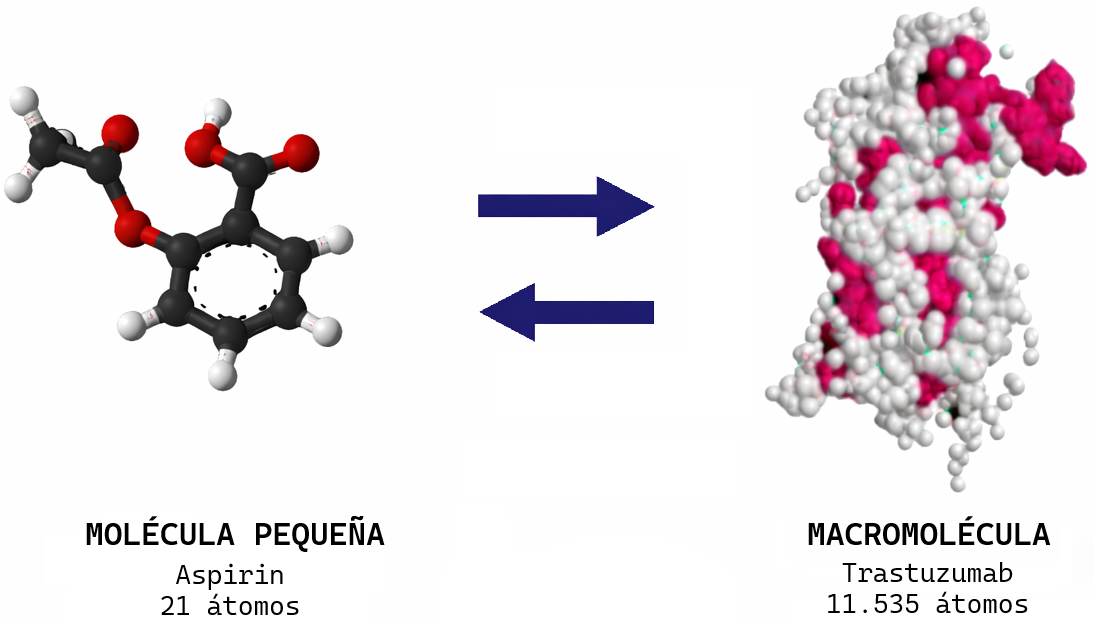
\includegraphics[width=0.75\textwidth]{img/small_vs_large_mol.png}
    \caption{Comparación entre pequeñas moléculas y macromoléculas biológicas.}
    \label{fig:small_vs_large}
\end{figure}

Desde el punto de vista computacional, el interés de las pequeñas moléculas reside en que pueden representarse, generararse y evaluarse mediante descriptores moleculares, huellas estructurales y modelos predictivos. Sin embargo, que una molécula sea pequeña no implica automáticamente que sea adecuada como fármaco. Para que una estructura generada sea una hipótesis razonable debe situarse en rangos fisicoquímicos compatibles con absorción, permeabilidad, solubilidad y estabilidad. Para ello se emplean criterios de \textit{drug-likeness}, como la Regla de Cinco de Lipinski, que relaciona peso molecular, lipofilicidad y capacidad de formar enlaces de hidrógeno con la probabilidad de absorción y permeabilidad oral [\ref{ref:lipinski2001}].

\subsection{Propiedades drug-like y calidad molecular}

La evaluación de la \textit{drug-likeness} permite descartar moléculas con propiedades claramente alejadas de las observadas en fármacos orales conocidos. La Regla de Cinco de Lipinski sigue siendo una referencia clásica porque ofrece una primera aproximación sencilla basada en cuatro propiedades: peso molecular, LogP, donadores de enlaces de hidrógeno y aceptores de enlaces de hidrógeno [\ref{ref:lipinski2001}]. No obstante, estas reglas son filtros aproximados, no garantías de éxito farmacológico.

Para obtener una visión menos binaria se han propuesto métricas continuas como QED (\textit{Quantitative Estimate of Drug-likeness}). QED resume en una puntuación entre 0 y 1 distintas propiedades moleculares asociadas a fármacos conocidos, incluyendo peso molecular, LogP, TPSA, donadores y aceptores de enlace de hidrógeno, enlaces rotables, aromaticidad y alertas estructurales [\ref{ref:bickerton2012},\ref{ref:rdkit}]. En una pipeline generativa, esta métrica permite priorizar moléculas con un perfil global más compatible con compuestos tipo fármaco.

Otra métrica habitual en diseño \textit{de novo} es el \textit{synthetic accessibility score} (SAS), que estima la dificultad de síntesis a partir de contribuciones de fragmentos y penalizaciones de complejidad estructural [\ref{ref:ertl2009}]. Su interpretación es inversa a QED: valores bajos indican estructuras más accesibles y valores altos indican mayor complejidad sintética. Aunque SAS es muy relevante para etapas posteriores, en este trabajo no se incorpora como variable calculada en la pipeline. Por tanto, debe entenderse como una limitación metodológica y una posible extensión futura, no como un criterio usado en la selección final.

En conjunto, la calidad molecular no debe interpretarse como una única propiedad, sino como un equilibrio entre tamaño, lipofilicidad, polaridad, flexibilidad, capacidad de interacción y ausencia de alertas estructurales graves. Esta idea justifica que el trabajo combine filtros fisicoquímicos, QED, reglas tipo Lipinski, predicciones ADMET y similitud estructural en lugar de depender de una sola métrica.

\subsubsection{Perfil ADMET}

La actividad frente a una diana terapéutica no es suficiente para considerar prometedora una molécula. Un candidato debe mostrar propiedades adecuadas de absorción, distribución, metabolismo, excreción y toxicidad (ADMET). Estas dimensiones condicionan si el compuesto puede alcanzar concentraciones eficaces en el organismo sin producir riesgos inaceptables de toxicidad [\ref{ref:sun2022},\ref{ref:niazi2025}].

La predicción ADMET temprana es especialmente importante en diseño molecular generativo porque los modelos pueden producir estructuras químicamente válidas pero con perfiles farmacocinéticos o toxicológicos poco realistas. Herramientas modernas como ADMET-AI permiten estimar múltiples \textit{endpoints} de forma automatizada, incluyendo propiedades relacionadas con absorción intestinal, biodisponibilidad, permeabilidad, metabolismo por enzimas CYP, cardiotoxicidad asociada a hERG, mutagenicidad AMES, toxicidad clínica, carcinogenicidad y alertas estructurales [\ref{ref:swanson2024},\ref{ref:admet_ai_web},\ref{ref:admet_ai_github}].

En una fase temprana de priorización, estas predicciones no deben interpretarse como evidencia definitiva de seguridad, sino como señales de riesgo. Por este motivo, resulta útil separar criterios ADMET duros, asociados a alertas críticas, de puntuaciones blandas que permiten ordenar moléculas con perfiles intermedios. Esta distinción evita que un riesgo toxicológico relevante quede diluido dentro de una media global aparentemente favorable [\ref{ref:swanson2024}].

\subsection{EGFR como diana terapéutica}

El receptor del factor de crecimiento epidérmico (EGFR) es una proteína transmembrana con actividad tirosina quinasa implicada en proliferación, supervivencia celular y señalización oncogénica. Su activación anómala o sobreexpresión se ha relacionado con distintos tumores sólidos, especialmente con el cáncer de pulmón de células no pequeñas (NSCLC), donde los inhibidores de EGFR han tenido un papel terapéutico relevante [\ref{ref:nada2023}].

\begin{figure}[h]
    \centering
    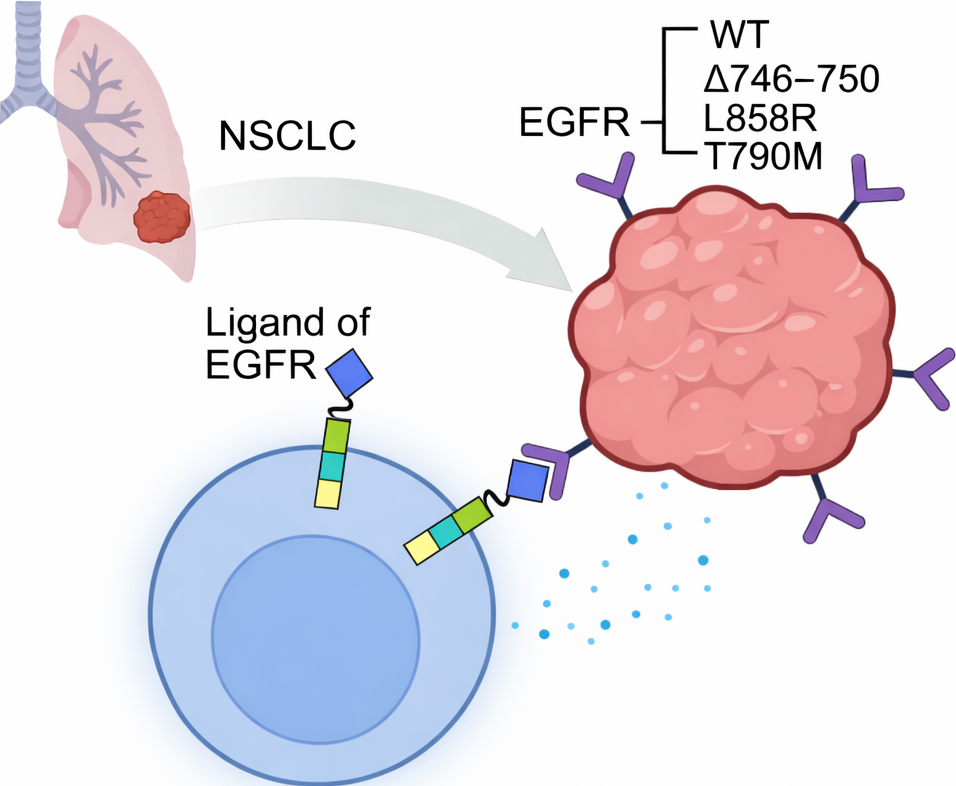
\includegraphics[width=0.55\textwidth]{img/egfr_photo.png}
    \caption{Esquema de la vía de señalización del EGFR y sus principales mutaciones en el cáncer de pulmón de células no pequeñas (NSCLC).}
    \label{fig:egfr_nsclc}
\end{figure}

A pesar del éxito clínico de varios inhibidores de tirosina quinasa, la aparición de mutaciones de resistencia limita su eficacia. Mutaciones como T790M pueden reducir la unión de inhibidores de primera y segunda generación, mientras que C797S se asocia con resistencia a inhibidores de tercera generación. Este escenario mantiene el interés por explorar nuevas entidades químicas relacionadas con EGFR [\ref{ref:nada2023}].

Desde el punto de vista químico, una molécula \textit{EGFR-like} plausible no debería evaluarse solo por su actividad predicha. También debería presentar un peso molecular moderado, lipofilicidad controlada, polaridad compatible con permeabilidad, número razonable de donadores y aceptores de hidrógeno, y ausencia de alertas toxicológicas evidentes. Además, en química médica es importante analizar el \textit{scaffold} o núcleo estructural de una molécula, ya que pequeñas modificaciones sobre un mismo scaffold pueden generar familias de análogos con propiedades similares. Los scaffolds de Murcko ofrecen una forma simplificada de representar ese núcleo molecular y permiten estudiar diversidad estructural dentro de un conjunto de candidatos [\ref{ref:bemis1996}].

\section{Representación Computacional de Moléculas y Proteínas}

La representación computacional determina qué información química puede aprender un modelo. En descubrimiento molecular se utilizan representaciones lineales, como SMILES, representaciones basadas en grafos y representaciones tridimensionales o dependientes de la proteína. Cada una captura aspectos distintos de la molécula y condiciona tanto la generación como la predicción de propiedades [\ref{ref:zhang2024},\ref{ref:oliveira2025}].

\subsection{Representación lineal mediante SMILES}

El sistema SMILES (\textit{Simplified Molecular Input Line Entry System}) codifica moléculas como cadenas de caracteres que representan átomos, enlaces, ramificaciones y ciclos [\ref{ref:weininger1988}]. Formalmente, una molécula puede representarse como una secuencia:

\begin{equation}
S = (s_1, s_2, \dots, s_n), \quad s_i \in \mathcal{V}
\end{equation}

donde $\mathcal{V}$ es el vocabulario de símbolos químicos.

Por ejemplo, la molécula de etanol puede representarse como:

\begin{equation}
\texttt{CCO}
\end{equation}

Esta notación permite tratar las moléculas como texto y facilita el uso de modelos generativos secuenciales, como redes recurrentes o modelos de lenguaje. Su principal ventaja es la simplicidad: millones de moléculas pueden almacenarse y procesarse como secuencias. Su principal limitación es que no representa explícitamente la geometría tridimensional, por lo que no captura directamente interacciones espaciales con una proteína [\ref{ref:weininger1988},\ref{ref:zhang2024}].

En este trabajo, SMILES es la representación central porque el modelo generativo empleado genera secuencias moleculares y las etapas posteriores de validación, canonicalización y cálculo de descriptores se realizan a partir de dichas cadenas.

\subsection{Representación basada en grafos moleculares}

Una molécula también puede representarse como un grafo, donde los átomos son nodos y los enlaces son aristas. Formalmente, una molécula puede definirse como [\ref{ref:oliveira2025}]:

\begin{equation}
G = (V, E)
\end{equation}

donde $V$ es el conjunto de nodos y $E$ el conjunto de aristas. Cada nodo puede contener información como tipo de átomo, carga o hibridación, y cada arista puede describir el tipo de enlace. Esta representación es especialmente adecuada para redes neuronales de grafos y para modelos que buscan aprender directamente la estructura molecular. Aunque el generador de este trabajo opera con SMILES, los fingerprints y varios modelos de predicción pueden interpretarse como formas comprimidas de capturar patrones estructurales derivados del grafo molecular.


\section{Modelado predictivo de propiedades moleculares}

La generación molecular solo produce hipótesis estructurales. Para priorizarlas es necesario estimar propiedades asociadas a actividad, calidad molecular y seguridad. Por ello, las pipelines modernas de diseño molecular combinan modelos generativos con modelos predictivos y reglas de filtrado [\ref{ref:niazi2025},\ref{ref:oliveira2025}].

\subsection{Modelos QSAR en descubrimiento de fármacos}

Los modelos QSAR (\textit{Quantitative Structure--Activity Relationship}) relacionan la estructura de una molécula con una propiedad biológica de interés. Para ello, las moléculas se transforman en descriptores, fingerprints o representaciones aprendidas que sirven como entrada a modelos supervisados [\ref{ref:rogers2010},\ref{ref:breiman2001}].

En fases tempranas de cribado virtual, los modelos QSAR permiten evaluar grandes bibliotecas de compuestos con un coste computacional bajo. Pueden formularse como modelos de clasificación, por ejemplo para distinguir activos e inactivos, o como modelos de regresión, por ejemplo para predecir IC$_{50}$, K$_i$ o pIC$_{50}$. Esta flexibilidad los hace adecuados para integrarse en flujos generativos donde se necesita una señal rápida de actividad [\ref{ref:nada2023},\ref{ref:pham2025}].

\subsubsection{QSAR como aproximación a la afinidad frente a una diana}

En el diseño molecular asistido por IA, la afinidad real frente a una diana no puede conocerse sin ensayos experimentales. Por ello, un modelo QSAR entrenado con datos experimentales de una diana concreta puede utilizarse como señal \textit{proxy} para ordenar moléculas candidatas [\ref{ref:nada2023}]. En este trabajo, la pIC$_{50}$ predicha frente a EGFR cumple precisamente esa función: no valida actividad biológica real, pero permite priorizar moléculas que se parecen, en términos de patrones estructurales, a compuestos con actividad experimental conocida.

La principal limitación de los modelos QSAR es su dominio de aplicabilidad. Un modelo puede funcionar razonablemente bien para moléculas similares a las usadas durante su entrenamiento, pero perder fiabilidad al extrapolar hacia regiones químicas alejadas. Por ello, conviene interpretar sus predicciones junto con medidas de similitud estructural, diversidad de scaffolds y controles de novedad. Además, pequeñas diferencias de pIC$_{50}$ predicha no deben sobreinterpretarse como diferencias reales de potencia experimental [\ref{ref:niazi2025}].

\begin{figure}[H]
    \centering
    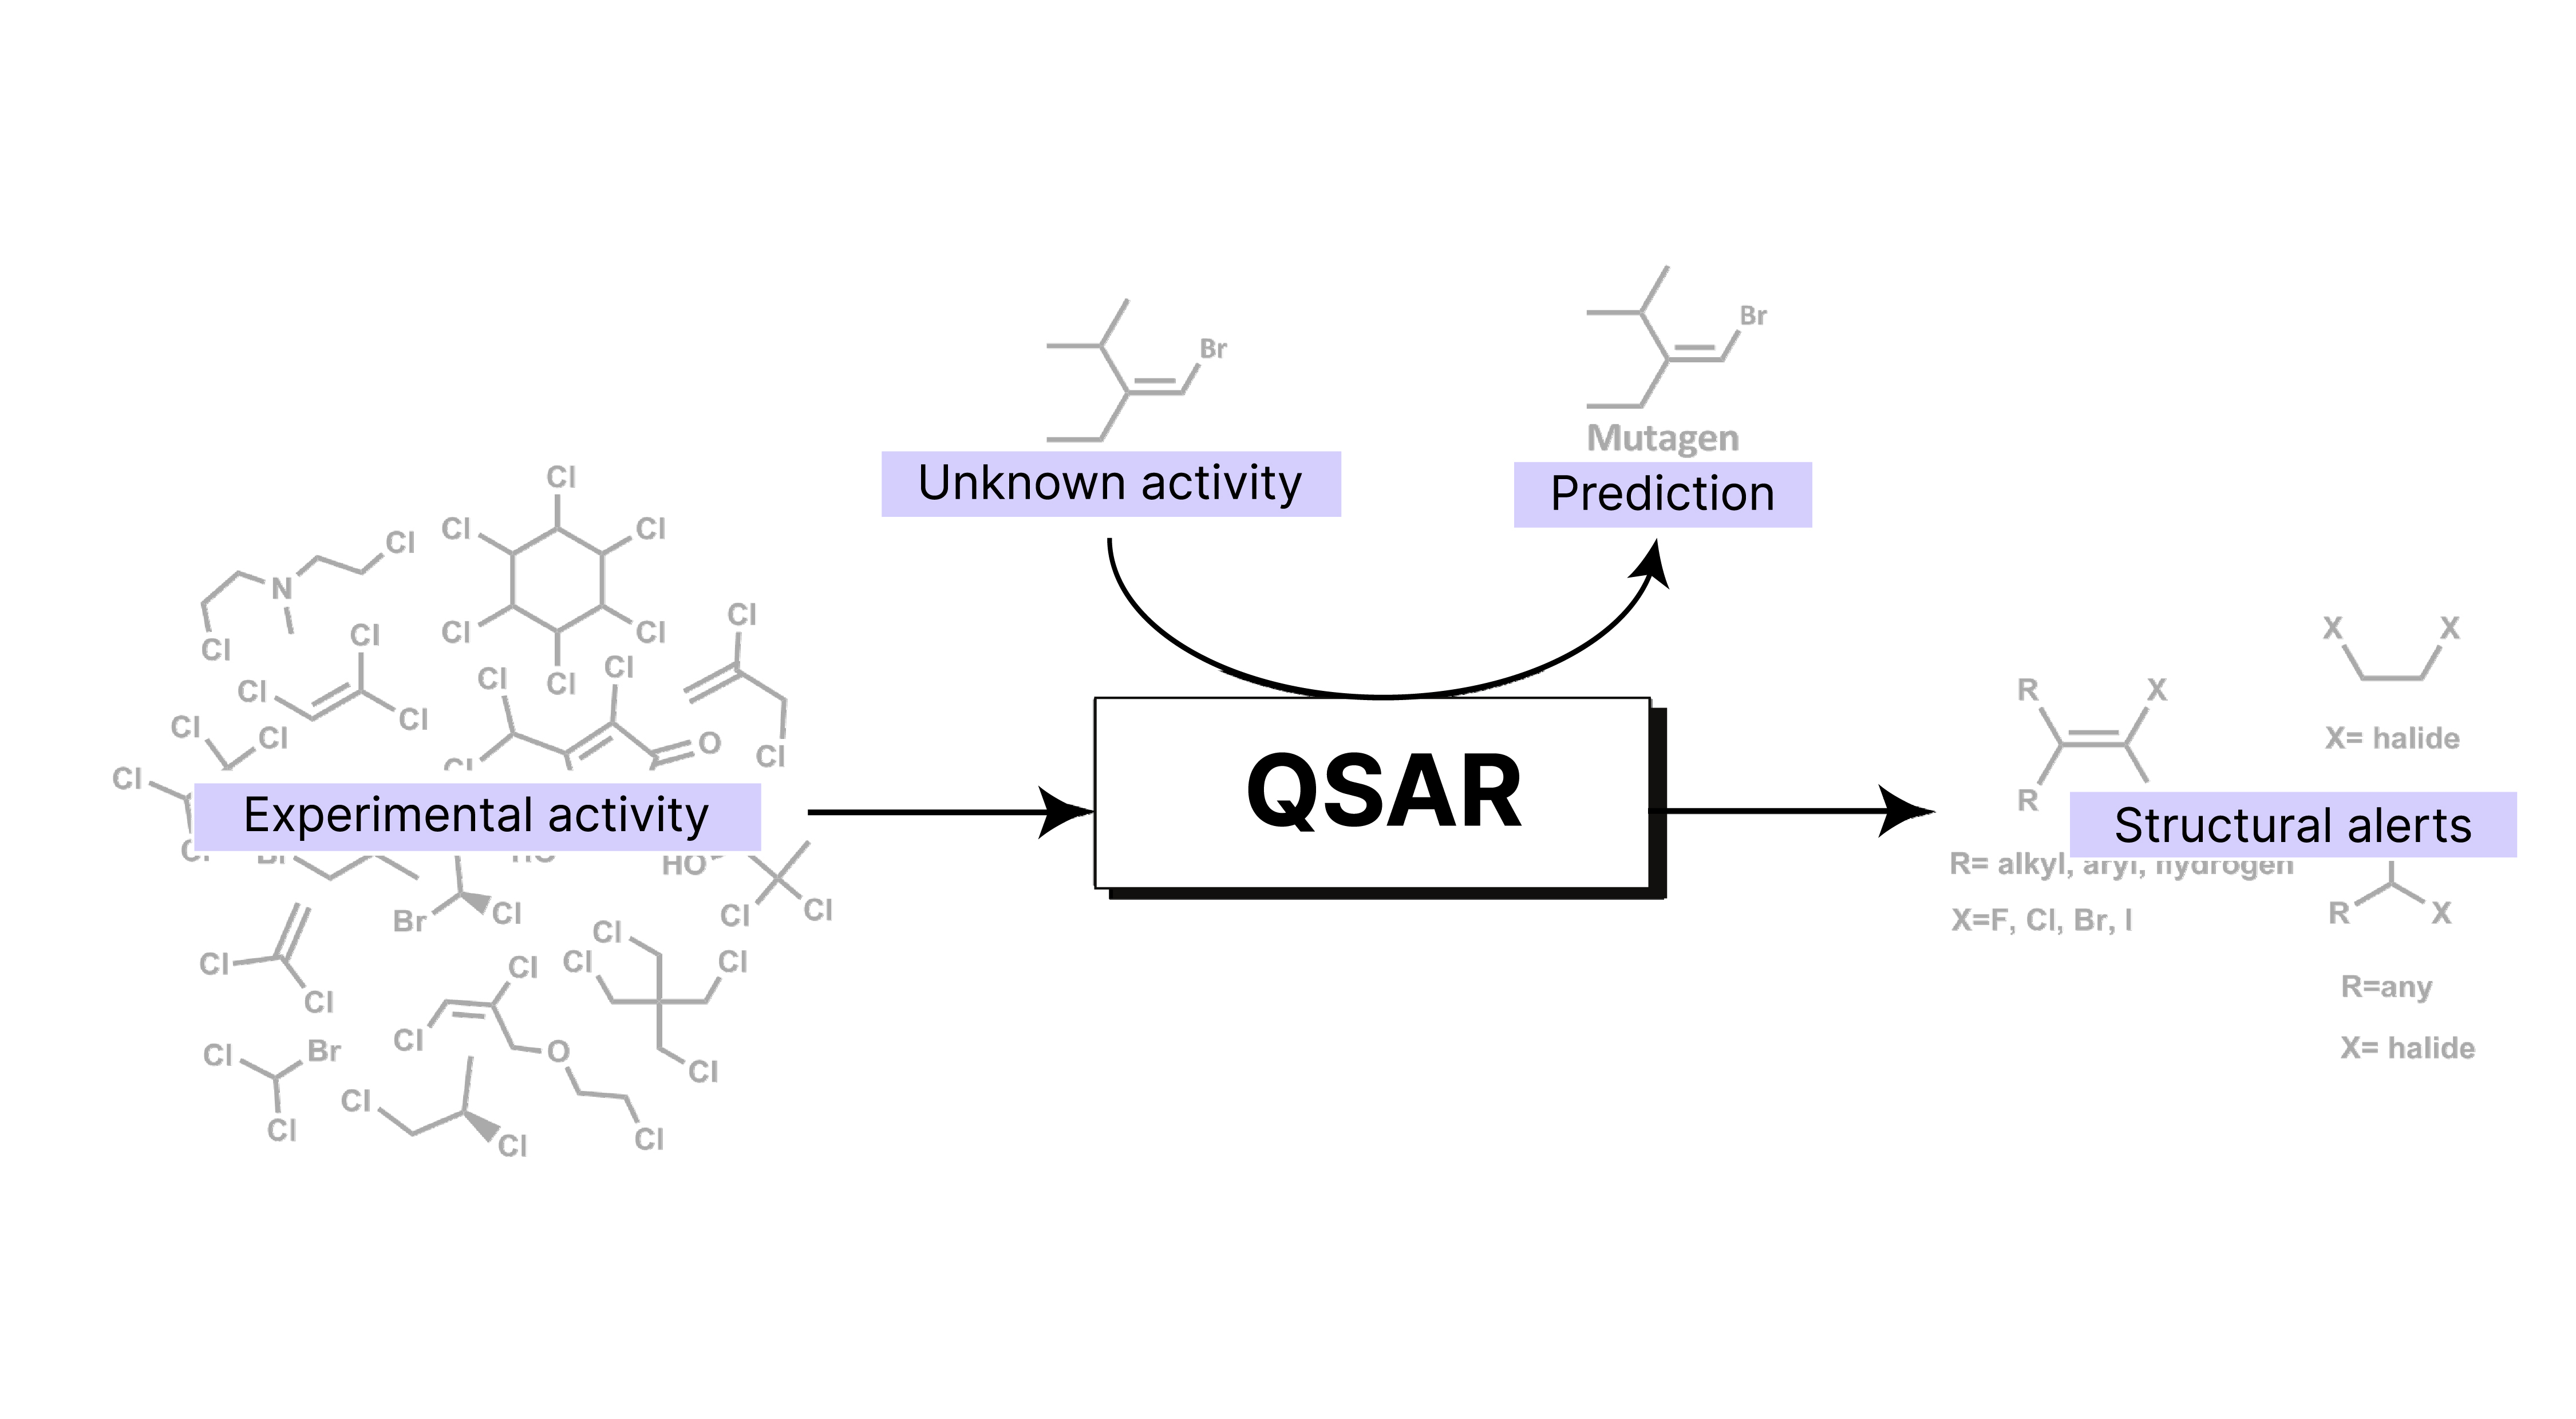
\includegraphics[width=0.75\textwidth]{img/qsar_diagram.jpg}
    \caption{Esquema general de un modelo QSAR: a partir de datos de actividad experimental se generan predicciones y alertas estructurales.}
    \label{fig:qsar}
\end{figure}

\subsection{Predicción computacional de propiedades ADMET}

Además de la actividad frente a EGFR, una molécula candidata debe presentar un perfil ADMET razonable. La predicción computacional de propiedades ADMET estima, a partir de la estructura química, señales relacionadas con absorción intestinal, biodisponibilidad, distribución, metabolismo, eliminación y toxicidad [\ref{ref:sun2022},\ref{ref:swanson2024}].

A diferencia de la actividad frente a una diana, ADMET es un problema multidimensional. Una molécula puede ser favorable en absorción pero desfavorable en toxicidad, o mostrar buen perfil general pero riesgo de interacción con canales hERG. Por tanto, la evaluación ADMET encaja de forma natural con enfoques multiobjetivo, donde el objetivo no es maximizar una única propiedad sino equilibrar riesgos y beneficios [\ref{ref:swanson2024},\ref{ref:angelo2023}].

\subsubsection{Herramientas modernas de predicción ADMET basadas en IA}

ADMET-AI es una plataforma de predicción basada en aprendizaje automático diseñada para evaluar bibliotecas químicas de gran tamaño. Proporciona predicciones para múltiples endpoints y puede utilizarse como herramienta web o mediante ejecución local, lo que facilita su integración en pipelines reproducibles [\ref{ref:swanson2024},\ref{ref:admet_ai_web},\ref{ref:admet_ai_github}].

En el contexto de este TFM, ADMET-AI es relevante no solo por generar predicciones individuales, sino porque permite construir criterios de filtrado y puntuaciones agregadas. En particular, endpoints como AMES, ClinTox, carcinogenicidad, hERG, biodisponibilidad e HIA pueden utilizarse como señales tempranas para descartar perfiles problemáticos o penalizarlos durante la priorización.

\section{Modelos generativos moleculares}

Los modelos generativos moleculares aprenden patrones a partir de conjuntos de moléculas y los utilizan para proponer nuevas estructuras. A diferencia del cribado virtual clásico, que evalúa moléculas ya existentes en una biblioteca, la generación \textit{de novo} permite explorar regiones no cubiertas explícitamente por el conjunto inicial [\ref{ref:kattuparambil2025},\ref{ref:oliveira2025},\ref{ref:angelo2023}].

\subsection{Generación molecular \textit{de novo}}

La generación molecular \textit{de novo} consiste en diseñar nuevas entidades químicas a partir de una distribución aprendida. Formalmente, dado un conjunto de moléculas de entrenamiento $\mathcal{D} = \{x_1, x_2, \dots, x_n\}$, un modelo generativo aprende una distribución $p(x)$ sobre el espacio molecular, de modo que nuevas muestras $\tilde{x} \sim p(x)$ correspondan a estructuras químicamente plausibles.

Este planteamiento permite pasar de una exploración pasiva del espacio químico a una generación activa de hipótesis. Sin embargo, generar moléculas válidas no garantiza que sean activas, seguras o desarrollables. Por ello, la generación debe acompañarse de validación química, cálculo de propiedades, evaluación ADMET y selección posterior [\ref{ref:angelo2023},\ref{ref:olivecrona2017}].

\subsection{Modelos generativos modernos}

Existen distintas familias de modelos generativos moleculares. Los modelos secuenciales autoregresivos generan SMILES carácter a carácter o token a token, aprendiendo la sintaxis química como si fuera un lenguaje. En esta familia se sitúan modelos basados en redes recurrentes, como LSTM, que han sido ampliamente utilizados en generación molecular y pueden adaptarse mediante fine-tuning o aprendizaje por refuerzo [\ref{ref:olivecrona2017}].

Más recientemente, los modelos basados en Transformers han ganado relevancia por su capacidad para capturar dependencias globales en secuencias moleculares. También existen modelos basados en grafos, que generan directamente estructuras moleculares como nodos y aristas, y modelos de difusión, especialmente prometedores para generación tridimensional y tareas donde la geometría molecular es importante [\ref{ref:zhang2024},\ref{ref:oliveira2025}].

La elección del modelo depende del objetivo del trabajo. En este TFM se utiliza un modelo LSTM preentrenado de la librería MRL, por lo que la generación se formula como un problema de lenguaje molecular sobre SMILES. Esto permite un flujo sencillo y reproducible, aunque no incorpora de forma directa condiciones sobre EGFR, ADMET o geometría 3D.

\subsection{Modelos preentrenados en química molecular}

El preentrenamiento molecular consiste en entrenar modelos sobre grandes colecciones químicas, como ZINC, ChEMBL o PubChem, para capturar regularidades generales del espacio molecular [\ref{ref:zhang2024},\ref{ref:zdrazil2024}]. Posteriormente, el modelo puede ajustarse a un dominio específico mediante fine-tuning, reduciendo el coste de entrenamiento y aprovechando conocimiento químico previo.

En este trabajo, esta lógica se aplica mediante el uso de un modelo generativo molecular preentrenado de MRL, ajustado sobre moléculas activas frente a EGFR [\ref{ref:mrl_docs},\ref{ref:mrl_tutorial_affinity}]. Es importante subrayar que el modelo empleado no es condicional: no recibe como entrada una proteína, una actividad deseada ni un vector de propiedades. Por ello, la optimización no ocurre durante la generación, sino después, mediante scoring, filtros y selección multiobjetivo.

\section{Optimización multiobjetivo en diseño molecular}

El diseño molecular es un problema multiobjetivo porque una molécula debe equilibrar actividad, propiedades fisicoquímicas, ADMET, novedad y plausibilidad química. Optimizar una sola dimensión puede producir candidatos desequilibrados: moléculas muy activas pero tóxicas, muy novedosas pero fuera del dominio del modelo, o muy drug-like pero poco relevantes para la diana [\ref{ref:angelo2023},\ref{ref:deb2002}].

Las propiedades relevantes de una molécula no siempre están alineadas. Por ejemplo, aumentar la afinidad puede ir acompañado de mayor lipofilicidad, lo que puede empeorar solubilidad o toxicidad. Del mismo modo, estructuras complejas pueden presentar actividad favorable pero ser difíciles de sintetizar [\ref{ref:angelo2023},\ref{ref:ertl2009}].

Este tipo de relaciones introduce tensiones entre objetivos, que pueden representarse de forma general como:

\begin{equation}
\max \; f_1(x), \quad \max \; f_2(x), \quad \dots, \quad \min \; f_k(x)
\end{equation}

donde cada función $f_i(x)$ representa una propiedad relevante del compuesto $x$. En este marco, no se busca necesariamente una única molécula óptima, sino un conjunto de soluciones que representen compromisos razonables entre criterios [\ref{ref:angelo2023},\ref{ref:deb2002}].

\subsection{Estrategias de optimización molecular}

Una estrategia habitual consiste en combinar múltiples objetivos mediante una función escalar ponderada:

\begin{equation}
F(x) = \sum_{i=1}^{k} w_i f_i(x)
\end{equation}

donde $w_i$ representa el peso asignado a cada objetivo. Este enfoque es fácil de interpretar, pero obliga a decidir de antemano cuánto pesa cada propiedad y puede ocultar soluciones interesantes que destacan en un objetivo concreto [\ref{ref:angelo2023}].

Otra estrategia consiste en modificar directamente el proceso generativo mediante aprendizaje por refuerzo o modelos condicionados. En estos casos, el generador aprende a producir moléculas que maximizan una función de recompensa. Aunque este enfoque puede ser potente, también puede reducir diversidad o favorecer soluciones que explotan debilidades de la función objetivo si no se controla adecuadamente [\ref{ref:olivecrona2017},\ref{ref:angelo2023}].

El presente trabajo adopta una estrategia más modular: primero genera moléculas con un modelo no condicional y después las evalúa mediante una fase de scoring y selección. Esta separación facilita auditar cada criterio por separado y evita que el comportamiento del generador quede mezclado con las decisiones de priorización.

\subsection{Dominancia de Pareto y soluciones no dominadas}

La dominancia de Pareto permite seleccionar soluciones competitivas sin reducir todos los objetivos a una única puntuación. Una solución $x_1$ domina a otra solución $x_2$ si es al menos tan buena en todos los objetivos y estrictamente mejor en al menos uno:

\begin{equation}
x_1 \prec x_2 \iff \forall i, \; f_i(x_1) \geq f_i(x_2) \;\; \text{y} \;\; \exists j \; \text{tal que} \; f_j(x_1) > f_j(x_2)
\end{equation}

El conjunto de soluciones no dominadas constituye el frente de Pareto. En estas soluciones no es posible mejorar un objetivo sin empeorar al menos otro, por lo que representan compromisos útiles para la toma de decisiones [\ref{ref:deb2002},\ref{ref:angelo2023}].

\begin{figure}[h]
    \centering
    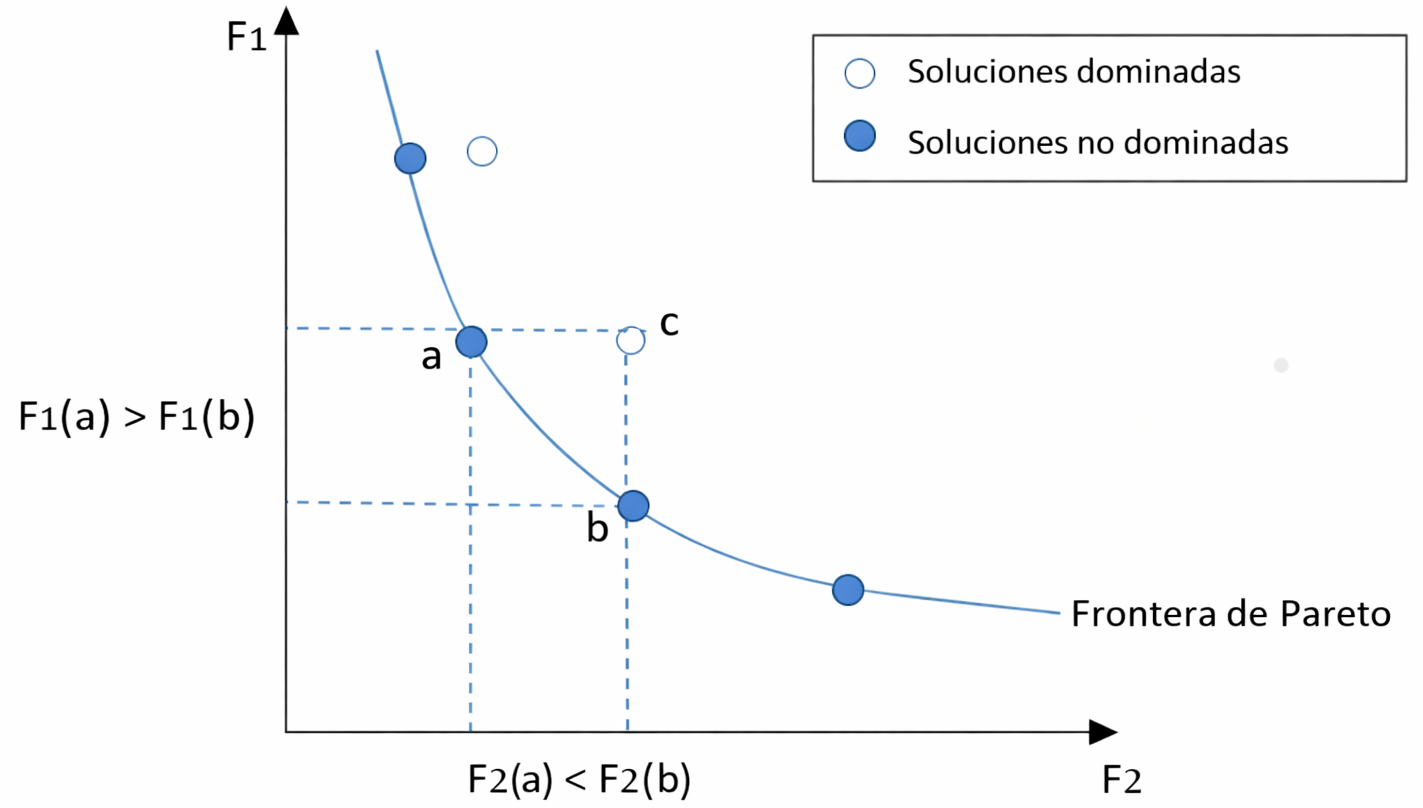
\includegraphics[width=0.7\linewidth]{img/funcion_frontera_pareto.png}
    \caption{Ejemplo de frente de Pareto en un problema multiobjetivo.}
    \label{fig:pareto}
\end{figure}

En la Figura~\ref{fig:pareto}, las soluciones situadas en el frente no dominado representan alternativas con distintos equilibrios entre objetivos. Las soluciones dominadas, en cambio, pueden descartarse porque existe al menos otra alternativa igual o mejor en todos los criterios considerados.

\subsection{Métricas de evaluación multiobjetivo}

Además de identificar soluciones no dominadas, existen métricas para evaluar la calidad global de un frente de Pareto. El hipervolumen mide el volumen del espacio de objetivos dominado por el conjunto de soluciones respecto a un punto de referencia, mientras que la dispersión o \textit{spread} evalúa cómo se distribuyen las soluciones a lo largo del frente [\ref{ref:angelo2023},\ref{ref:deb2002}].

En este trabajo estas métricas se consideran como contexto metodológico, pero no se utilizan como criterio principal de selección. La selección se basa en dominancia de Pareto y, posteriormente, en una puntuación ponderada auxiliar para ordenar soluciones no dominadas. Esta decisión mantiene la interpretación multiobjetivo sin renunciar a una herramienta práctica de ranking.

\subsubsection{Hipervolumen (\textit{Hypervolume})}

El hipervolumen cuantifica cuánto espacio favorable cubre un conjunto de soluciones no dominadas respecto a un punto de referencia. En diseño molecular puede ser útil para comparar algoritmos generativos, aunque requiere definir cuidadosamente los objetivos, escalas y punto de referencia.

\subsubsection{Dispersión (\textit{Spread})}

La dispersión mide si las soluciones se concentran en una zona concreta del frente o si cubren distintos compromisos. En una shortlist molecular, una mayor diversidad de perfiles puede ser útil porque evita seleccionar únicamente moléculas muy parecidas entre sí.

\subsubsection{Número de soluciones no dominadas}

El número de soluciones no dominadas ofrece una medida simple del tamaño del frente de Pareto. No obstante, un frente grande no implica necesariamente mejor calidad: también debe evaluarse si las soluciones son interpretables, diversas y químicamente plausibles.

\subsubsection{Funciones agregadas (DScore)}

Algunos enfoques combinan objetivos en una puntuación agregada:

\begin{equation}
D(x) = \sum_{i=1}^{k} w_i f_i(x)
\end{equation}

Este tipo de función facilita ordenar moléculas, pero introduce arbitrariedad en los pesos. Por ello, en este trabajo se utiliza solo como apoyo interpretativo tras aplicar criterios mínimos de elegibilidad y selección por Pareto.




\chapter{Materiales y métodos}

El presente capítulo describe la metodología seguida para desarrollar la \textit{pipeline} computacional propuesta. El trabajo se estructuró como una investigación aplicada e incremental: primero se preparó un conjunto de datos fiable de actividad frente a EGFR, después se adaptó un modelo generativo molecular preentrenado, posteriormente se evaluaron las moléculas generadas mediante criterios de actividad, propiedades fisicoquímicas, ADMET y similitud estructural, y finalmente se aplicó una selección multiobjetivo basada en dominancia de Pareto.

La decisión metodológica central fue no entrenar todos los componentes desde cero, sino integrar herramientas y modelos especializados dentro de un flujo reproducible. Esta elección es coherente con el objetivo del trabajo: diseñar y evaluar una arquitectura de inteligencia artificial aplicada al descubrimiento molecular, más que proponer un nuevo algoritmo generativo o un nuevo modelo QSAR. Por ello, cada fase de la \textit{pipeline} se diseñó como un bloque independiente, con entradas y salidas persistidas en disco, permitiendo auditar los resultados intermedios y repetir el proceso completo de forma controlada.

\section{Diseño general de la metodología}

La metodología se dividió en cuatro etapas principales, implementadas en notebooks independientes:

\begin{itemize}
    \item \textbf{Preprocesado del dataset de bioactividad}: limpieza, normalización, canonicalización y agregación de datos experimentales de IC50 frente a EGFR.
    \item \textbf{Fine-tuning y generación molecular}: adaptación de un modelo generativo preentrenado de SMILES al espacio químico de moléculas activas frente a EGFR.
    \item \textbf{Scoring y selección multiobjetivo}: cálculo de descriptores, entrenamiento de un modelo QSAR, predicción de pIC50, integración de ADMET-AI, cálculo de similitudes estructurales y selección mediante Pareto.
    \item \textbf{Análisis posterior de candidatas}: interpretación de la shortlist final desde diferentes perfiles: actividad, ADMET, novedad, diversidad estructural y equilibrio global.
\end{itemize}

Esta separación evita mezclar objetivos metodológicos distintos. El modelo generativo aprende una distribución de secuencias SMILES; los descriptores fisicoquímicos, las predicciones de actividad y las restricciones ADMET pertenecen a la fase posterior de evaluación. Incluir estas variables directamente en el entrenamiento del LSTM no aportaría información útil, ya que el modelo empleado no es condicional. Por tanto, la optimización se realiza \textit{post-generación}, mediante scoring y selección multiobjetivo.

\begin{table}[H]
    \centering
    \small
    \begin{tabular}{p{4.2cm} p{5.1cm} p{4.7cm}}
        \hline
        \textbf{Notebook} & \textbf{Función principal} & \textbf{Salida principal} \\
        \hline
        \texttt{01\_preprocesado} & Limpieza y agregación del dataset de IC50 frente a EGFR. & \texttt{model\_preprocesed\_dataset.csv} y \texttt{model\_procesed\_dataset.csv}. \\
        \hline
        \texttt{02\_SMILES\_generation} & Fine-tuning del modelo MRL y generación de moléculas nuevas. & \texttt{generated\_molecules.csv}. \\
        \hline
        \texttt{03\_scoring} & Scoring, ADMET, similitud, Pareto y shortlist final. & \texttt{shortlist30\_final\_candidates.csv}. \\
        \hline
        \texttt{04\_conclusiones} & Análisis interpretativo de candidatas y generación de figuras de apoyo. & Tablas, rankings y visualizaciones para discusión de resultados. \\
        \hline
    \end{tabular}
    \caption{Estructura modular de los notebooks empleados en el desarrollo de la pipeline.}
    \label{tab:notebooks_pipeline}
\end{table}

\section{Materiales, entorno y librerías empleadas}

El desarrollo se realizó en Python, utilizando notebooks de Jupyter como entorno principal de experimentación. La elección de notebooks se justifica por su utilidad en proyectos exploratorios de ciencia de datos, ya que permiten combinar código, resultados intermedios, visualizaciones y justificación metodológica en un mismo documento ejecutable.

Las principales librerías empleadas fueron:

\begin{itemize}
    \item \textbf{RDKit}: validación y canonicalización de SMILES, cálculo de descriptores fisicoquímicos, fingerprints Morgan, coeficientes de Tanimoto y scaffolds de Murcko [\ref{ref:rdkit},\ref{ref:bemis1996}].
    \item \textbf{MRL}: carga del modelo molecular generativo preentrenado y fine-tuning supervisado sobre SMILES activos frente a EGFR [\ref{ref:mrl_docs},\ref{ref:mrl_tutorial_affinity}].
    \item \textbf{PyTorch}: backend de entrenamiento del modelo generativo.
    \item \textbf{scikit-learn}: entrenamiento del modelo QSAR basado en Random Forest y cálculo de métricas de regresión [\ref{ref:pedregosa2011}].
    \item \textbf{ADMET-AI}: predicción de propiedades farmacocinéticas y toxicológicas de las moléculas generadas [\ref{ref:swanson2024}].
    \item \textbf{pandas, numpy y matplotlib}: manipulación de datos, análisis numérico y visualización.
\end{itemize}

Para garantizar reproducibilidad, se fijó una semilla común de aleatoriedad igual a \textbf{42} en las fases de generación, particionado de datos y entrenamiento del modelo predictivo. Además, cada fase generó archivos intermedios en carpetas diferenciadas, separando datos, modelos, resultados finales y resúmenes de ejecución.

\section{Preprocesado del dataset de bioactividad EGFR}

\subsection{Datos de entrada y exportación desde ChEMBL}

La primera etapa del trabajo consistió en construir un dataset de bioactividad específico para EGFR a partir de datos experimentales procedentes de ChEMBL [\ref{ref:zdrazil2024}]. La descarga se realizó directamente desde el explorador de actividades de ChEMBL, disponible en:

\vspace{0.1cm}
\begin{center}
\url{https://www.ebi.ac.uk/chembl/explore/activities/}
\end{center}
\vspace{0.1cm}

Antes de exportar el archivo CSV, se aplicaron filtros en la propia interfaz web con el objetivo de restringir el conjunto inicial a registros relevantes para el caso de estudio.

En primer lugar, se utilizó el filtro personalizado \texttt{target\_chembl\_id:CHEMBL203}, correspondiente a la diana EGFR humana. Posteriormente, mediante los filtros interactivos de ChEMBL, se restringieron las actividades a:

\begin{itemize}
    \item \texttt{Standard Type = IC50}, para conservar únicamente medidas de concentración inhibitoria media;
    \item \texttt{Target Organism = Homo sapiens}, para evitar mezclar datos procedentes de organismos distintos.
\end{itemize}

La aplicación de estos filtros previos generó el archivo \texttt{egfr\_activity\_IC50.csv}, que fue empleado como entrada del notebook \texttt{01\_preprocesado.ipynb}. El archivo bruto contenía inicialmente 25.758 registros y 48 columnas. Esta exportación no se utilizó directamente para entrenar modelos, ya que todavía incluía columnas no necesarias, registros con unidades no homogéneas, relaciones experimentales censuradas y valores potencialmente problemáticos desde el punto de vista de validez experimental.

\subsection{Datos de entrada}

La primera etapa partió de un dataset bruto de actividad frente a EGFR en formato CSV, almacenado como \texttt{egfr\_activity\_IC50.csv}. El archivo contenía inicialmente 25.758 registros y 48 columnas. Tras eliminar columnas no necesarias para el objetivo del trabajo, el dataset quedó reducido a 21 columnas de interés.

El preprocesado se centró exclusivamente en medidas comparables de IC50 frente a EGFR. Para ello se aplicaron los siguientes criterios:

\begin{itemize}
    \item diana igual a \texttt{CHEMBL203}, correspondiente a EGFR;
    \item tipo de medida igual a \texttt{IC50};
    \item unidades normalizadas a nanomolar, \texttt{nM};
    \item valores de actividad positivos;
    \item relación experimental exacta, \texttt{Standard Relation = ``=''};
    \item exclusión de registros con comentarios de validez experimental problemáticos.
\end{itemize}


\subsection{Canonicalización y agregación molecular}

Los SMILES se canonicalizaron con RDKit antes de agregar registros. Esta decisión es importante porque una misma molécula puede aparecer escrita mediante diferentes cadenas SMILES. Si la agregación se hiciera antes de canonicalizar, podrían conservarse duplicados químicos ocultos y calcularse estadísticas separadas para la misma estructura.

Una vez canonicalizadas las moléculas, los registros experimentales se agregaron por SMILES canónico. Para la actividad se utilizó la mediana del valor IC50 en nM. La mediana es más robusta que la media frente a valores extremos o discrepancias entre ensayos, algo frecuente en bases de datos de bioactividad procedentes de distintas fuentes experimentales.

La actividad se transformó a pIC50 mediante la ecuación:

\begin{equation}
    pIC50 = 9 - \log_{10}(IC50_{nM})
\end{equation}

Esta transformación permite trabajar en una escala logarítmica donde valores más altos indican mayor potencia. Además, se definieron dos etiquetas interpretativas:

\begin{itemize}
    \item \textbf{activo}: molécula con $pIC50 \geq 6$;
    \item \textbf{fuertemente activo}: molécula con $pIC50 \geq 7$.
\end{itemize}

El dataset canónico final para análisis y modelado QSAR quedó compuesto por 10.466 moléculas y 11 variables. A partir de este conjunto se generó un segundo dataset mínimo, compuesto únicamente por SMILES activos, destinado al fine-tuning del modelo MRL. Este segundo archivo contiene 8.553 SMILES únicos.

\subsection{Productos del preprocesado}

El preprocesado generó dos productos con propósitos diferentes:

\begin{itemize}
    \item \texttt{model\_preprocesed\_dataset.csv}: dataset completo y trazable, con SMILES canónicos, IC50 agregado, pIC50, etiquetas de actividad y variables procedentes de ChEMBL.
    \item \texttt{model\_procesed\_dataset.csv}: dataset mínimo para fine-tuning generativo, compuesto solo por la columna \texttt{smiles}.
\end{itemize}

Separar estos dos archivos fue una decisión deliberada. El modelo generativo solo necesita aprender una distribución de secuencias SMILES asociadas a moléculas activas.

\section{Fine-tuning del modelo generativo molecular}

\subsection{Modelo generativo seleccionado}

Para la generación molecular se empleó el modelo preentrenado \texttt{LSTM\_LM\_Small\_ZINC\_NC} de la librería MRL. Se trata de un modelo de lenguaje molecular basado en LSTM, preentrenado sobre moléculas representadas como SMILES. La ventaja de este enfoque es que permite reutilizar una distribución química previamente aprendida, reduciendo el coste computacional y evitando entrenar un generador desde cero.

El objetivo del fine-tuning no fue maximizar agresivamente la adaptación al dataset de EGFR, sino desplazar moderadamente la distribución generativa hacia regiones químicas compatibles con inhibidores de EGFR, manteniendo al mismo tiempo validez y diversidad molecular. Por ello se utilizó una tasa de aprendizaje baja, $5 \cdot 10^{-5}$, y se monitorizó la calidad generativa después de cada epoch.

\begin{table}[H]
    \centering
    \small
    \begin{tabular}{p{5.5cm} p{6cm}}
        \hline
        \textbf{Parámetro} & \textbf{Valor utilizado} \\
        \hline
        Modelo preentrenado & \texttt{LSTM\_LM\_Small\_ZINC\_NC} \\
        Semilla & 42 \\
        \textit{Drop scale} & 0,30 \\
        \textit{Learning rate} & $5 \cdot 10^{-5}$ \\
        Tamaño de batch de fine-tuning & 32 \\
        Número máximo de epochs & 8 \\
        Muestra de control por epoch & 4.000 SMILES \\
        Muestra final generada & 10.000 SMILES brutos \\
        Longitud máxima en generación final & 120 caracteres \\
        Exclusión de coincidencias exactas con entrenamiento & Sí \\
        \hline
    \end{tabular}
    \caption{Hiperparámetros utilizados durante el fine-tuning y la generación final.}
    \label{tab:hiperparametros_mrl}
\end{table}

\subsection{Monitorización por epoch y selección del checkpoint}

Después de cada epoch se generó una muestra de control de 4.000 SMILES y se calcularon cuatro métricas:

\begin{itemize}
    \item \textbf{validez RDKit}: proporción de SMILES interpretables como moléculas válidas;
    \item \textbf{unicidad raw}: proporción de cadenas SMILES crudas únicas;
    \item \textbf{unicidad canónica válida}: proporción de moléculas válidas únicas tras canonicalización;
    \item \textbf{novedad exacta}: proporción de moléculas válidas únicas no presentes exactamente en el conjunto de entrenamiento.
\end{itemize}

No se eligió automáticamente la última epoch. Esta decisión es relevante: en modelos generativos, una mayor exposición al dataset puede reducir la pérdida de entrenamiento, pero también aumentar el riesgo de sobreajuste, pérdida de diversidad o reproducción de estructuras demasiado cercanas al conjunto original. Por tanto, la elección del checkpoint se realizó considerando el equilibrio entre especialización y calidad generativa.

Se seleccionó la epoch 3 como modelo final. La epoch 1 presentaba métricas ligeramente superiores de validez y novedad, pero una sola pasada por el dataset podía ser insuficiente para consolidar patrones químicos del dominio EGFR-like. En la epoch 3 se mantenía una validez superior al 90\%, unicidad canónica del 100\% y novedad frente al entrenamiento del 99,94\%, mientras que a partir de epochs posteriores comenzaba a observarse una degradación progresiva de validez y novedad.

\subsection{Generación final y limpieza}

Con el checkpoint seleccionado se generaron 10.000 SMILES brutos. Posteriormente se aplicaron los siguientes pasos:

\begin{itemize}
    \item validación mediante RDKit;
    \item canonicalización de SMILES;
    \item eliminación de duplicados canónicos;
    \item identificación y eliminación de coincidencias exactas con el conjunto de entrenamiento;
    \item exportación de moléculas válidas, únicas y nuevas respecto al training set.
\end{itemize}

El proceso produjo 9.082 SMILES válidos, 9.079 moléculas válidas únicas y 9.068 moléculas finales válidas, únicas y no presentes exactamente en el conjunto de entrenamiento. Estas 9.068 moléculas constituyeron la entrada principal de la fase de scoring.

\section{Cálculo de descriptores y filtro químico básico}

Antes de aplicar modelos predictivos más costosos, cada molécula generada fue evaluada con descriptores fisicoquímicos calculados mediante RDKit. Se calcularon, entre otros, peso molecular, LogP, TPSA, donadores y aceptores de enlace de hidrógeno, enlaces rotables, número de anillos, átomos pesados, QED, violaciones de la regla de Lipinski y scaffold de Murcko.

El filtro químico básico se diseñó como una barrera inicial de plausibilidad farmacológica. No pretende demostrar que una molécula pueda ser un fármaco, sino descartar estructuras claramente poco razonables antes de dedicar recursos a predicción de actividad, ADMET y selección multiobjetivo.

\begin{table}[H]
    \centering
    \small
    \begin{tabular}{p{5cm} p{5cm}}
        \hline
        \textbf{Criterio} & \textbf{Rango o umbral} \\
        \hline
        Peso molecular & 180--650 Da \\
        RDKit LogP & -1--6,5 \\
        TPSA & 20--160 \\
        Donadores de H & $\leq 5$ \\
        Aceptores de H & $\leq 12$ \\
        Enlaces rotables & $\leq 12$ \\
        Átomos pesados & 10--70 \\
        Violaciones Lipinski & $\leq 2$ \\
        QED & $\geq 0,25$ \\
        \hline
    \end{tabular}
    \caption{Filtros fisicoquímicos básicos aplicados a las moléculas generadas.}
    \label{tab:filtros_basicos}
\end{table}

Los límites se fijaron de forma deliberadamente permisiva. Por ejemplo, se admitieron hasta dos violaciones de Lipinski porque algunos inhibidores de EGFR pueden ser relativamente grandes o lipofílicos. Del mismo modo, el umbral de QED se fijó en 0,25 para excluir moléculas de calidad farmacológica muy baja sin imponer una presión de selección excesiva en una fase temprana.

Tras este filtrado, 8.241 de las 9.068 moléculas generadas fueron conservadas, lo que representa un 90,88\% del conjunto. Este resultado indica que el modelo generativo no produjo únicamente cadenas SMILES válidas, sino también moléculas con propiedades fisicoquímicas razonables para continuar el análisis.

\section{Modelo QSAR para estimación de actividad frente a EGFR}

Para aproximar la actividad frente a EGFR se entrenó un modelo QSAR de regresión sobre el dataset canónico de referencia. Cada molécula se representó mediante fingerprints Morgan con radio 2 y 2.048 bits [\ref{ref:rogers2010}].

\subsection{Partición por scaffold}

La evaluación del modelo se realizó mediante partición por scaffold de Murcko, con una proporción aproximada 80/10/10 para entrenamiento, validación y test. Esta decisión es más estricta que una partición aleatoria, ya que reduce el riesgo de evaluar el modelo sobre moléculas estructuralmente casi idénticas a las utilizadas durante el entrenamiento.

El conjunto de referencia quedó dividido en:

\begin{itemize}
    \item 8.402 moléculas de entrenamiento;
    \item 1.065 moléculas de validación;
    \item 999 moléculas de test.
\end{itemize}

\subsection{Modelo predictivo y métricas}

Se entrenó un \textit{Random Forest Regressor} [\ref{ref:breiman2001}] con 500 árboles, \texttt{max\_features = sqrt}, \texttt{min\_samples\_leaf = 2}, paralelización mediante \texttt{n\_jobs = -1} y semilla 42.

La elección de Random Forest se justifica por tres razones. Primero, proporciona un baseline robusto para fingerprints moleculares sin requerir una red neuronal adicional. Segundo, puede capturar relaciones no lineales entre subestructuras y actividad. Tercero, es suficientemente interpretable desde el punto de vista metodológico para una pipeline cuyo objetivo principal es la integración y priorización multiobjetivo, no la optimización exhaustiva del modelo QSAR.

\begin{table}[H]
    \centering
    \small
    \begin{tabular}{p{3cm} p{2.5cm} p{2.5cm} p{2.5cm} p{2.5cm}}
        \hline
        \textbf{Conjunto} & \textbf{MAE} & \textbf{RMSE} & \textbf{$R^2$} & \textbf{Spearman} \\
        \hline
        Validación & 0,648 & 0,830 & 0,584 & 0,773 \\
        Test & 0,649 & 0,833 & 0,605 & 0,798 \\
        \hline
    \end{tabular}
    \caption{Rendimiento del modelo QSAR de pIC50 basado en Random Forest y fingerprints Morgan.}
    \label{tab:metricas_qsar}
\end{table}

El modelo se utilizó como herramienta de ranking relativo, no como estimador absoluto perfecto de actividad. Por ello, diferencias pequeñas de pIC50 no se sobreinterpretaron. La actividad predicha se combinó posteriormente con criterios ADMET, similitud, QED y diversidad estructural.

Sobre las 8.241 moléculas filtradas, la pIC50 predicha presentó una media de 6,14 y una mediana de 6,11. De ellas, 5.445 moléculas fueron clasificadas como activas predichas ($pIC50 \geq 6$) y 162 como fuertemente activas ($pIC50 \geq 7$). Este resultado justifica la necesidad de una selección posterior: el generador produce muchas moléculas razonablemente activas, pero solo una fracción reducida alcanza valores altos de actividad estimada.

\section{Similitud estructural y control de novedad}

La novedad molecular no se evaluó únicamente eliminando coincidencias exactas con el conjunto de entrenamiento. También se calculó la similitud máxima de Tanimoto frente a las moléculas usadas en el fine-tuning, utilizando fingerprints Morgan.

Esta métrica cumple una doble función:

\begin{itemize}
    \item detectar moléculas demasiado próximas al conjunto de entrenamiento, que podrían ser análogos triviales;
    \item detectar moléculas demasiado alejadas, donde el modelo QSAR podría estar extrapolando fuera de su dominio de aplicabilidad.
\end{itemize}

La similitud media frente al conjunto de entrenamiento fue 0,30, con mediana de 0,28. Esto indica que la mayoría de moléculas generadas no son copias directas del training set. Sin embargo, se detectaron dos moléculas con similitud mayor o igual a 0,95, consideradas casi copias y excluidas en la fase de elegibilidad.

Para el scoring posterior se definió una ventana deseable de similitud entre 0,35 y 0,85. Valores por debajo de 0,30 se trataron como potencialmente fuera del dominio aproximado del modelo; valores superiores a 0,95 se trataron como riesgo de copia estructural. Esta decisión equilibra dos objetivos que suelen entrar en conflicto: novedad química y aplicabilidad del modelo predictivo.

\section{Integración de predicciones ADMET-AI}

Las moléculas filtradas se evaluaron con ADMET-AI para estimar propiedades farmacocinéticas y toxicológicas relevantes [\ref{ref:swanson2024}]. Se preparó un archivo de entrada con 8.241 SMILES únicos y se ejecutaron las predicciones por lotes de 1.000 moléculas. Posteriormente, las predicciones se integraron con el dataframe principal mediante SMILES canónico.

Dado que ADMET-AI devuelve numerosas columnas, se separaron dos tipos de señal:

\begin{itemize}
    \item \textbf{filtros ADMET duros}: reglas críticas que una molécula debe cumplir para reducir riesgos tempranos;
    \item \textbf{score ADMET blando}: agregación ponderada de percentiles frente a moléculas aprobadas de DrugBank.
\end{itemize}

Esta separación evita que una alerta grave de toxicidad quede escondida dentro de una media global aparentemente aceptable.

\subsection{Filtros ADMET duros}

Se definieron reglas estrictas para alertas estructurales, toxicidad y absorción. Las reglas se muestran en la Tabla \ref{tab:filtros_admet_duros}.

\begin{table}[H]
    \centering
    \small
    \begin{tabular}{p{5cm} p{5cm}}
        \hline
        \textbf{Variable ADMET} & \textbf{Criterio de aceptación} \\
        \hline
        \texttt{PAINS\_alert} & $= 0$ \\
        \texttt{NIH\_alert} & $= 0$ \\
        \texttt{BRENK\_alert} & $\leq 1$ \\
        \texttt{AMES} & $\leq 0,5$ \\
        \texttt{ClinTox} & $\leq 0,5$ \\
        \texttt{Carcinogens\_Lagunin} & $\leq 0,5$ \\
        \texttt{hERG} & $\leq 0,5$ \\
        \texttt{Bioavailability\_Ma} & $\geq 0,5$ \\
 
        \texttt{HIA\_Hou} & $\geq 0,5$ \\
        \hline
    \end{tabular}
    \caption{Reglas ADMET duras aplicadas durante el scoring.}
    \label{tab:filtros_admet_duros}
\end{table}

Para cada molécula se calculó la fracción de reglas duras superadas. La media fue 0,88, con una mediana de 0,889. En la fase de elegibilidad se exigió una fracción mínima de 0,75, permitiendo cierta flexibilidad pero excluyendo perfiles con múltiples riesgos críticos.

\subsection{Score ADMET blando}

Además de los filtros duros, se construyó un score ADMET blando usando percentiles frente a moléculas aprobadas de DrugBank. Para endpoints de toxicidad o riesgo, como AMES, ClinTox, carcinogenicidad, hERG, DILI o reacciones cutáneas, se consideraron preferibles percentiles bajos. Para propiedades relacionadas con exposición, absorción y solubilidad, se consideraron preferibles percentiles altos.

Los componentes se transformaron a una escala 0--1 y se combinaron mediante una media ponderada. Se asignó mayor peso a riesgos críticos como hERG y ClinTox, y menor peso a interacciones CYP, que fueron tratadas como penalizaciones blandas. Esta ponderación refleja una decisión metodológica: en fases tempranas de priorización, las señales graves de seguridad deben influir más que alertas metabólicas exploratorias.

\section{Construcción de scores interpretables}

Para combinar variables heterogéneas se construyeron scores normalizados en escala 0--1. Esta transformación evita comparar directamente magnitudes con unidades diferentes, como pIC50, QED, similitud de Tanimoto y fracciones de filtros superados.

Se definieron los siguientes componentes:

\begin{itemize}
    \item \texttt{score\_activity}: transformación lineal de pIC50 entre 6,0 y 7,5;
    \item \texttt{score\_admet}: score ADMET blando normalizado;
    \item \texttt{score\_admet\_hard}: fracción de filtros ADMET duros superados;
    \item \texttt{score\_training\_similarity}: puntuación máxima para similitud entre 0,35 y 0,85, penalizando moléculas demasiado lejanas o demasiado próximas;
    \item \texttt{score\_qed}: QED directamente truncado entre 0 y 1;
    \item \texttt{score\_ro5}: penalización según número de violaciones de Lipinski.
\end{itemize}

A partir de estos componentes se calculó un score global interpretable:

\begin{equation}
    R(x) = \frac{\sum_{i=1}^{k} w_i s_i(x)}{\sum_{i=1}^{k} w_i}
\end{equation}

Donde $s_i(x)$ representa cada componente normalizado y $w_i$ su peso correspondiente.

\begin{table}[H]
    \centering
    \small
    \begin{tabular}{p{5cm} p{2cm} p{6cm}}
        \hline
        \textbf{Componente} & \textbf{Peso} & \textbf{Justificación} \\
        \hline
        Actividad predicha & 0,30 & La inhibición de EGFR es el objetivo principal del proyecto. \\
       
        ADMET blando & 0,20 & Evita priorizar moléculas con perfil farmacocinético desfavorable. \\
      
        ADMET duro & 0,10 & Penaliza riesgos críticos de toxicidad, alertas o baja absorción. \\
     
        Similitud al training & 0,15 & Equilibra novedad estructural y dominio de aplicabilidad del modelo QSAR. \\
 
        QED & 0,15 & Representa calidad molecular global tipo \textit{drug-like}. \\
  
        Regla de Lipinski & 0,10 & Controla propiedades fisicoquímicas básicas. \\
        \hline
    \end{tabular}
    \caption{Pesos utilizados para el cálculo de \texttt{reward\_score}.}
    \label{tab:pesos_reward}
\end{table}

El \texttt{reward\_score} no se utilizó como único criterio de selección, sino como herramienta auxiliar de ordenación dentro del conjunto de soluciones no dominadas. Esta diferencia es importante: una suma ponderada puede introducir arbitrariedad, mientras que Pareto permite conservar soluciones con distintos compromisos entre objetivos [\ref{ref:angelo2023}].

\section{Pool elegible y selección mediante Pareto}

\subsection{Definición del conjunto elegible}

Antes de aplicar Pareto se definió un conjunto de moléculas elegibles. Esta etapa evita que el frente de Pareto conserve moléculas formalmente no dominadas pero estratégicamente débiles, por ejemplo moléculas con baja actividad predicha o con múltiples alertas ADMET.

Los criterios mínimos fueron:

\begin{itemize}
    \item superar el filtro químico básico;
    \item no ser coincidencia exacta con el conjunto de entrenamiento;
    \item no ser casi copia del conjunto de entrenamiento, definida como $Tanimoto \geq 0,95$;
    \item presentar similitud mínima al training de 0,30, como control aproximado de dominio de aplicabilidad;
    \item tener $pIC50$ predicha igual o superior a 6,0;
    \item superar al menos el 75\% de los filtros ADMET duros.
\end{itemize}

Tras aplicar estos criterios, el conjunto pasó de 8.241 moléculas con scoring completo a 2.133 moléculas elegibles, equivalente al 25,88\%.

\subsection{Objetivos de Pareto}

La selección multiobjetivo se aplicó sobre el conjunto elegible. Se consideraron seis objetivos, todos formulados como maximización:

\begin{itemize}
    \item \texttt{predicted\_pIC50};
    \item \texttt{score\_admet};
    \item \texttt{score\_admet\_hard};
    \item \texttt{score\_training\_similarity};
    \item \texttt{score\_qed};
    \item \texttt{score\_ro5}.
\end{itemize}

Una molécula se consideró no dominada si ninguna otra molécula del conjunto elegible era igual o mejor en todos los objetivos y estrictamente mejor en al menos uno. Esta estrategia es adecuada para diseño molecular temprano, ya que no obliga a elegir un único criterio dominante y permite conservar moléculas con perfiles de compromiso diferentes.

La aplicación de Pareto redujo las 2.133 moléculas elegibles a 37 moléculas no dominadas. Posteriormente, se ordenaron por \texttt{reward\_score} y se aplicó un control de diversidad por scaffold de Murcko, limitando la presencia de un mismo scaffold a un máximo de tres moléculas. El resultado final fue una shortlist de 30 candidatas.

\section{Comparación con inhibidores EGFR aprobados o de referencia}

Como análisis complementario, se calculó la similitud máxima de las 30 candidatas finales frente a un conjunto de inhibidores EGFR aprobados o de referencia almacenado en \texttt{fda\_ema\_egfr\_reference.csv}. Esta comparación no se utilizó para demostrar eficacia, sino para identificar si alguna molécula seleccionada era un análogo demasiado obvio de un compuesto conocido.

Las categorías de similitud se definieron como:

\begin{itemize}
    \item $Tanimoto \geq 0,90$: casi clon de aprobado;
    \item $0,70 \leq Tanimoto < 0,90$: análogo cercano de aprobado;
    \item $0,40 \leq Tanimoto < 0,70$: relacionado medicinalmente;
    \item $Tanimoto < 0,40$: novedad alta frente a aprobados.
\end{itemize}

Este análisis se incorporó como criterio interpretativo, no como restricción de optimización. Una molécula cercana a fármacos conocidos puede ser menos novedosa, pero también puede encontrarse en una región química con mayor plausibilidad farmacológica.

\section{Exportación, trazabilidad y productos obtenidos}

La pipeline exportó todos los resultados de manera estructurada para facilitar auditoría y reproducibilidad. Los archivos se organizaron en cuatro carpetas:

\begin{itemize}
    \item \texttt{outputs/mrl/}: checkpoints, histórico de fine-tuning y moléculas generadas;
    \item \texttt{outputs/scoring/intermediate/}: descriptores, filtros, predicciones ADMET, moléculas con scoring completo, elegibles y Pareto;
    \item \texttt{outputs/scoring/models/}: modelo QSAR entrenado y métricas de validación;
    \item \texttt{outputs/scoring/final/}: selección final de candidatas;
    \item \texttt{outputs/scoring/reports/}: resumen estructurado de ejecución.
\end{itemize}

\begin{table}[H]
    \centering
    \small
    \begin{tabular}{p{7cm} p{5cm}}
        \hline
        \textbf{Etapa} & \textbf{Número de moléculas} \\
        \hline
        Moléculas generadas válidas y únicas & 9.068 \\
       
        Moléculas tras filtro químico básico & 8.241 \\
      
        Moléculas con scoring completo & 8.241 \\
      
        Moléculas elegibles & 2.133 \\
        
        Moléculas del frente de Pareto & 37 \\
       
        Shortlist final & 30 \\
       \hline
    \end{tabular}
    \caption{Reducción progresiva del conjunto molecular durante la pipeline.}
    \label{tab:reduccion_pipeline}
\end{table}

El archivo principal resultante fue \texttt{shortlist30\_final\_candidates.csv}. Este archivo contiene, para cada candidata, la estructura SMILES, actividad predicha, scores ADMET, similitud frente al conjunto de entrenamiento, similitud frente a inhibidores EGFR de referencia, QED, violaciones de Lipinski, descriptores fisicoquímicos y scaffold de Murcko.

\section{Limitaciones metodológicas}

La metodología presenta limitaciones importantes que deben ser consideradas al interpretar los resultados. En primer lugar, la actividad frente a EGFR se estima mediante un modelo QSAR entrenado con datos previos, por lo que representa una señal \textit{proxy} y no una medida experimental. En segundo lugar, las predicciones ADMET proceden de modelos computacionales y no sustituyen ensayos \textit{in vitro} o \textit{in vivo}. En tercer lugar, la pipeline no incluye docking molecular ni validación estructural explícita frente al bolsillo de unión de EGFR. Finalmente, el modelo generativo utilizado no es condicional, por lo que la optimización no ocurre durante la generación, sino en la fase posterior de scoring y selección.

Estas limitaciones no invalidan el enfoque, pero delimitan correctamente su alcance. El resultado debe interpretarse como una arquitectura de priorización temprana para explorar el espacio químico y seleccionar moléculas prometedoras para análisis posteriores, no como una validación farmacológica definitiva.


\chapter{Resultados}
\label{chap:resultados}

Este capítulo presenta los resultados obtenidos tras ejecutar el flujo computacional completo de generación, evaluación y selección molecular. El objetivo no es demostrar que las moléculas finales sean inhibidores de EGFR validadas, sino comprobar si el flujo propuesto permite transformar una muestra generativa amplia en una cartera reducida de hipótesis moleculares priorizadas bajo criterios explícitos.

La lectura de los resultados se organiza en seis bloques. En primer lugar, se evalúa la calidad del modelo generativo y la elección de la versión final del modelo generativo. En segundo lugar, se analiza la reducción progresiva del conjunto molecular y el efecto del filtro fisicoquímico básico. En tercer lugar, se presentan el rendimiento del modelo QSAR y la distribución de actividad predicha. Posteriormente, se describe la integración de criterios ADMET y la definición del conjunto elegible. Finalmente, se analiza la selección mediante dominancia de Pareto y se interpreta el conjunto final de candidatas desde las perspectivas de actividad, calidad molecular, ADMET, novedad estructural, diversidad y perfiles de riesgo.

\section{Resultado global}

La Figura~\ref{fig:reduccion_pipeline} resume la reducción progresiva del conjunto molecular a lo largo del flujo computacional. El proceso partió de 10.000 SMILES brutos generados con el modelo MRL ajustado al dominio químico asociado a EGFR. Tras la validación con RDKit, la canonicalización, la eliminación de duplicados y la exclusión de coincidencias exactas con el conjunto de entrenamiento, se obtuvieron 9.068 moléculas válidas, únicas y nuevas respecto al conjunto empleado durante el ajuste fino.

Sobre estas moléculas se aplicó un filtro fisicoquímico básico, que redujo el conjunto a 8.241 moléculas. A continuación, las moléculas filtradas fueron evaluadas mediante el modelo QSAR de actividad frente a EGFR, las predicciones ADMET-AI, el cálculo de similitud estructural frente al conjunto de entrenamiento y el cálculo de puntuaciones normalizadas. La aplicación de criterios mínimos de elegibilidad redujo el conjunto a 2.133 moléculas. Finalmente, la selección mediante dominancia de Pareto identificó 37 soluciones no dominadas, a partir de las cuales se obtuvo un conjunto final de 30 candidatas tras aplicar una ordenación auxiliar por \texttt{reward\_score} y un control de diversidad por scaffold de Murcko.

\begin{figure}[H]
    \centering
    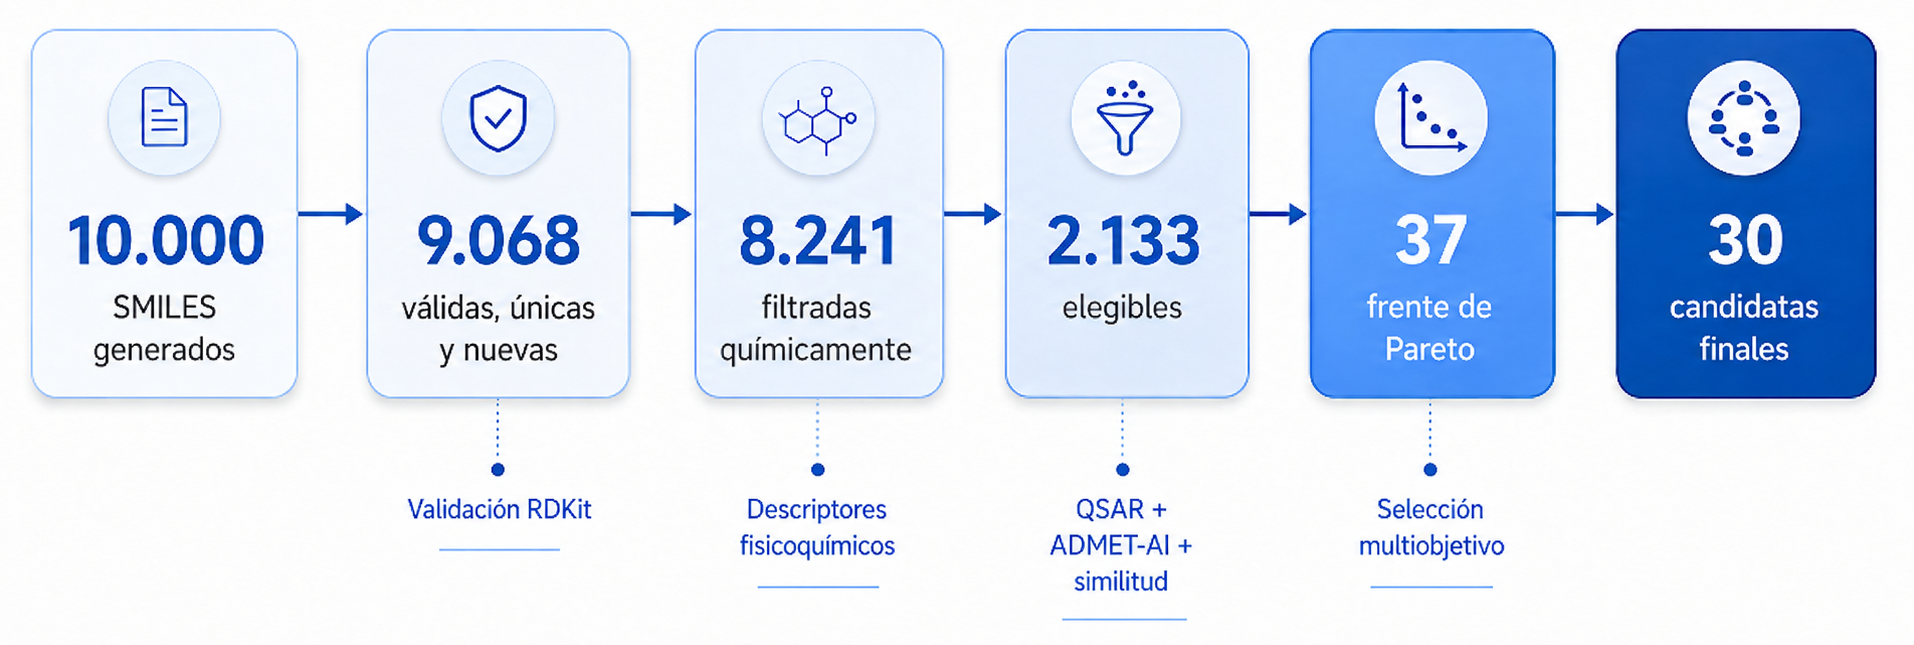
\includegraphics[width=0.95\textwidth]{resultados_figuras/fig_01_reduccion_pipeline.png}
    \caption{Reducción progresiva del conjunto molecular durante el flujo computacional.}
    \label{fig:reduccion_pipeline}
\end{figure}

La Tabla~\ref{tab:resumen_reduccion_pipeline_resultados} cuantifica esta reducción. El resultado muestra que el conjunto final de candidatas no procede directamente del modelo generativo, sino de un proceso posterior de cribado y priorización. Esta distinción es importante: el modelo generativo proporciona un espacio inicial de búsqueda, mientras que la calidad final del conjunto seleccionado depende de la evaluación multiobjetivo posterior.

\begin{table}[H]
    \centering
    \small
    \begin{tabular}{p{7.8cm} r p{3.8cm}}
        \hline
        \textbf{Etapa} & \textbf{Moléculas} & \textbf{Interpretación} \\
        \hline
        SMILES brutos generados & 10.000 & Muestra inicial del generador. \\
        SMILES válidos según RDKit & 9.082 & Estructuras químicamente interpretables. \\
        Moléculas válidas únicas & 9.079 & Duplicados canónicos eliminados. \\
        Moléculas válidas, únicas y nuevas frente al conjunto de entrenamiento & 9.068 & Entrada limpia a la evaluación. \\
        Moléculas tras filtro fisicoquímico básico & 8.241 & 90,88\% del conjunto limpio. \\
        Moléculas con evaluación completa & 8.241 & Actividad, ADMET, similitud y puntuaciones. \\
        Moléculas elegibles & 2.133 & 25,88\% del conjunto con evaluación. \\
        Soluciones no dominadas por Pareto & 37 & Frente de compromiso multiobjetivo. \\
        Conjunto final de candidatas & 30 & Candidatas priorizadas para análisis. \\
        \hline
    \end{tabular}
    \caption{Resumen cuantitativo de la reducción progresiva del conjunto molecular durante el flujo computacional.}
    \label{tab:resumen_reduccion_pipeline_resultados}
\end{table}

\section{Evaluación del modelo generativo}

El modelo generativo fue evaluado después de cada época del \textit{fine-tunning} mediante una muestra de control de 4.000 SMILES. Se analizaron tres métricas principales: validez RDKit, unicidad canónica y novedad frente al conjunto de entrenamiento. Estas métricas permiten comprobar si el modelo conserva capacidad para generar moléculas válidas, no repetitivas y no copiadas de forma directa del conjunto de datos usado durante el ajuste.

La Figura~\ref{fig:metricas_generativas_epoch} muestra la evolución de estas métricas durante las ocho épocas. La validez disminuyó de forma progresiva desde el 97,00\% en la primera época hasta valores cercanos al 88--89\% en las últimas épocas. La unicidad canónica permaneció muy alta durante todo el proceso, siempre por encima del 99\%. La novedad frente al conjunto de entrenamiento también se mantuvo elevada, aunque empezó a degradarse ligeramente a partir de la quinta época.

\begin{figure}[H]
    \centering
    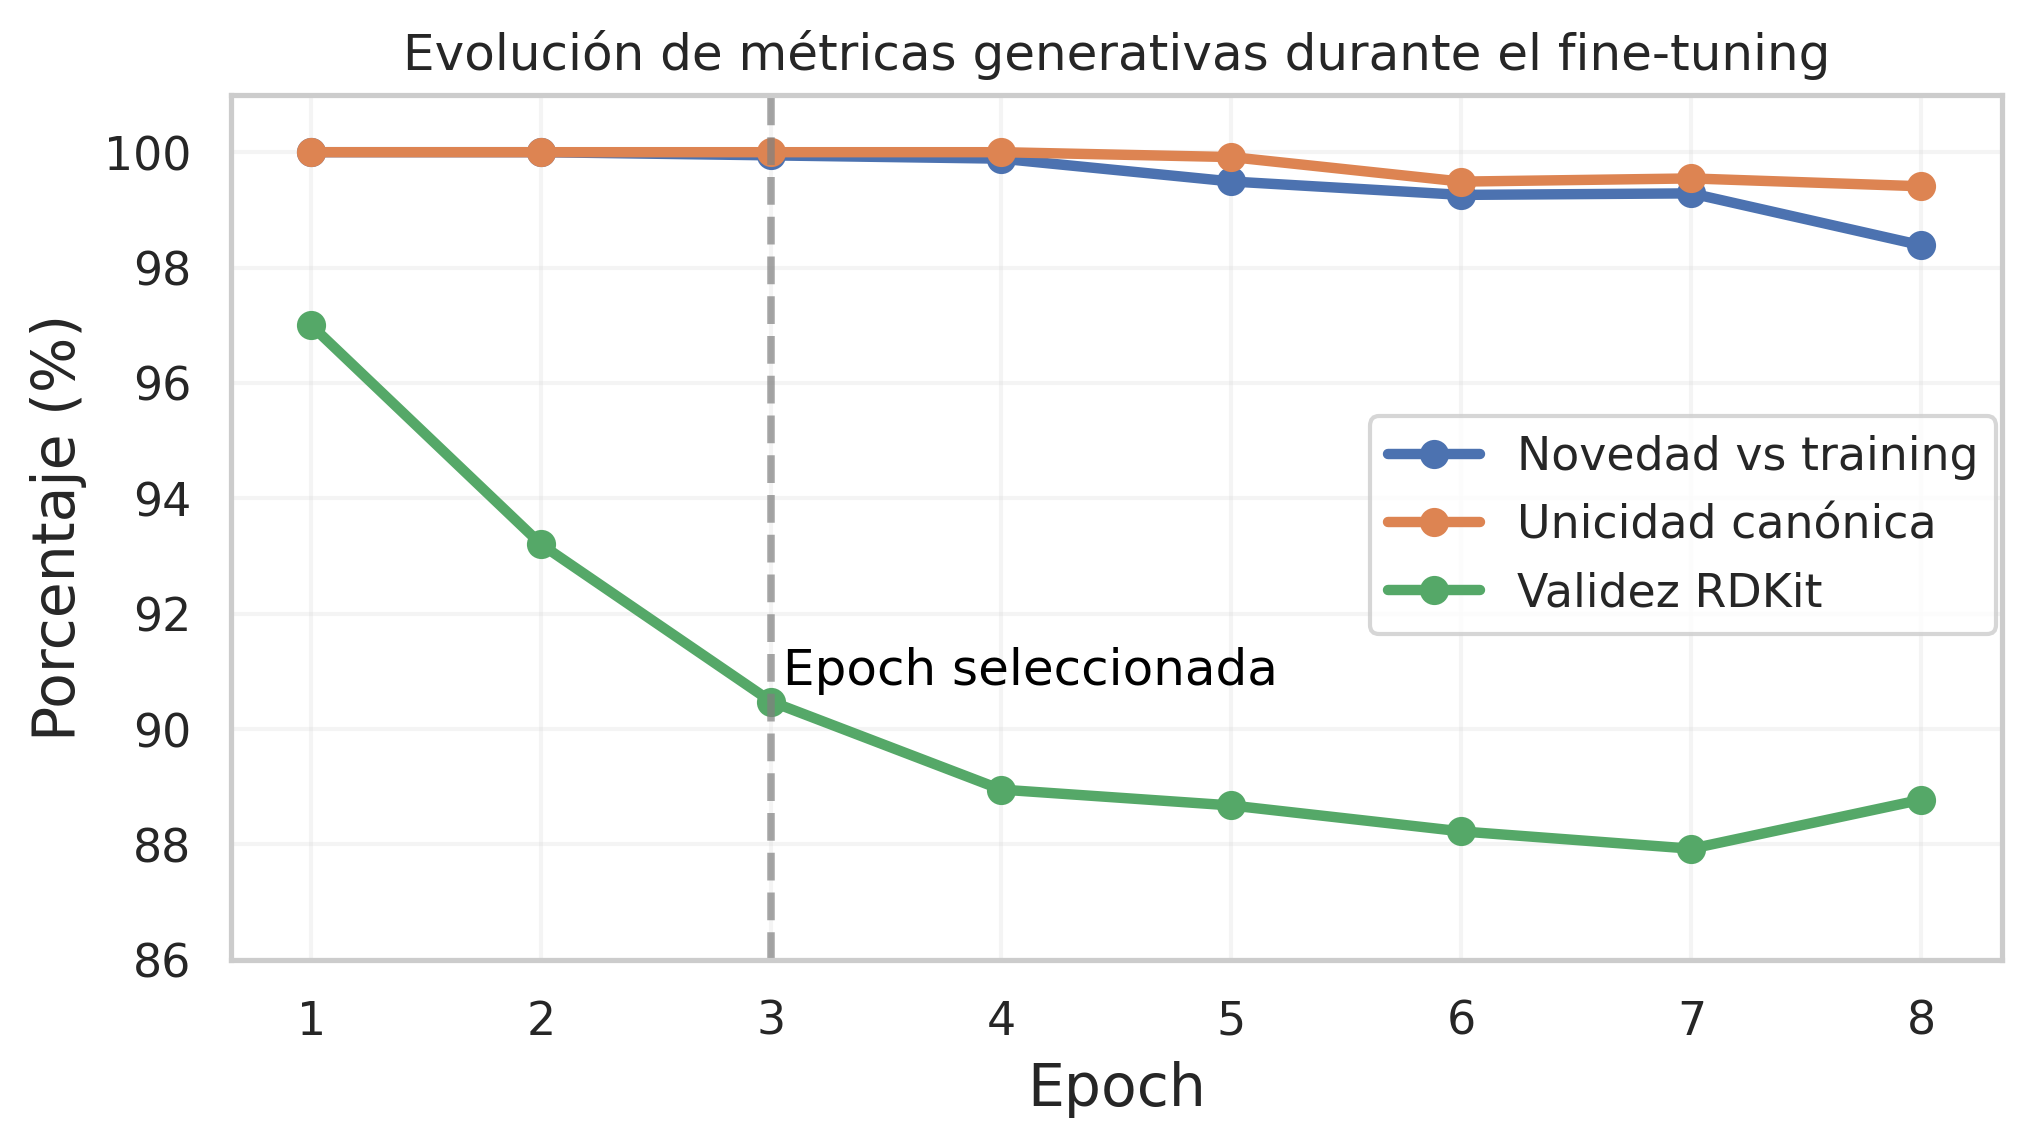
\includegraphics[width=0.72\textwidth]{resultados_figuras/fig_02_metricas_generativas_epoch.png}
    \caption{Evolución de las métricas de calidad generativa durante el ajuste fino. La línea discontinua indica la época 3, seleccionada como versión final del modelo.}
    \label{fig:metricas_generativas_epoch}
\end{figure}

La época 3 fue seleccionada como versión final del modelo porque mantenía una validez superior al 90\%, unicidad canónica del 100\% y novedad del 99,94\%. Aunque la época 1 presentaba mejores métricas brutas de validez y novedad, una única pasada por el conjunto de datos podía ser insuficiente para desplazar la distribución generativa hacia patrones químicos más compatibles con el dominio químico asociado a EGFR. Por el contrario, las épocas posteriores a la tercera no aportaron una mejora clara y comenzaron a mostrar señales de degradación progresiva en validez y novedad.

Con el modelo seleccionado se generaron 10.000 SMILES brutos. La generación final produjo 9.082 SMILES válidos, 9.079 moléculas válidas únicas y 9.068 moléculas válidas, únicas y no presentes exactamente en el conjunto de entrenamiento.

\section{Filtrado fisicoquímico y calidad molecular inicial}

Antes de aplicar modelos predictivos más costosos, las 9.068 moléculas generadas se sometieron a un filtro fisicoquímico básico basado en propiedades calculadas con RDKit. Este filtro no pretende demostrar viabilidad farmacológica, sino eliminar estructuras claramente poco plausibles para una exploración inicial de pequeñas moléculas con propiedades tipo fármaco.

Tras aplicar el filtro, se conservaron 8.241 moléculas, lo que representa el 90,88\% del conjunto limpio. Este porcentaje es relevante porque muestra que el modelo no solo generó cadenas SMILES válidas, sino una proporción alta de moléculas con rangos fisicoquímicos razonables.

\begin{figure}[H]
    \centering
    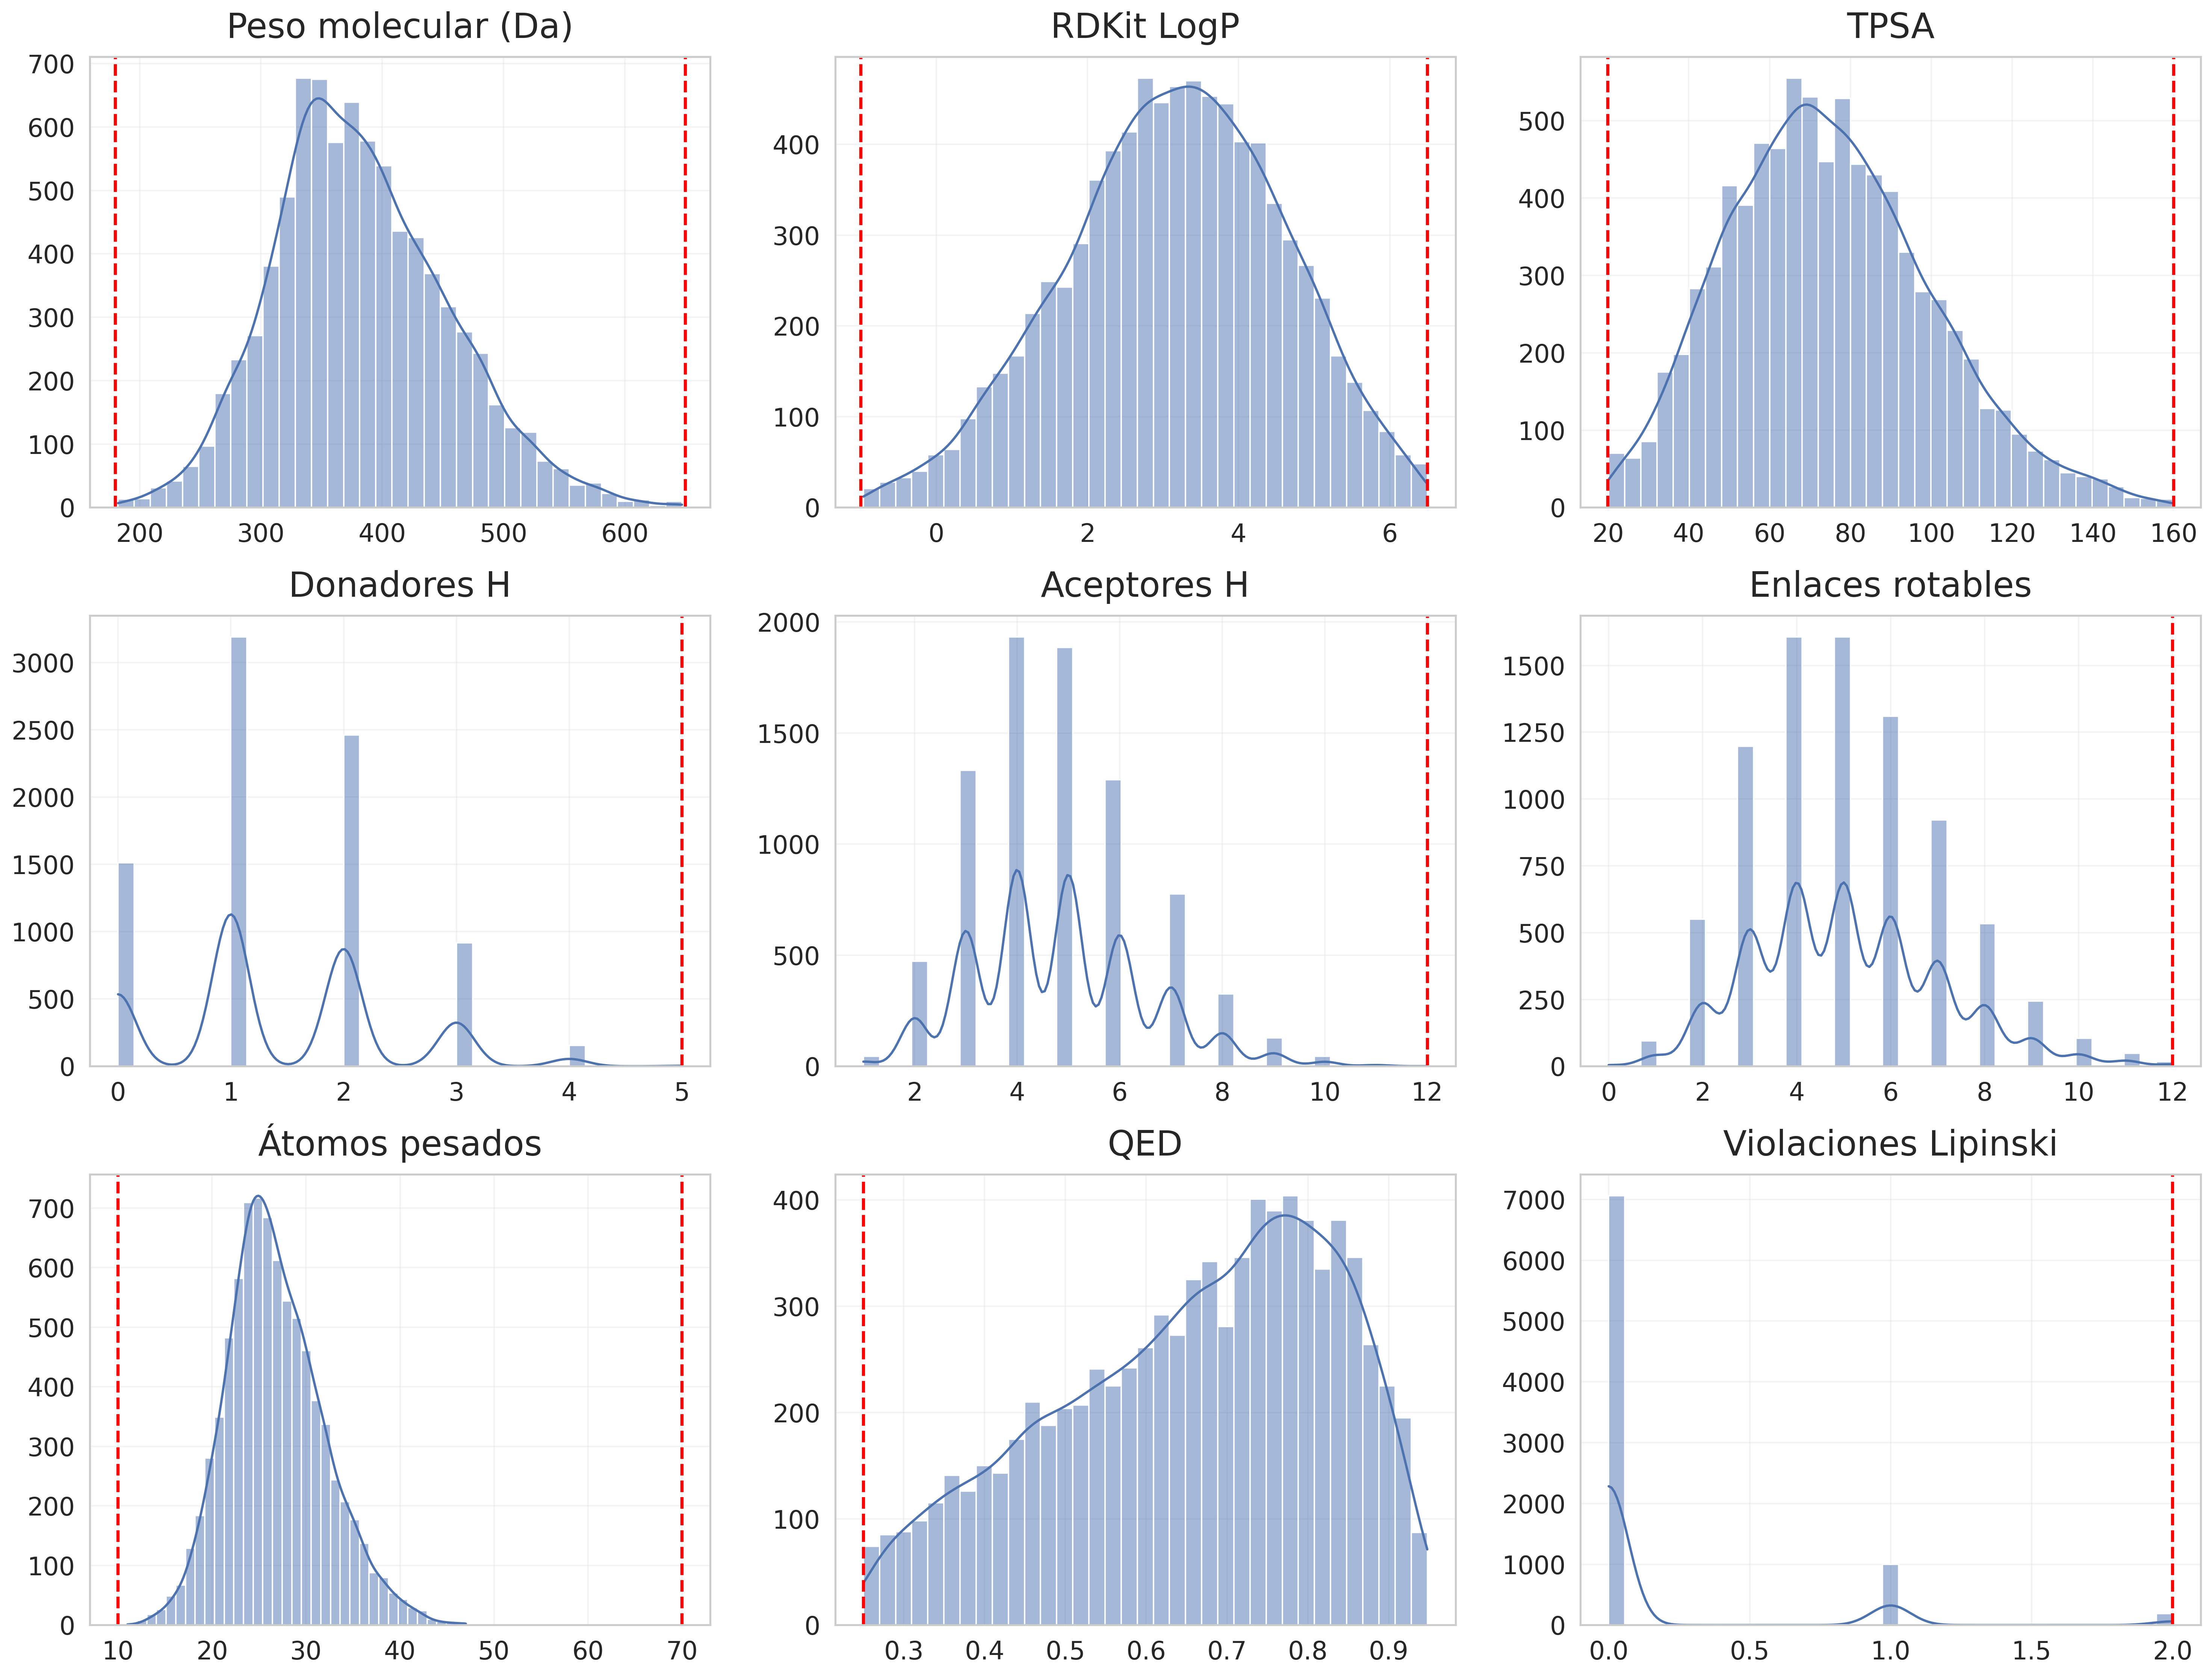
\includegraphics[width=0.95\textwidth]{resultados_figuras/fig_05_distribuciones_fisicoquimicas_filtrado.png}
    \caption{Distribución de propiedades fisicoquímicas de las moléculas que superaron el filtro básico. Las líneas verticales discontinuas indican los umbrales mínimos o máximos utilizados en cada descriptor.}
    \label{fig:distribuciones_fisicoquimicas_filtrado}
\end{figure}

La Figura~\ref{fig:distribuciones_fisicoquimicas_filtrado} muestra que las moléculas retenidas se concentran en rangos compatibles con una exploración inicial de compuestos con propiedades tipo fármaco. El peso molecular presenta una mediana de 375,45 Da y un rango intercuartílico aproximado entre 333 y 429 Da. El LogP se concentra alrededor de valores moderados, con mediana de 3,20. La TPSA se sitúa mayoritariamente en valores intermedios, con mediana de 72,95, lo que sugiere perfiles razonables de polaridad para compuestos pequeños.

La distribución de QED también es favorable en esta fase: la mediana fue 0,684 y el percentil 75 alcanzó 0,797. Además, la mayoría de moléculas no presentó violaciones de Lipinski. En conjunto, el filtrado fisicoquímico permitió conservar un conjunto amplio, pero químicamente más defendible, antes de entrar en la evaluación de actividad y ADMET.

\begin{table}[H]
    \centering
    \small
    \begin{tabular}{p{4.2cm} r r r r r}
        \hline
        \textbf{Descriptor} & \textbf{Media} & \textbf{Mediana} & \textbf{P25} & \textbf{P75} & \textbf{Rango} \\
        \hline
        Peso molecular & 382,51 & 375,45 & 333,31 & 428,87 & 182,18--647,18 \\
        RDKit LogP & 3,15 & 3,20 & 2,19 & 4,19 & -0,97--6,50 \\
        TPSA & 74,94 & 72,95 & 56,79 & 91,14 & 20,20--159,70 \\
        Donadores H & 1,4 & 1 & 1 & 2 & 0--5 \\
        Aceptores H & 4,81 & 5 & 4 & 6 & 1--12 \\
        Enlaces rotables & 5,1 & 5 & 4 & 6 & 0--12 \\
        Átomos pesados & 26,79 & 26 & 23 & 30 & 11--47 \\
        QED & 0,65 & 0,68 & 0,53 & 0,79 & 0,25--0,94 \\
        Violaciones Lipinski & 0,17 & 0 & 0 & 0 & 0--2 \\
        \hline
    \end{tabular}
    \caption{Resumen descriptivo de las moléculas que superaron el filtro fisicoquímico básico.}
    \label{tab:resumen_descriptores_filtrados_resultados}
\end{table}

\section{Modelo QSAR y actividad predicha frente a EGFR}

La actividad frente a EGFR se estimó mediante un modelo QSAR de regresión entrenado con huellas moleculares Morgan y evaluado mediante partición por scaffold de Murcko. Esta partición es más exigente que una división aleatoria, ya que reduce la probabilidad de evaluar el modelo sobre moléculas estructuralmente muy cercanas a las del entrenamiento.

El conjunto de referencia quedó dividido en 8.402 moléculas de entrenamiento, 1.065 de validación y 999 de prueba. La Tabla~\ref{tab:metricas_qsar_resultados} muestra el rendimiento obtenido.

\begin{table}[H]
    \centering
    \small
    \begin{tabular}{l c c c c}
        \hline
        \textbf{Conjunto} & \textbf{MAE} & \textbf{RMSE} & \textbf{$R^2$} & \textbf{Spearman} \\
        \hline
        Validación & 0,648 & 0,830 & 0,584 & 0,773 \\
        Prueba & 0,649 & 0,833 & 0,605 & 0,798 \\
        \hline
    \end{tabular}
    \caption{Rendimiento del modelo QSAR de regresión para la estimación de pIC$_{50}$ frente a EGFR.}
    \label{tab:metricas_qsar_resultados}
\end{table}

El modelo mostró un comportamiento razonable para una tarea de priorización temprana. La correlación de Spearman de 0,798 en prueba indica que el modelo conserva capacidad de ordenación relativa. Sin embargo, el MAE cercano a 0,65 unidades de pIC$_{50}$ impide interpretar las predicciones como valores exactos de potencia biológica. Por tanto, la pIC$_{50}$ predicha se utilizó como señal aproximada de actividad y no como evidencia directa de afinidad experimental.

Al aplicar el modelo sobre las 8.241 moléculas filtradas, la pIC$_{50}$ predicha presentó una media de 6,140 y una mediana de 6,108. En total, 5.445 moléculas fueron clasificadas como activas predichas ($pIC_{50} \geq 6$) y 162 como fuertemente activas ($pIC_{50} \geq 7$). Este resultado confirma que el generador ajustado al dominio químico asociado a EGFR produjo una cantidad relevante de moléculas con señal de actividad favorable, pero también muestra la necesidad de una selección posterior: actividad predicha por sí sola no basta para definir candidatas defendibles.

\section{Similitud estructural y control de dominio}

La novedad estructural se analizó mediante la similitud máxima de Tanimoto frente al conjunto de entrenamiento utilizado durante el \textit{fine-tunning}. Esta métrica permite detectar dos situaciones problemáticas. Por un lado, moléculas demasiado similares al conjunto de entrenamiento pueden ser análogos triviales. Por otro lado, moléculas demasiado alejadas pueden situarse fuera del dominio aproximado de aplicabilidad del modelo QSAR.

En el conjunto filtrado se detectaron dos moléculas con similitud igual o superior a 0,95 frente al conjunto de entrenamiento, consideradas casi copias estructurales. También se observó que 5.100 moléculas tenían similitud inferior a 0,30, lo que sugiere mayor incertidumbre en la extrapolación del modelo predictivo. Por ello, la etapa de elegibilidad exigió una similitud mínima de 0,30 y excluyó las casi copias con Tanimoto igual o superior a 0,95.

La relación entre similitud al conjunto de entrenamiento y actividad predicha mostró una tendencia esperable: las moléculas más próximas al dominio del entrenamiento tendieron a presentar valores medios de pIC$_{50}$ más altos. Por ejemplo, las moléculas con Tanimoto entre 0,50 y 0,70 presentaron una media de pIC$_{50}$ de 6,910, mientras que las moléculas con Tanimoto inferior a 0,25 presentaron una media de 6,007. Esta observación no demuestra mayor actividad real, pero sí indica que el modelo QSAR asigna mejores predicciones a regiones químicas más próximas a las vistas durante su entrenamiento.

\section{ADMET y definición del conjunto elegible}

Las predicciones ADMET-AI se integraron con dos niveles de lectura. En primer lugar, se definieron filtros duros para criterios considerados críticos, como alertas estructurales, toxicidad, hERG, biodisponibilidad oral y absorción intestinal. En segundo lugar, se calculó una puntuación ADMET blanda basada en percentiles frente a moléculas aprobadas de DrugBank.

La fracción media de filtros ADMET duros superados en las 8.241 moléculas con evaluación fue 0,880, con una mediana de 0,889. El valor mínimo fue 0,333 y el máximo 1,000. En cambio, el \texttt{admet\_score} blando mostró muy poca variabilidad en esta ejecución, con media 0,339 y desviación estándar 0,004. Por ese motivo, la interpretación de ADMET se apoyó principalmente en los filtros duros y, especialmente, en el criterio hERG.

Antes de aplicar Pareto se definió un conjunto de moléculas elegibles. Esta etapa fue necesaria para evitar que el frente de Pareto conservara moléculas formalmente no dominadas pero débiles desde el punto de vista farmacológico o químico. Los criterios mínimos fueron: superar el filtro fisicoquímico básico, no ser coincidencia exacta ni casi copia del conjunto de entrenamiento, presentar similitud mínima al conjunto de entrenamiento de 0,30, tener pIC$_{50}$ predicha igual o superior a 6,0 y superar al menos el 75\% de los filtros ADMET duros.

La aplicación conjunta de estos criterios redujo el conjunto de 8.241 moléculas con evaluación a 2.133 moléculas elegibles, equivalente al 25,88\%. Esta fue una de las etapas más selectivas del flujo computacional, ya que combinó actividad estimada, control de similitud y señales ADMET antes de la optimización multiobjetivo.

\section{Selección mediante dominancia de Pareto}

Una vez definido el conjunto elegible, se aplicó selección multiobjetivo mediante dominancia de Pareto. Como resultado, las 2.133 moléculas elegibles se redujeron a 37 soluciones no dominadas. Posteriormente, estas soluciones se ordenaron por \texttt{reward\_score}, utilizado únicamente como criterio auxiliar de priorización, y se aplicó un control de diversidad por scaffold de Murcko. El conjunto final de candidatas quedó formado por 30 moléculas.

Dado que la selección se realizó sobre seis objetivos, el frente de Pareto no puede representarse fielmente en dos dimensiones sin perder información. Por ello, la Figura~\ref{fig:pareto_parallel} utiliza coordenadas paralelas. Cada línea representa una molécula y cada eje vertical corresponde a uno de los objetivos normalizados.

\begin{figure}[H]
    \centering
    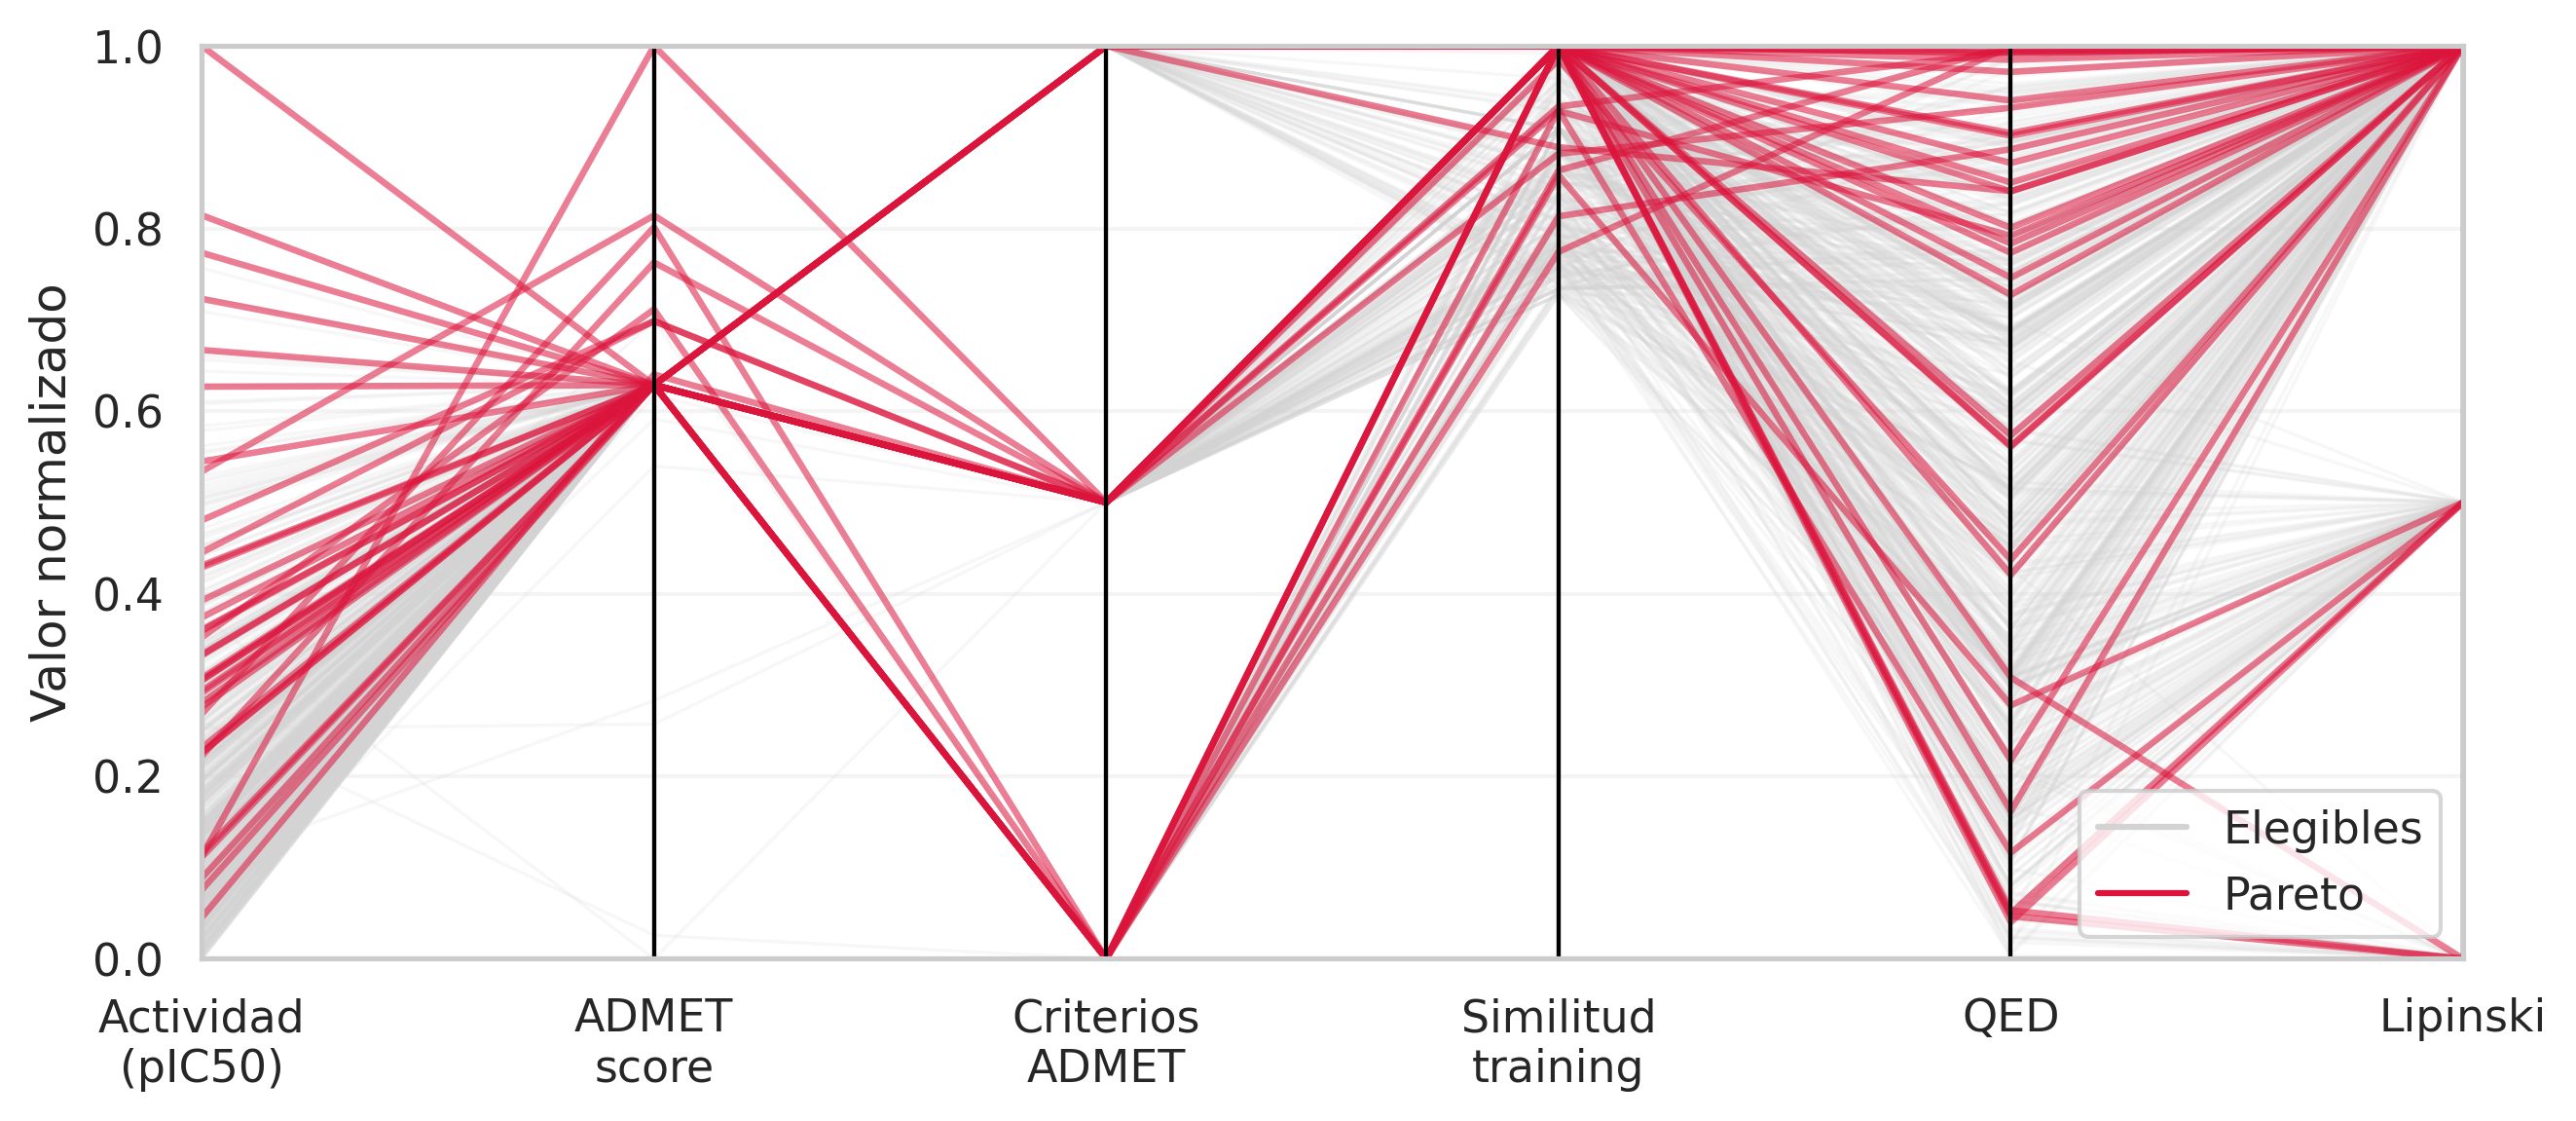
\includegraphics[width=\textwidth]{resultados_figuras/fig_pareto_parallel_eligible_vs_pareto.png}
    \caption{Representación mediante coordenadas paralelas de los objetivos utilizados en la selección multiobjetivo. Las moléculas elegibles se muestran en gris y las soluciones no dominadas por Pareto se destacan en rojo. Todos los valores se normalizaron entre 0 y 1.}
    \label{fig:pareto_parallel}
\end{figure}

La Figura~\ref{fig:pareto_parallel} muestra que las soluciones no dominadas no responden a un único patrón. Algunas moléculas destacan por actividad predicha, otras por QED, otras por cumplimiento ADMET y otras por mejor posición respecto a la ventana de similitud al conjunto de entrenamiento. Este resultado justifica el uso de Pareto: seleccionar únicamente las moléculas con mayor pIC$_{50}$ habría producido una lectura incompleta y más arriesgada.

\section{Distribución global del conjunto final de candidatas}

El conjunto final de 30 candidatas concentra moléculas con actividad predicha favorable, buena calidad molecular global y diversidad estructural. La Figura~\ref{fig:shortlist_distribuciones_globales} resume las principales variables utilizadas para interpretar el conjunto final.

\begin{figure}[H]
    \centering
    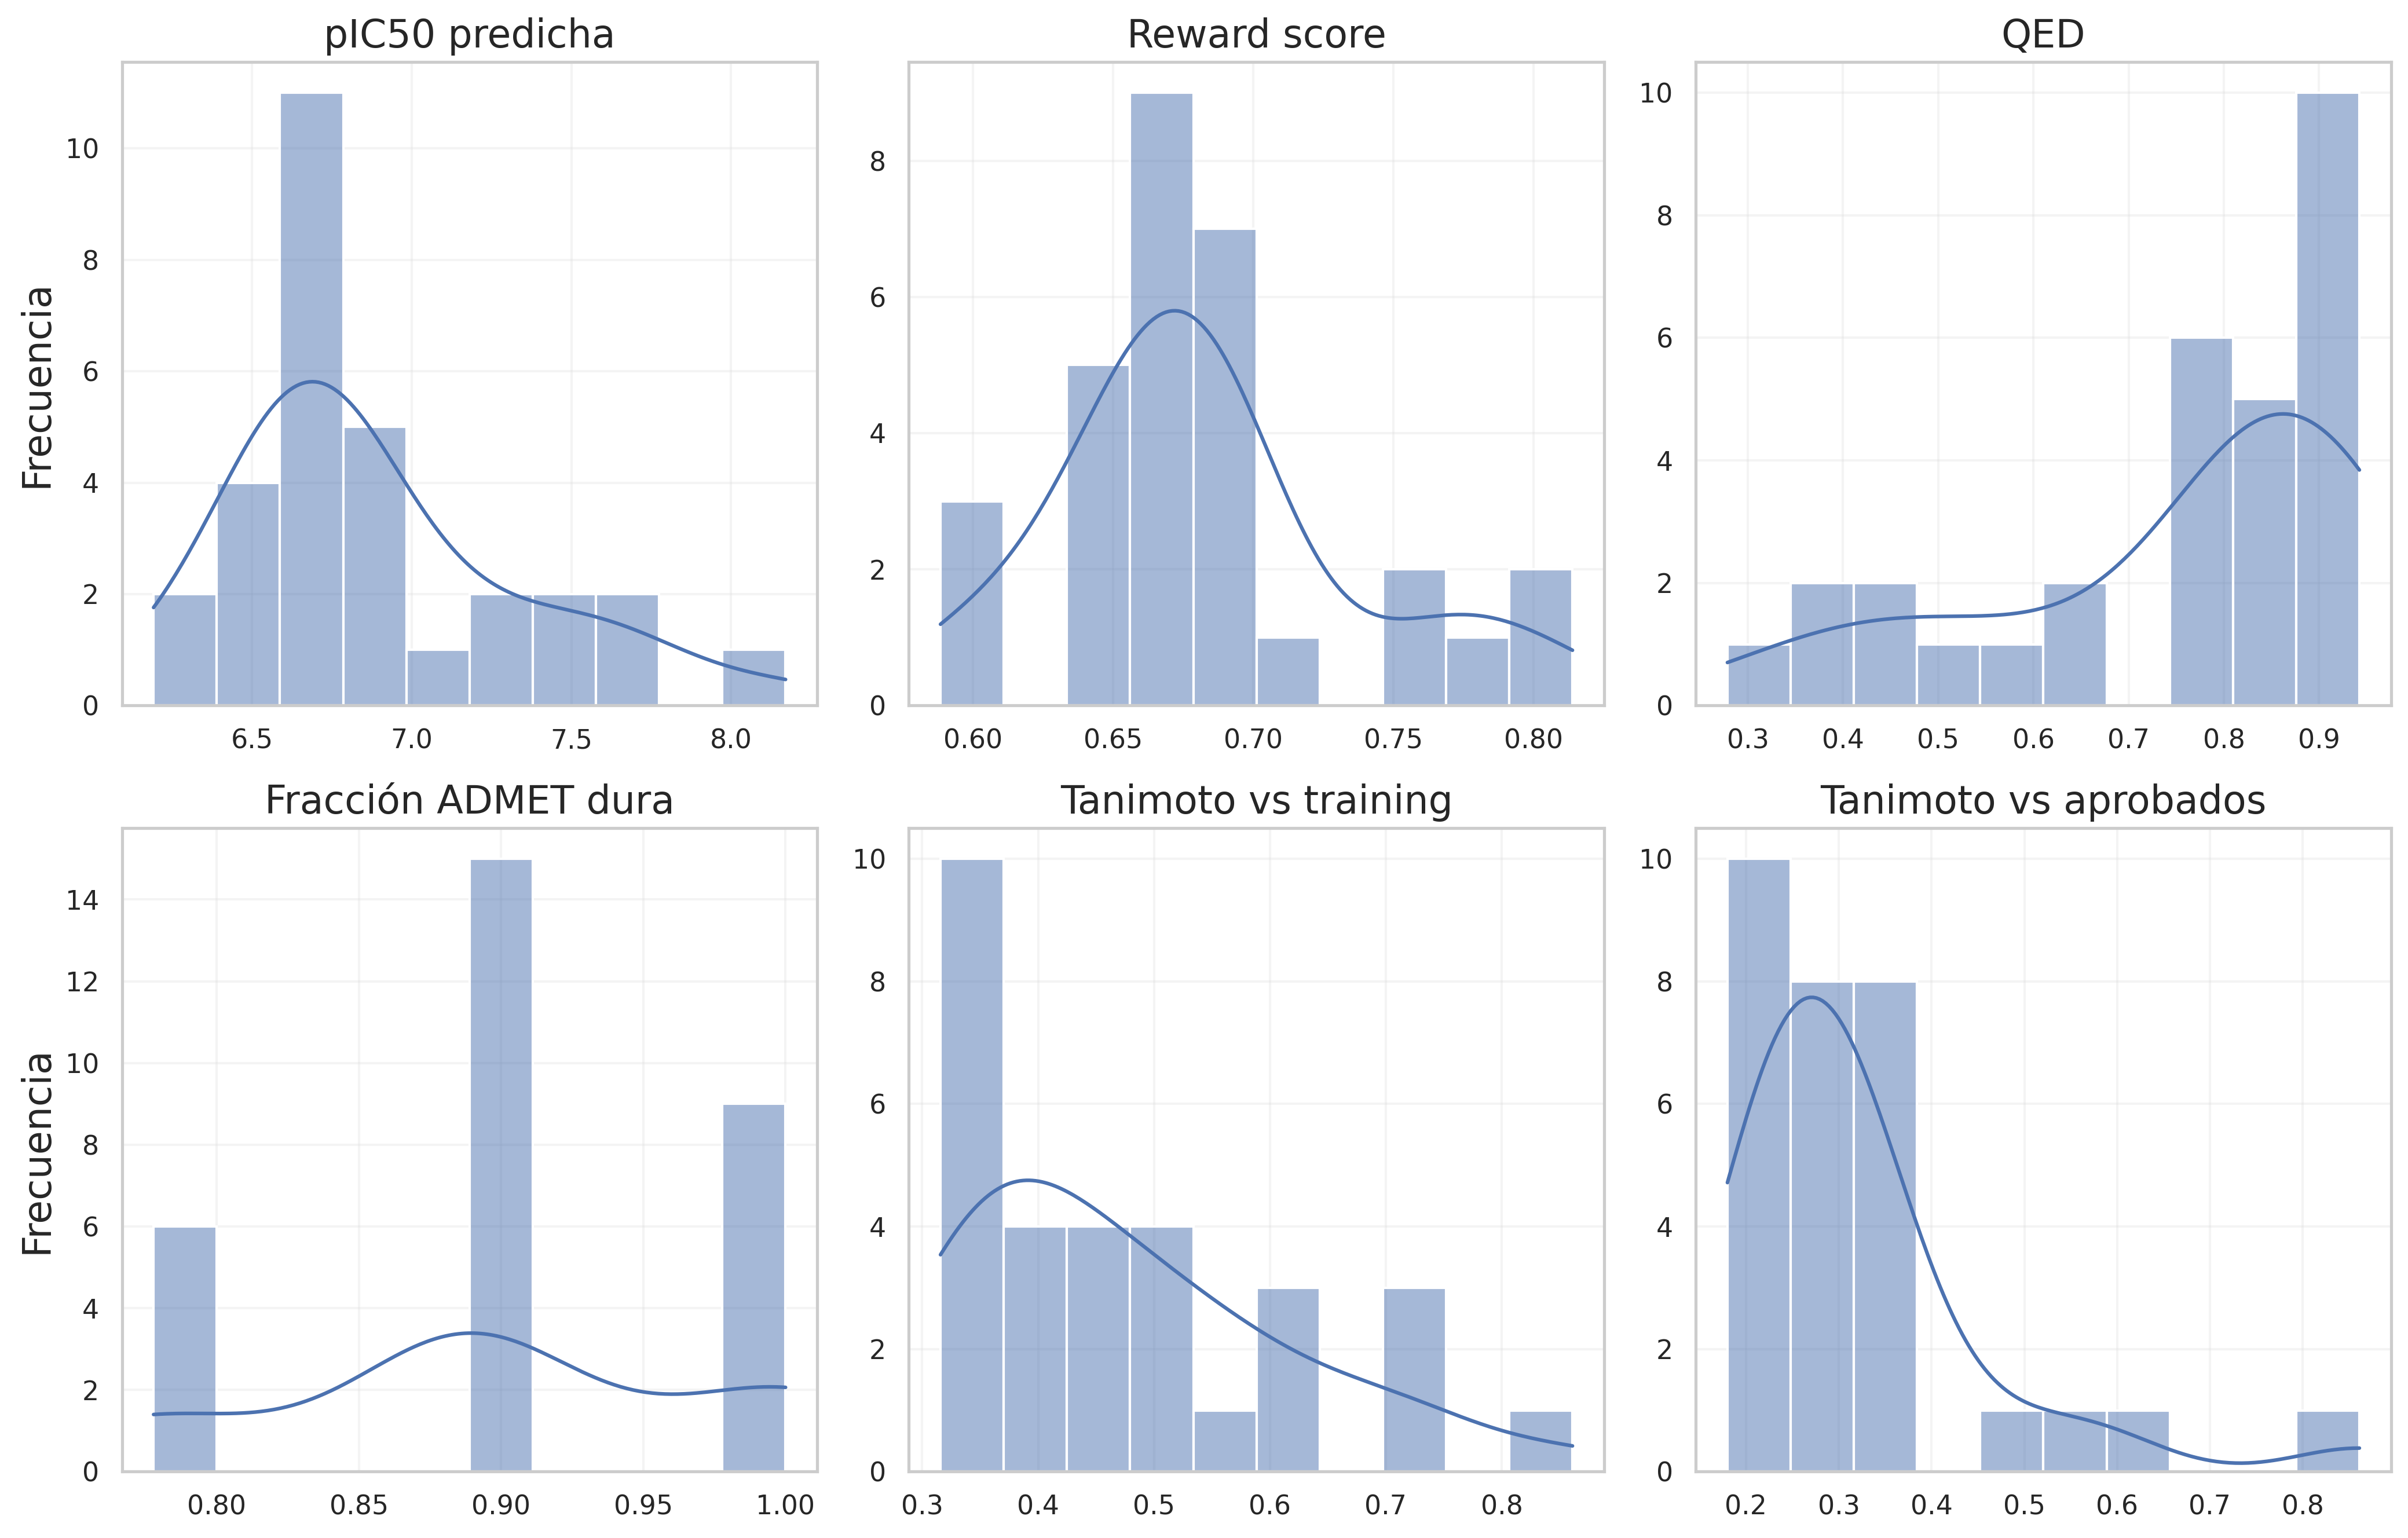
\includegraphics[width=\textwidth]{resultados_figuras/fig_02_distribuciones_shortlist.png}
    \caption{Distribución de métricas clave en el conjunto final de 30 candidatas: pIC$_{50}$ predicha, \texttt{reward\_score}, QED, fracción de criterios ADMET superados, similitud máxima frente al conjunto de entrenamiento y similitud máxima frente a inhibidores EGFR aprobados o de referencia.}
    \label{fig:shortlist_distribuciones_globales}
\end{figure}

La Tabla~\ref{tab:resumen_shortlist_resultados} resume estadísticamente el conjunto final de candidatas. La pIC$_{50}$ predicha media fue 6,891, con una mediana de 6,751 y un valor máximo de 8,171. El QED medio fue 0,749, con una mediana de 0,821, lo que indica que el conjunto final está enriquecido en moléculas con propiedades tipo fármaco favorables. La fracción media de criterios ADMET duros superados fue 0,900, aunque este valor debe interpretarse junto con el análisis individual de criterios, ya que \textbf{hERG} aparece como el principal criterio problemático.

\begin{table}[H]
    \centering
    \small
    \begin{tabular}{p{4.5cm} r r r r r}
        \hline
        \textbf{Variable} & \textbf{Media} & \textbf{Mediana} & \textbf{P25} & \textbf{P75} & \textbf{Rango} \\
        \hline
        pIC$_{50}$ predicha & 6,89 & 6,75 & 6,62 & 7,11 & 6,19--8,17 \\
        \texttt{reward\_score} & 0,68 & 0,68 & 0,65 & 0,70 & 0,59--0,81 \\
        QED & 0,75 & 0,82 & 0,64 & 0,89 & 0,28--0,94 \\
        Violaciones Lipinski & 0,13 & 0 & 0 & 0 & 0--2 \\
        Fracción ADMET dura & 0,90 & 0,89 & 0,89 & 1 & 0,78--1 \\
        \hline
    \end{tabular}
    \caption{Resumen descriptivo de las principales métricas del conjunto final de candidatas.}
    \label{tab:resumen_shortlist_resultados}
\end{table}

La Figura~\ref{fig:actividad_qed_reward} complementa esta lectura mostrando la relación entre actividad predicha y QED. El tamaño de los puntos es proporcional a la puntuación global \texttt{reward\_score}. Esta visualización es útil porque permite detectar que una mayor pIC$_{50}$ predicha no implica necesariamente mejor calidad molecular. En particular, algunas candidatas de alta actividad presentan QED más bajo, lo que refuerza la necesidad de no interpretar la actividad como único criterio de selección.

\begin{figure}[H]
    \centering
    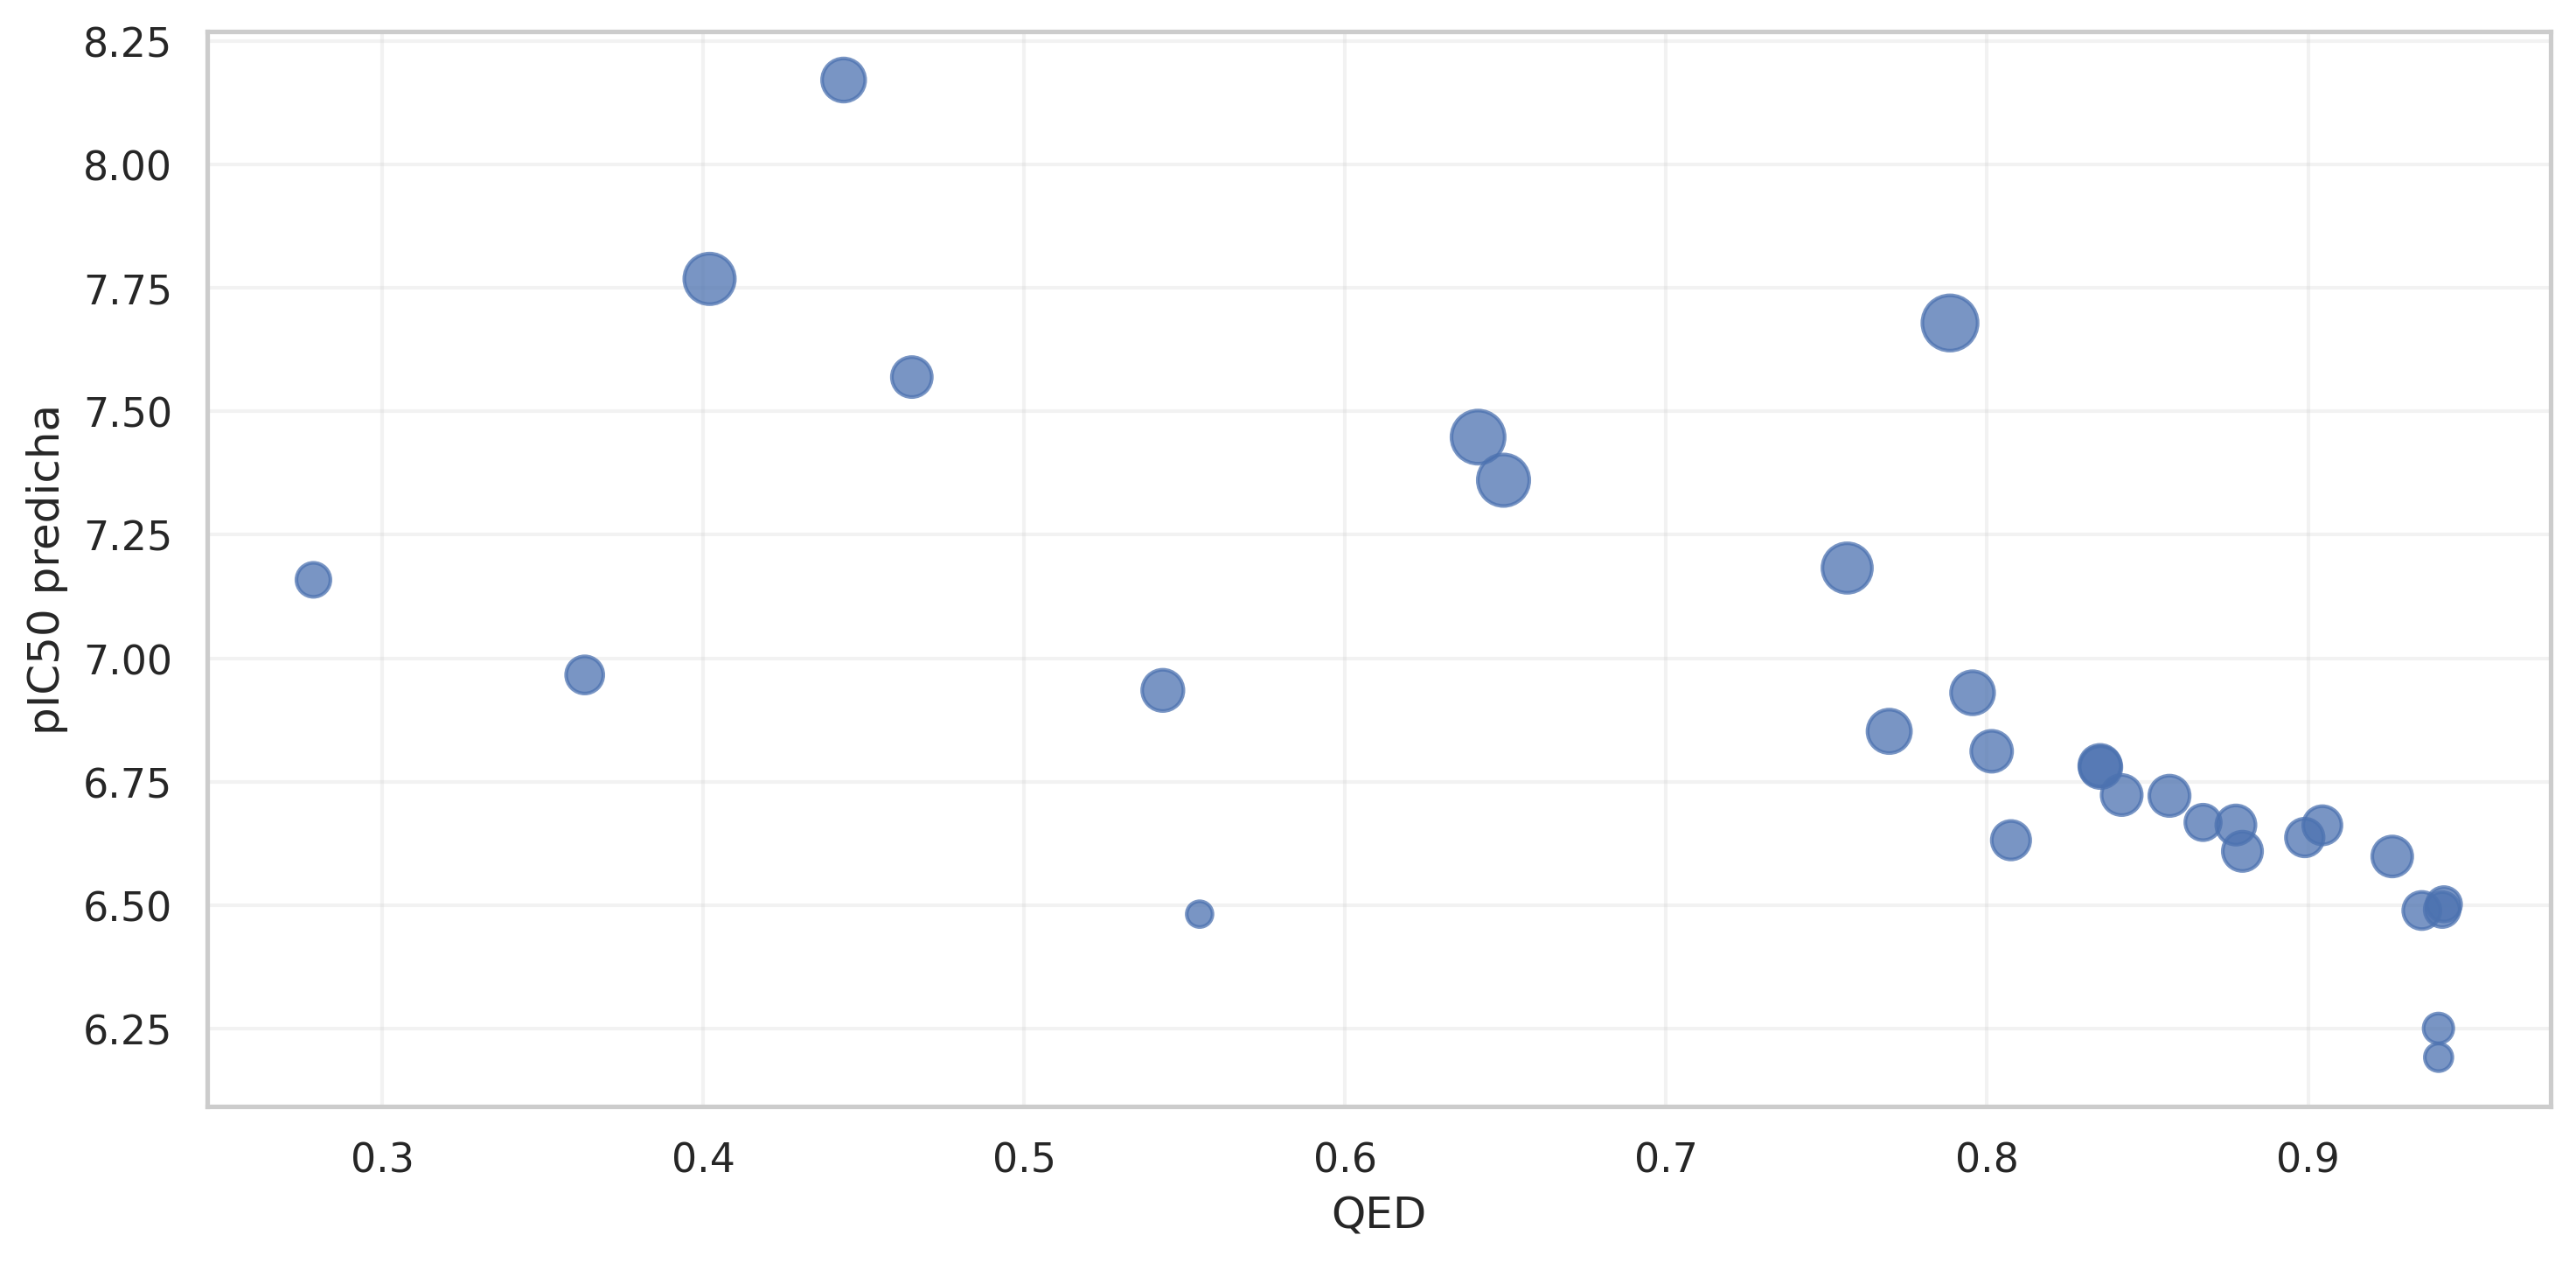
\includegraphics[width=0.85\textwidth]{resultados_figuras/fig_actividad_vs_qed_reward.png}
    \caption{Relación entre actividad predicha y calidad molecular tipo fármaco en el conjunto final de candidatas. El tamaño de los puntos es proporcional a la puntuación global \texttt{reward\_score}.}
    \label{fig:actividad_qed_reward}
\end{figure}

La Figura~\ref{fig:top_reward_moleculas} muestra la representación molecular de las candidatas con mayor puntuación global \texttt{reward\_score}. Esta figura no debe interpretarse como una validación estructural ni como evidencia de unión a EGFR, sino como apoyo visual para comprobar que las moléculas mejor priorizadas no son representaciones abstractas, sino estructuras químicas concretas que pueden inspeccionarse individualmente.

\begin{figure}[H]
    \centering
    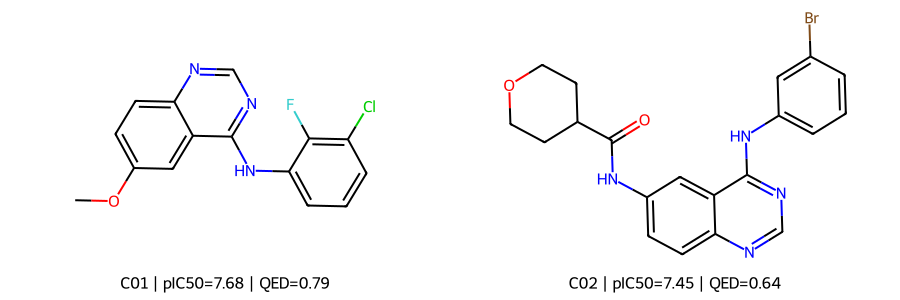
\includegraphics[width=0.85\textwidth]{resultados_figuras/fig_top10_reward_moleculas.png}
    \caption{Representación molecular de las candidatas con mayor puntuación global \texttt{reward\_score}.}
    \label{fig:top_reward_moleculas}
\end{figure}

\section{Actividad y perfil ADMET de las candidatas}

Una vez definido el conjunto final de candidatas, se analizó el cumplimiento individual de los criterios ADMET duros. La Figura~\ref{fig:shortlist_admet_heatmap} muestra qué criterios superó cada candidata. Las filas representan moléculas y las columnas corresponden a criterios ADMET relevantes.

\begin{figure}[H]
    \centering
    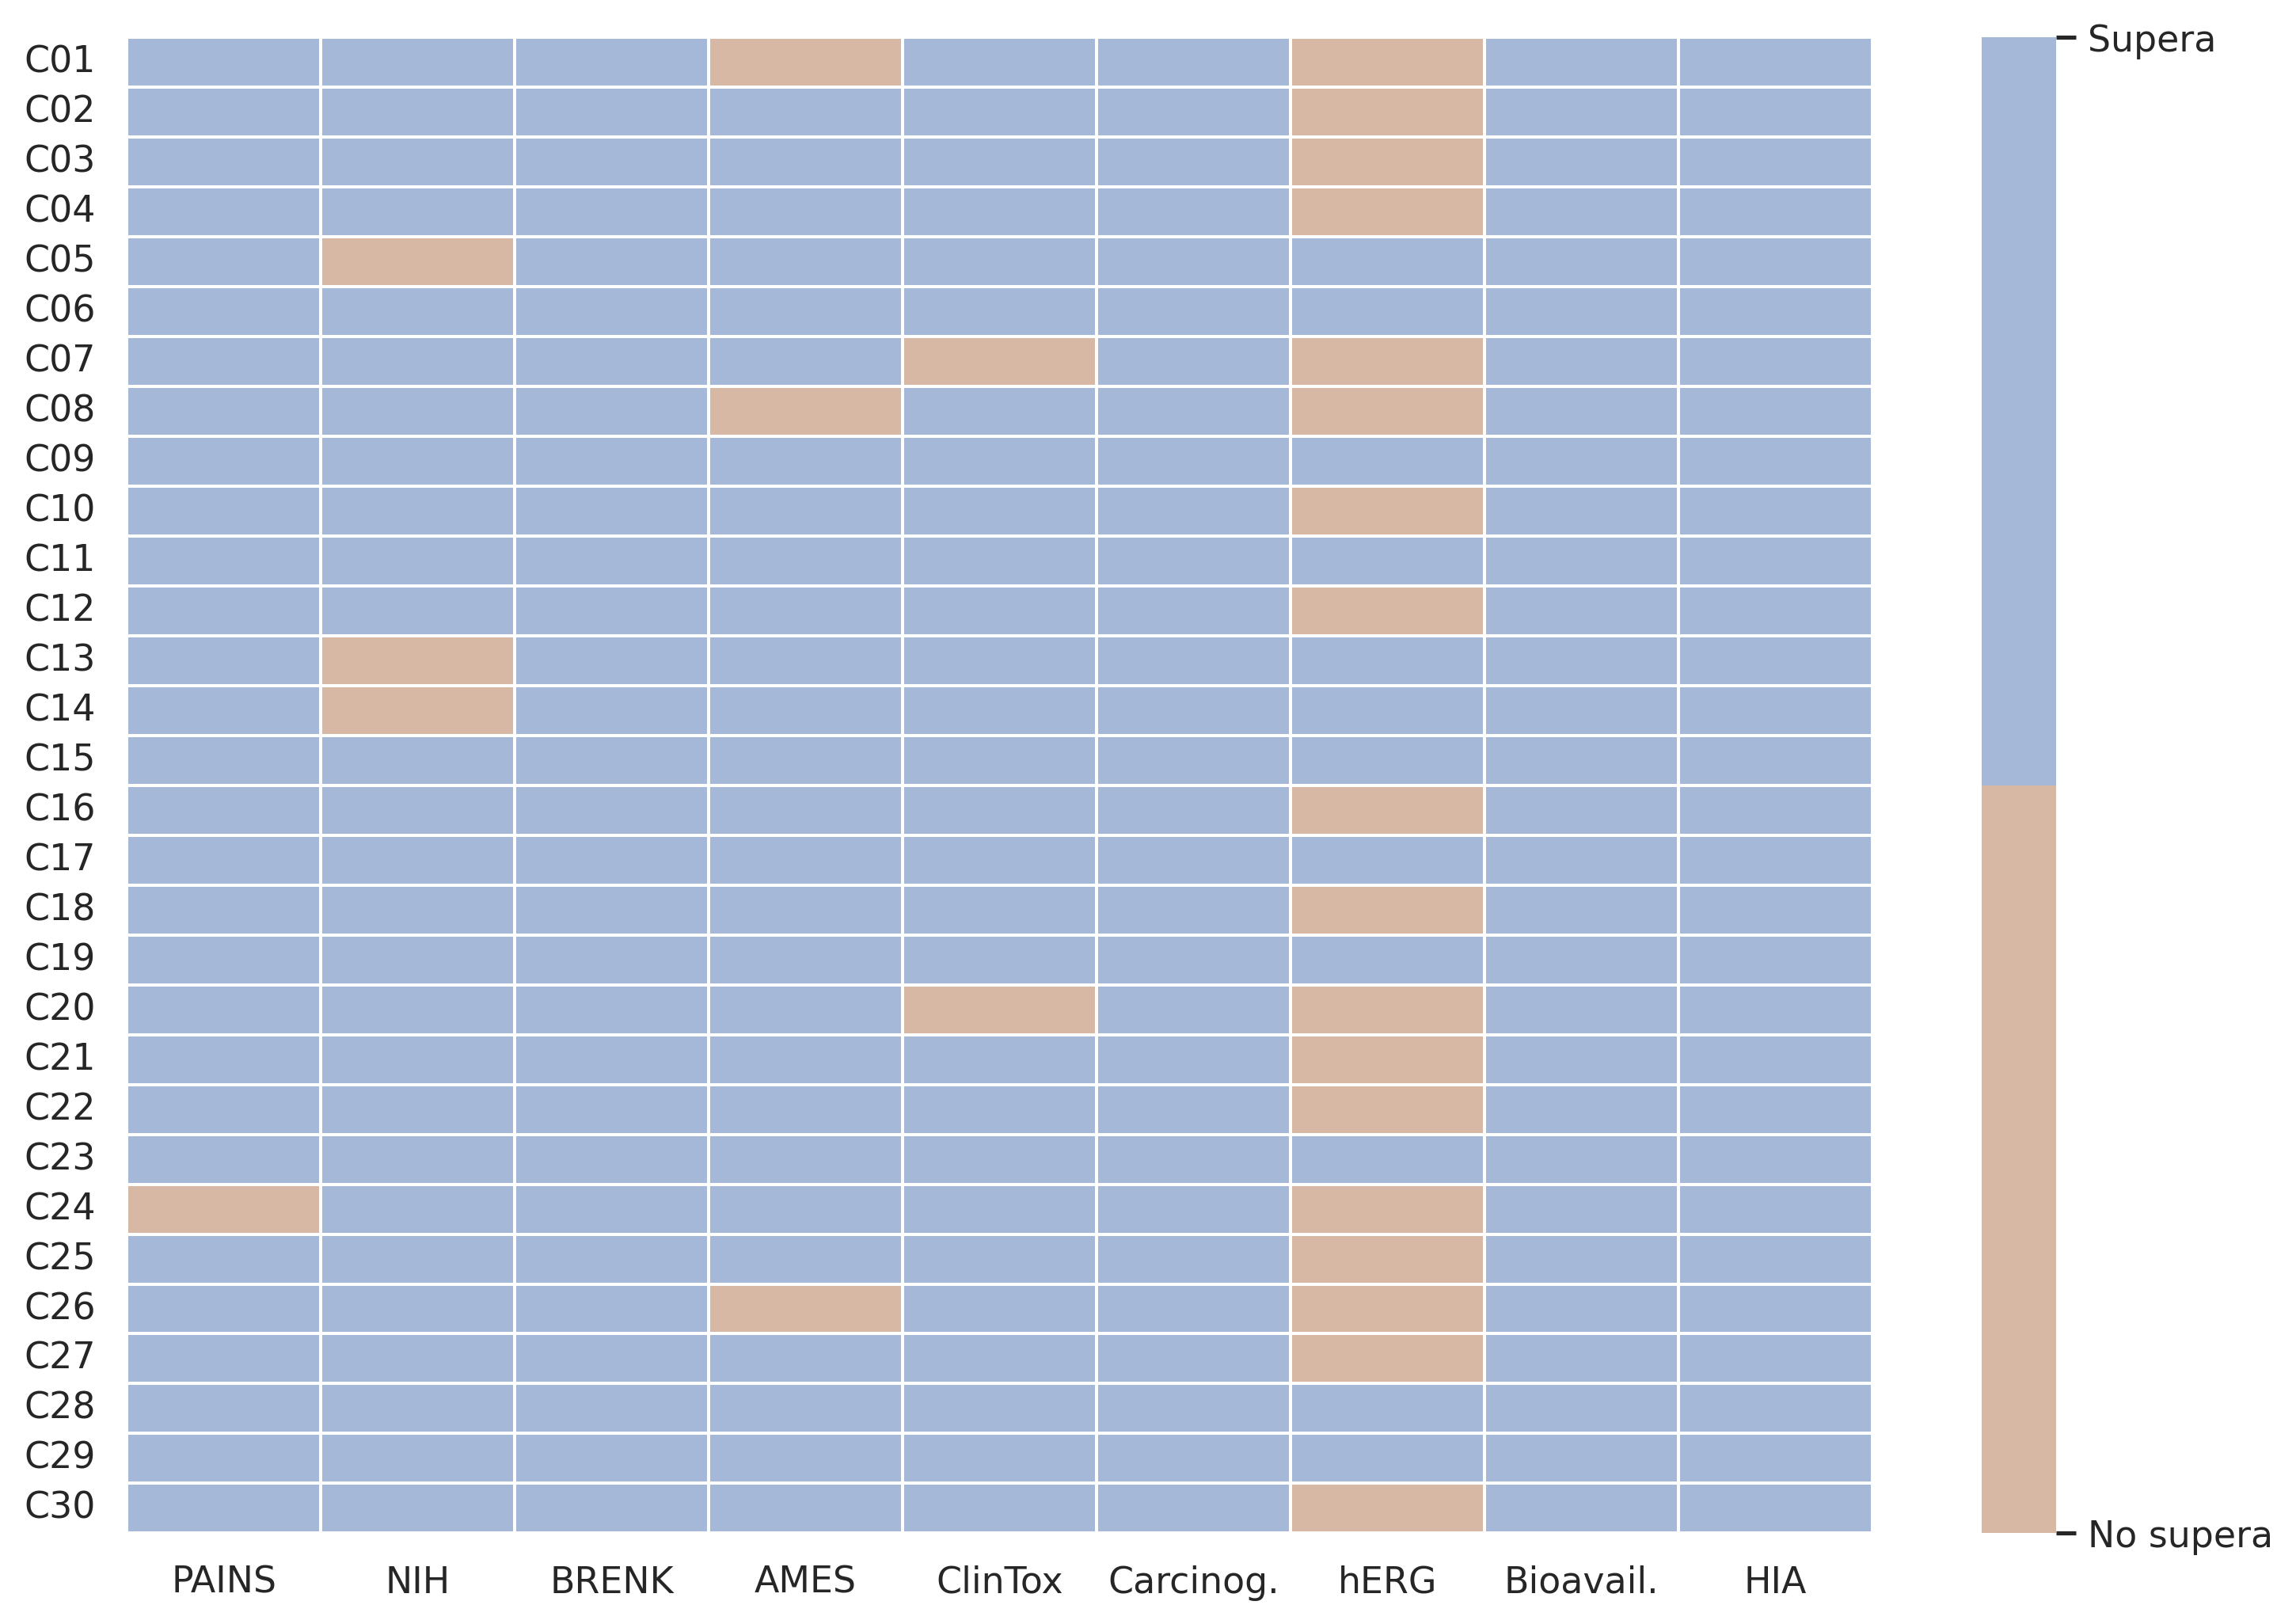
\includegraphics[width=0.88\textwidth]{resultados_figuras/fig_shortlist_admet_heatmap.png}
    \caption{Mapa de cumplimiento de criterios ADMET predichos en las moléculas candidatas finales. Las filas representan candidatas y las columnas corresponden a criterios ADMET relevantes.}
    \label{fig:shortlist_admet_heatmap}
\end{figure}

La Tabla~\ref{tab:admet_endpoint_shortlist_resultados} resume el cumplimiento por criterio. La mayoría de candidatas supera los criterios de BRENK, carcinogenicidad, biodisponibilidad oral e HIA. También se observa un cumplimiento alto en PAINS, ClinTox, NIH y AMES. Sin embargo, hERG es claramente el criterio más problemático: solo 12 de las 30 candidatas lo superan, mientras que 18 presentan una señal desfavorable.

\begin{table}[H]
    \centering
    \small
    \begin{tabular}{l c c c}
        \hline
        \textbf{Criterio} & \textbf{Superan} & \textbf{No superan} & \textbf{Porcentaje superado} \\
        \hline
        hERG & 12 & 18 & 40,00\% \\
        NIH & 27 & 3 & 90,00\% \\
        AMES & 27 & 3 & 90,00\% \\
        ClinTox & 28 & 2 & 93,33\% \\
        PAINS & 29 & 1 & 96,67\% \\
        BRENK & 30 & 0 & 100,00\% \\
        Carcinogenicidad & 30 & 0 & 100,00\% \\
        Biodisponibilidad & 30 & 0 & 100,00\% \\
        HIA & 30 & 0 & 100,00\% \\
        \hline
    \end{tabular}
    \caption{Cumplimiento de criterios ADMET duros en el conjunto final de candidatas.}
    \label{tab:admet_endpoint_shortlist_resultados}
\end{table}

Este resultado es uno de los puntos críticos del análisis. El conjunto final de candidatas presenta buenos valores globales de actividad y calidad molecular, pero no puede describirse como un conjunto ADMET completamente limpio. El fallo de hERG en 18 candidatas introduce un riesgo computacional relevante, asociado a posible cardiotoxicidad. Por ello, hERG debe tratarse como una alerta independiente y no quedar escondido dentro de la fracción global de criterios superados.

La Figura~\ref{fig:shortlist_actividad_admet} muestra la relación entre pIC$_{50}$ predicha y fracción de criterios ADMET duros superados. El color indica si la molécula supera o no el criterio hERG.

\begin{figure}[H]
    \centering
    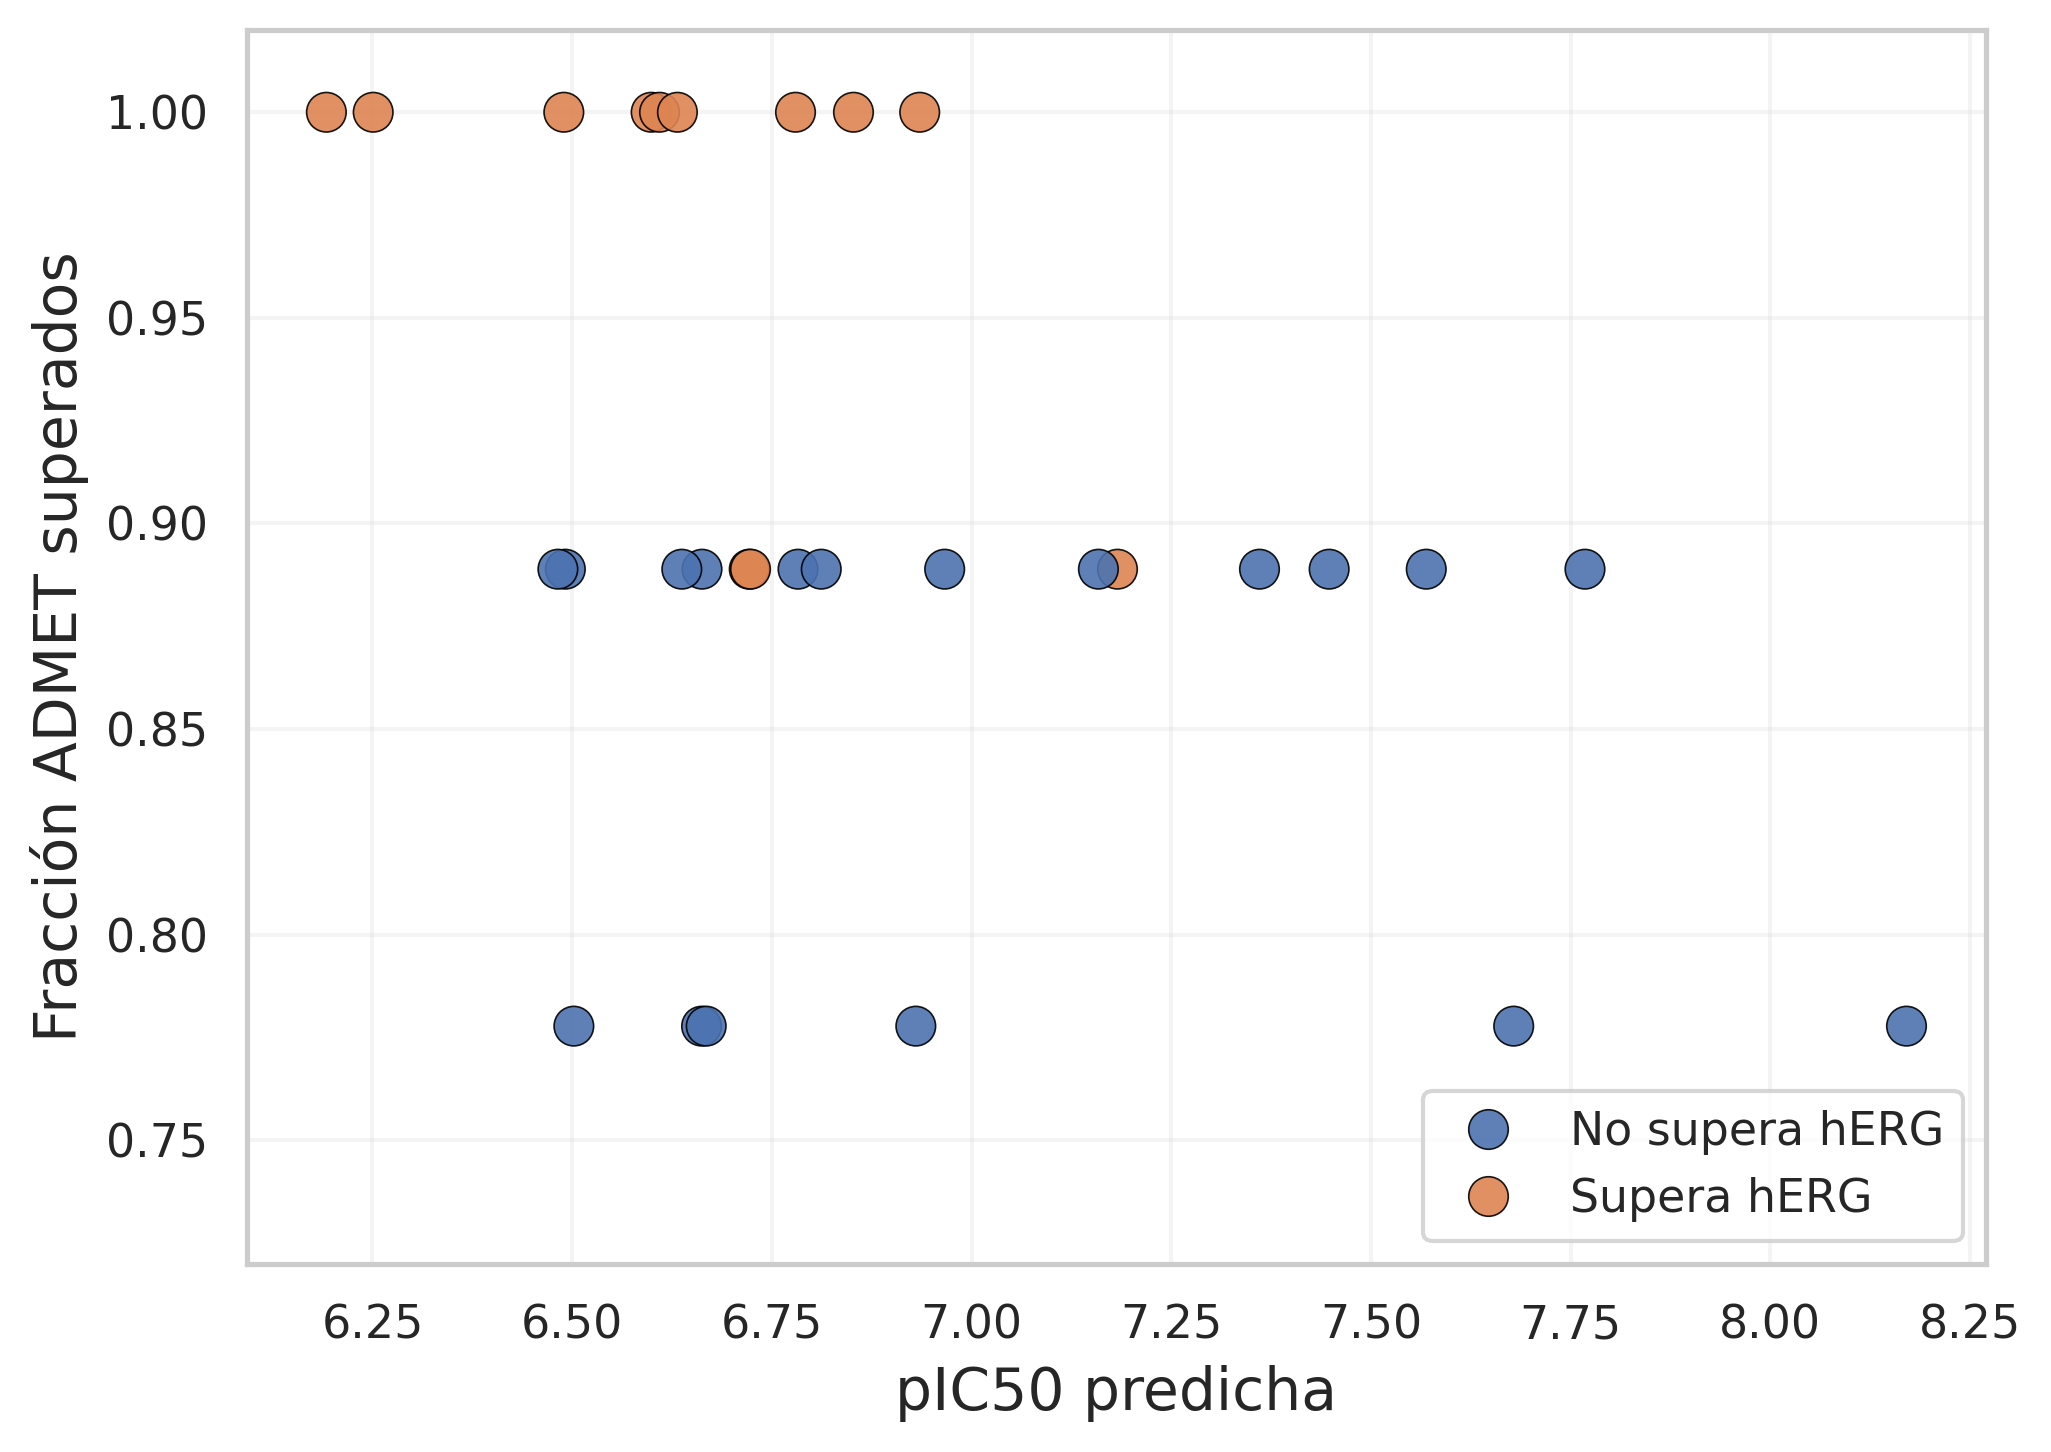
\includegraphics[width=0.68\textwidth]{resultados_figuras/fig_shortlist_pIC50_vs_admet.png}
    \caption{Relación entre la actividad predicha frente a EGFR y la fracción de criterios ADMET superados en las moléculas candidatas finales. Cada punto representa una candidata; el color indica si supera o no el criterio hERG.}
    \label{fig:shortlist_actividad_admet}
\end{figure}

La figura muestra que todas las candidatas conservan una señal de actividad favorable, con pIC$_{50}$ predicha superior a 6. No obstante, también evidencia que mayor actividad predicha no equivale necesariamente a mejor perfil ADMET. Algunas moléculas con alta pIC$_{50}$ estimada no superan hERG o presentan menor fracción de criterios ADMET superados. Por tanto, las candidatas más defendibles no son simplemente las más activas, sino aquellas que combinan actividad razonable, QED favorable, ausencia de violaciones fisicoquímicas graves y menor riesgo ADMET computacional.

\section{Novedad estructural}

La novedad estructural se evaluó desde dos perspectivas. Primero, se calculó la similitud máxima de Tanimoto frente al conjunto de entrenamiento utilizado en el ajuste fino, para valorar si las candidatas eran copias o análogos demasiado cercanos. Segundo, se compararon las candidatas con un conjunto de inhibidores EGFR aprobados, con el objetivo de detectar posibles análogos obvios de fármacos conocidos.

La comparación frente a inhibidores EGFR aprobados mostró que 26 de las 30 candidatas se clasificaron como de alta novedad frente a aprobados, 3 como relacionadas medicinalmente y 1 como análogo cercano de aprobado. Este resultado aporta interés exploratorio al conjunto final de candidatas, aunque también aumenta la incertidumbre externa: una molécula más novedosa puede ser más original, pero no necesariamente más plausible desde el punto de vista experimental.

La Figura~\ref{fig:actividad_training_tanimoto} representa la actividad predicha frente a la similitud máxima al conjunto de entrenamiento. El color corresponde a la puntuación global \texttt{reward\_score}. Muestra cómo se distribuyen las candidatas finales entre actividad estimada y cercanía al dominio de entrenamiento.

\begin{figure}[H]
    \centering
    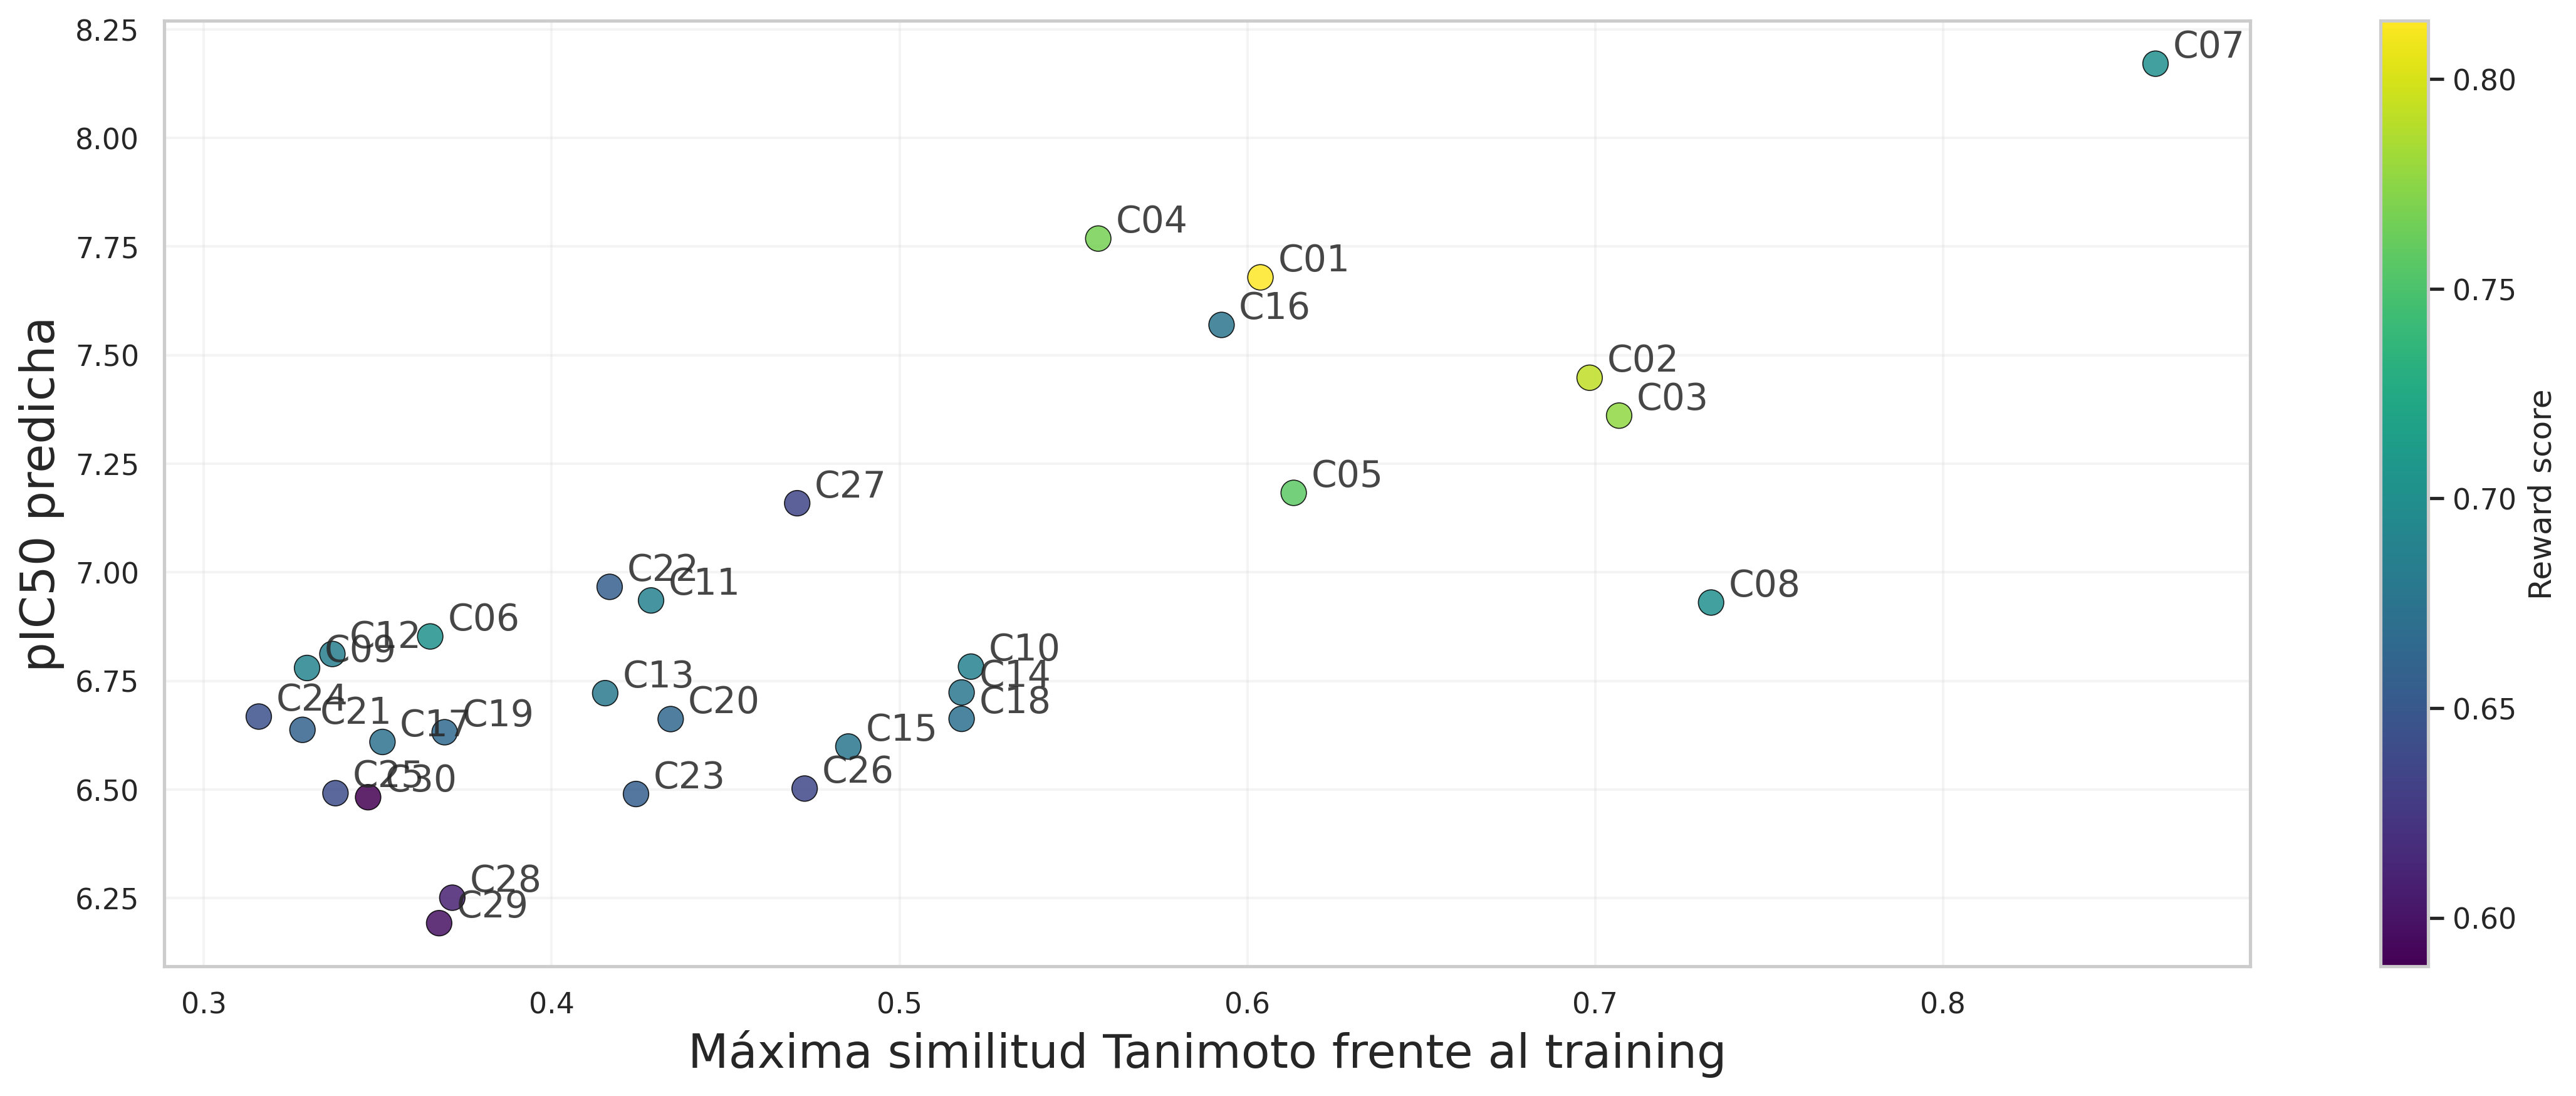
\includegraphics[width=0.9\textwidth]{resultados_figuras/fig_shortlist_tanimoto_training_vs_approved.png}
    \caption{Relación entre la pIC$_{50}$ predicha y la máxima similitud de Tanimoto frente al conjunto de entrenamiento en el conjunto final de candidatas. El color representa la puntuación global \texttt{reward\_score}.}
    \label{fig:actividad_training_tanimoto}
\end{figure}

La mayoría de candidatas se sitúa en valores de similitud moderados frente al conjunto de entrenamiento. Esto es deseable porque evita dos extremos: por un lado, moléculas casi copiadas del conjunto de entrenamiento; por otro, moléculas tan alejadas que el modelo QSAR podría estar extrapolando con baja fiabilidad. La candidata C07 constituye un caso especial: presenta la mayor pIC$_{50}$ predicha, pero también una similitud elevada tanto frente al entrenamiento como frente a dacomitinib, lo que reduce su novedad efectiva y obliga a tratarla como una hipótesis de mayor riesgo.

La Figura~\ref{fig:c07_comparacion_tanimoto} muestra precisamente la comparación estructural de C07 con dacomitinib, su referencia EGFR más cercana por Tanimoto. La comparación visual ayuda a interpretar por qué C07 no debe venderse como molécula altamente novedosa, sino como una estructura próxima a una región química conocida.

\begin{figure}[H]
    \centering
    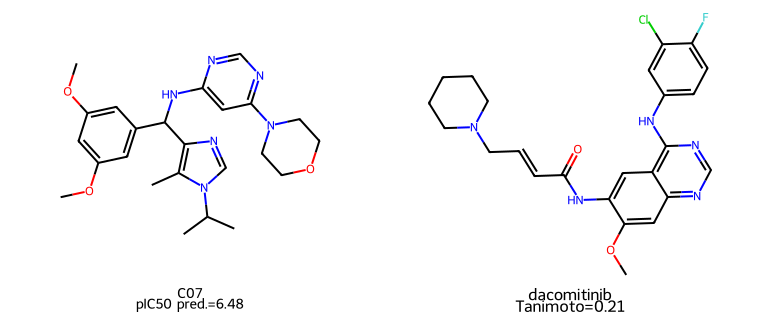
\includegraphics[width=0.75\textwidth]{resultados_figuras/fig_c07_comparacion_tanimoto.png}
    \caption{Comparación estructural de la candidata C07 con dacomitinib, inhibidor EGFR aprobado más cercano según Tanimoto.}
    \label{fig:c07_comparacion_tanimoto}
\end{figure}

\section{Diversidad química por scaffolds de Murcko}

Además de actividad y ADMET, se evaluó la diversidad estructural del conjunto final de candidatas mediante scaffolds de Murcko. Este análisis responde a una pregunta clave: si las 30 candidatas pertenecieran a una misma familia estructural, el flujo computacional habría colapsado hacia una región química estrecha. En cambio, una mayor diversidad de scaffolds indica que la selección final conserva alternativas químicas reales.

El conjunto final de candidatas contiene 29 scaffolds de Murcko distintos para 30 moléculas, lo que implica un ratio scaffold/molécula de 0,97. Este resultado indica que la selección no se concentró en una única familia química. El control de diversidad aplicado tras Pareto permitió conservar una cartera amplia de núcleos estructurales, algo especialmente útil en una etapa temprana de descubrimiento, donde conviene preservar alternativas para análisis posteriores.

\section{Perfiles interpretativos de candidatas}

El conjunto final de candidatas no debe interpretarse como una ordenación lineal. En un problema multiobjetivo, una molécula puede ser interesante por equilibrio global, otra por actividad, otra por perfil ADMET, otra por novedad y otra por calidad tipo fármaco. Por ello, se seleccionaron perfiles representativos mediante reglas explícitas, evitando escoger candidatas de forma arbitraria.

La Tabla~\ref{tab:perfiles_candidatas_resultados} resume cinco perfiles interpretativos: C05 como candidata más equilibrada con hERG favorable, C07 como molécula con mayor actividad predicha, C06 como mejor perfil ADMET general, C23 como mayor novedad frente a aprobados y C26 como mejor calidad molecular tipo fármaco según QED.

\begin{table}[H]
    \centering
    \small
    \renewcommand{\arraystretch}{1.35}
    \begin{tabular}{p{1cm} p{5cm} p{10cm}}
        \hline
        \textbf{ID} & \textbf{Perfil} & \textbf{Lectura principal} \\
        \hline
        C05 & Más equilibrada con hERG favorable & Buen compromiso global, aunque presenta fallo NIH. \\

        C07 & Mayor actividad predicha & Hipótesis potente, pero con QED bajo, alerta hERG y alta similitud con dacomitinib. \\

        C06 & Mejor perfil ADMET general & Perfil prudente: cumple todos los filtros ADMET duros y mantiene actividad favorable. \\

        C23 & Mayor novedad & Molécula exploratoria, muy alejada de inhibidores EGFR aprobados, con mayor incertidumbre externa. \\

        C26 & Mejor calidad tipo fármaco & QED muy alto, pero penalizada por hERG y AMES. \\
        \hline
    \end{tabular}
    \caption{Candidatas representativas de distintos perfiles dentro del conjunto final de candidatas. ADMET corresponde a la fracción de filtros ADMET duros superados.}
    \label{tab:perfiles_candidatas_resultados}
\end{table}

La Figura~\ref{fig:perfiles_moleculares} muestra la representación molecular de estos perfiles. La visualización confirma que no se trata simplemente de variantes triviales de una misma molécula, sino de estructuras con diferencias apreciables en núcleos y sustituyentes.

\begin{figure}[H]
    \centering
    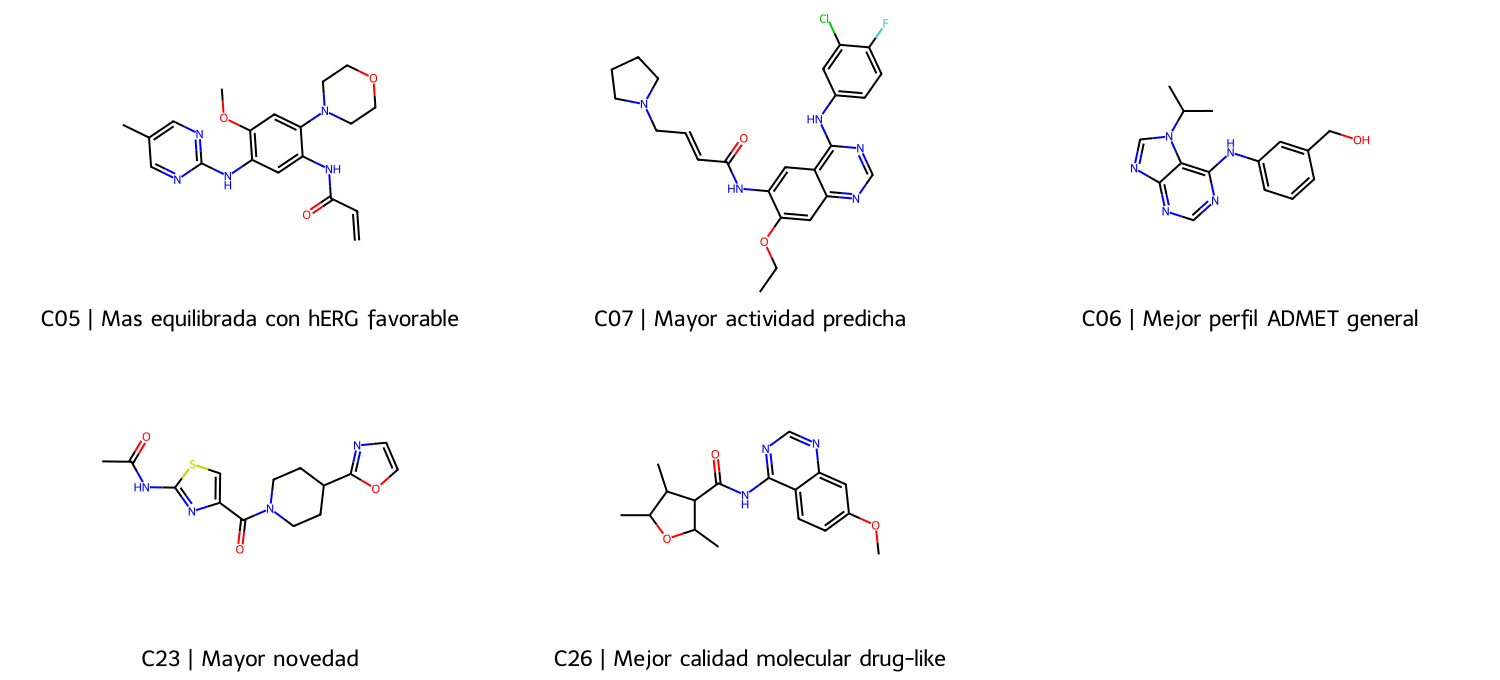
\includegraphics[width=1\textwidth]{resultados_figuras/fig_perfiles_moleculares.png}
    \caption{Representación molecular de las candidatas seleccionadas como perfiles interpretativos: C05 como perfil equilibrado, C07 como alta actividad predicha, C06 como mejor perfil ADMET general, C23 como mayor novedad y C26 como mejor calidad tipo fármaco.}
    \label{fig:perfiles_moleculares}
\end{figure}

La candidata C05 representa el mejor compromiso global entre actividad, puntuación global \texttt{reward\_score}, QED y hERG favorable, aunque no está completamente libre de alertas, ya que presenta fallo en NIH. C07 es la molécula con mayor actividad predicha, pero concentra varias señales de riesgo: no supera hERG, presenta QED bajo, tiene una violación de Lipinski y muestra alta similitud con dacomitinib. Por tanto, C07 debe describirse como una hipótesis de alta actividad pero alto riesgo, no como la mejor candidata global.

C06 es la candidata más limpia desde el punto de vista ADMET general, ya que supera todos los filtros duros considerados, incluido hERG. Aunque su actividad predicha no es la máxima, su perfil equilibrado la convierte en una de las moléculas más defendibles para priorización conservadora. C23 destaca por novedad frente a inhibidores EGFR aprobados y por QED alto, pero su actividad es más moderada y su distancia estructural aumenta la incertidumbre del modelo. Finalmente, C26 presenta el QED más alto, pero falla hERG y AMES, por lo que no puede considerarse una candidata segura pese a su buena calidad tipo fármaco.

\section{Riesgos detectados en el conjunto final de candidatas}

Para evitar una interpretación excesivamente optimista, se construyeron indicadores de riesgo sobre el conjunto final de candidatas. Se consideraron señales como fallos ADMET generales, fallo hERG, alta similitud frente al conjunto de entrenamiento, QED bajo y exceso de violaciones de Lipinski.

La Tabla~\ref{tab:riesgos_shortlist_resultados} resume los resultados. De las 30 candidatas, 21 presentan al menos una señal de riesgo y 9 no presentan señales críticas bajo los criterios definidos. El riesgo más frecuente es hERG, presente en 18 candidatas. Además, 9 candidatas presentan algún fallo ADMET general excluyendo hERG.

\begin{table}[H]
    \centering
    \small
    \begin{tabular}{p{8cm} c}
        \hline
        \textbf{Indicador} & \textbf{Número de candidatas} \\
        \hline
        Candidatas con al menos una señal de riesgo & 21 \\
        Candidatas sin señales de riesgo bajo los criterios definidos & 9 \\
        Candidatas que no superan hERG & 18 \\
        Candidatas con fallos ADMET generales excluyendo hERG & 9 \\
        \hline
    \end{tabular}
    \caption{Resumen de señales de riesgo detectadas en el conjunto final de candidatas.}
    \label{tab:riesgos_shortlist_resultados}
\end{table}

\chapter{Conclusiones y trabajos futuros}

\section{Conclusiones}

Este Trabajo Final de Máster ha permitido comprobar que una \textit{pipeline} computacional modular puede transformar una muestra amplia de moléculas generadas en una cartera reducida de hipótesis moleculares priorizadas frente a EGFR. La principal aportación del trabajo no es proponer una molécula concreta como inhibidor validado, sino construir un flujo reproducible capaz de generar, filtrar, ordenar e interpretar moléculas bajo criterios explícitos de actividad predicha, calidad molecular, perfil ADMET, novedad estructural y diversidad química.

La primera conclusión relevante es que la generación molecular, por sí sola, no basta para obtener candidatas defendibles. El modelo generativo produjo 10.000 SMILES brutos, de los cuales se obtuvieron 9.068 moléculas válidas, únicas y no presentes exactamente en el conjunto de entrenamiento. Sin embargo, tras aplicar el filtro fisicoquímico, los criterios de elegibilidad, la selección por dominancia de Pareto y el control final de diversidad, el conjunto quedó reducido a 30 candidatas. Esta reducción progresiva muestra que el valor del enfoque no reside únicamente en generar muchas moléculas, sino en disponer de una estrategia posterior capaz de descartar, priorizar y justificar qué moléculas merecen análisis adicional.

El modelo QSAR resultó útil como herramienta de priorización relativa, pero no debe interpretarse como una medida experimental de actividad. En el conjunto de prueba obtuvo una correlación de Spearman de 0,798, lo que indica una capacidad razonable para ordenar moléculas según actividad predicha. No obstante, el MAE de 0,649 unidades de pIC$_{50}$ impide tratar diferencias pequeñas entre candidatas como diferencias reales de potencia biológica. Por tanto, la pIC$_{50}$ predicha se ha utilizado correctamente como señal \textit{proxy}, combinándola con ADMET, QED, reglas de Lipinski y similitud estructural.

El conjunto final de 30 candidatas presenta señales computacionales favorables, pero heterogéneas. La selección conserva diversidad estructural, con 29 scaffolds de Murcko distintos para 30 moléculas, lo que indica que el proceso no colapsó hacia una única familia química. Este resultado es importante en una etapa temprana de descubrimiento, ya que permite mantener alternativas con perfiles distintos en lugar de seleccionar únicamente análogos muy próximos entre sí.

La lectura por perfiles resulta más honesta que declarar una única molécula ganadora. C05 representa el mejor compromiso global con hERG favorable; C06 es la opción más conservadora desde el punto de vista ADMET; C07 muestra la mayor actividad predicha, pero concentra riesgos relevantes; C23 aporta novedad estructural frente a inhibidores EGFR conocidos; y C26 destaca por calidad molecular tipo fármaco, aunque queda penalizada por alertas de seguridad. Esta interpretación confirma que la selección final debe entenderse como una cartera de hipótesis moleculares, no como un ranking lineal de mejores compuestos.

También se confirma una limitación crítica: las candidatas no están libres de riesgo. De las 30 moléculas finales, 21 presentan al menos una señal de riesgo bajo los criterios definidos y 18 no superan el criterio asociado a hERG. Este resultado es especialmente relevante porque evita una interpretación excesivamente optimista. El flujo computacional creado permite priorizar moléculas prometedoras, pero también evidencia qué candidatas requieren revisión adicional antes de plantear validaciones más costosas.


La Tabla~\ref{tab:perfil_c05}--\ref{tab:perfil_c26} resume los perfiles más representativos del conjunto final de candidatas. En cada caso se incluye una lectura práctica sobre cómo debería continuarse el análisis, evitando interpretar estas moléculas como candidatas farmacológicas validadas.

\begin{samepage}
\begin{table}[H]
    \centering
    \small
    \renewcommand{\arraystretch}{1.25}
    \begin{tabularx}{\textwidth}{p{1cm} p{3cm} Y p{4cm}}
        \hline
        \textbf{ID} & \textbf{Perfil} & \textbf{SMILES} & \textbf{Datos clave} \\
        \hline
        C05 &
        Equilibrada con hERG favorable &
        \texttt{\seqsplit{C=CC(=O)Nc1cc(Nc2ncc(C)cn2)c(OC)cc1N1CCOCC1}} &
        pIC$_{50}$ = 7,183; QED = 0,756; hERG favorable; fallo NIH. \\
        \hline
    \end{tabularx}
    \caption{Resumen del perfil molecular de la candidata C05.}
    \label{tab:perfil_c05}
\end{table}

\noindent\textbf{Siguiente paso recomendado.}
Mantener como candidata prioritaria, pero no avanzar hacia validación sin revisar previamente la alerta NIH. El siguiente paso sería aplicar \textit{docking} estructural frente a EGFR y diseñar análogos que conserven el perfil global reduciendo la alerta detectada.
\end{samepage}

\vspace{0.35cm}

\begin{samepage}
\begin{table}[H]
    \centering
    \small
    \renewcommand{\arraystretch}{1.25}
    \begin{tabularx}{\textwidth}{p{1cm} p{3cm} Y p{4cm}}
        \hline
        \textbf{ID} & \textbf{Perfil} & \textbf{SMILES} & \textbf{Datos clave} \\
        \hline
        C06 &
        Perfil ADMET más conservador &
        \texttt{\seqsplit{CC(C)n1cnc2ncnc(Nc3cccc(CO)c3)c21}} &
        pIC$_{50}$ = 6,852; QED = 0,770; hERG favorable; sin señales críticas. \\
        \hline
    \end{tabularx}
    \caption{Resumen del perfil molecular de la candidata C06.}
    \label{tab:perfil_c06}
\end{table}

\noindent\textbf{Siguiente paso recomendado.}
Tratarla como la opción más defendible para una priorización prudente. Debería pasar a \textit{docking}, análisis de sintetizabilidad y contraste ADMET con herramientas alternativas. Si mantiene una interacción estructural plausible con EGFR, sería una de las candidatas más razonables para plantear una evaluación \textit{in vitro}.
\end{samepage}

\vspace{0.35cm}

\begin{samepage}
\begin{table}[H]
    \centering
    \small
    \renewcommand{\arraystretch}{1.25}
    \begin{tabularx}{\textwidth}{p{1cm} p{3cm} Y p{4cm}}
        \hline
        \textbf{ID} & \textbf{Perfil} & \textbf{SMILES} & \textbf{Datos clave} \\
        \hline
        C07 &
        Mayor actividad predicha &
        \texttt{\seqsplit{CCOc1cc2ncnc(Nc3ccc(F)c(Cl)c3)c2cc1NC(=O)/C=C/CN1CCCC1}} &
        pIC$_{50}$ = 8,171; QED = 0,444; hERG desfavorable; fallo ClinTox; Tanimoto frente a dacomitinib = 0,861. \\
        \hline
    \end{tabularx}
    \caption{Resumen del perfil molecular de la candidata C07.}
    \label{tab:perfil_c07}
\end{table}

\noindent\textbf{Siguiente paso recomendado.}
No debe presentarse como la mejor candidata global, aunque tenga la mayor actividad predicha. Su utilidad principal es servir como hipótesis de alta actividad pero alto riesgo. El análisis posterior debería comprobar si la predicción procede de una región química ya conocida y rediseñar la estructura para reducir hERG, mejorar QED y disminuir su similitud con dacomitinib.
\end{samepage}

\vspace{0.35cm}

\begin{samepage}
\begin{table}[H]
    \centering
    \small
    \renewcommand{\arraystretch}{1.25}
    \begin{tabularx}{\textwidth}{p{1cm} p{3cm} Y p{4cm}}
        \hline
        \textbf{ID} & \textbf{Perfil} & \textbf{SMILES} & \textbf{Datos clave} \\
        \hline
        C23 &
        Mayor novedad estructural &
        \texttt{\seqsplit{CC(=O)Nc1nc(C(=O)N2CCC(c3ncco3)CC2)cs1}} &
        pIC$_{50}$ = 6,490; QED = 0,935; hERG favorable; Tanimoto frente a aprobados = 0,180. \\
        \hline
    \end{tabularx}
    \caption{Resumen del perfil molecular de la candidata C23.}
    \label{tab:perfil_c23}
\end{table}

\noindent\textbf{Siguiente paso recomendado.}
Mantenerla como hipótesis exploratoria. Su baja similitud frente a inhibidores EGFR aprobados aporta interés, pero también aumenta la incertidumbre del modelo predictivo. Antes de avanzar, conviene contrastarla con modelos QSAR alternativos, \textit{docking} estructural y análisis del dominio de aplicabilidad.
\end{samepage}

\vspace{0.35cm}

\begin{samepage}
\begin{table}[H]
    \centering
    \small
    \renewcommand{\arraystretch}{1.25}
    \begin{tabularx}{\textwidth}{p{1cm} p{3cm} Y p{4cm}}
        \hline
        \textbf{ID} & \textbf{Perfil} & \textbf{SMILES} & \textbf{Datos clave} \\
        \hline
        C26 &
        Mejor calidad molecular tipo fármaco &
        \texttt{\seqsplit{COc1ccc2c(NC(=O)C3C(C)OC(C)C3C)ncnc2c1}} &
        pIC$_{50}$ = 6,502; QED = 0,942; hERG desfavorable; fallo AMES. \\
        \hline
    \end{tabularx}
    \caption{Resumen del perfil molecular de la candidata C26.}
    \label{tab:perfil_c26}
\end{table}

\noindent\textbf{Siguiente paso recomendado.}
No avanzar directamente hacia validación. Aunque presenta un QED muy alto, las alertas hERG y AMES son demasiado relevantes para ignorarlas. Puede conservarse como scaffold de interés para optimización, pero la prioridad debería ser rediseñar análogos que eliminen esas señales antes de cualquier análisis experimental.
\end{samepage}

En conjunto, los resultados son coherentes con una etapa temprana de diseño molecular asistido por inteligencia artificial. El flujo desarrollado no demuestra actividad biológica real, seguridad farmacológica ni viabilidad sintética definitiva. Sin embargo, sí demuestra que una arquitectura modular basada en generación molecular, QSAR, ADMET-AI, descriptores moleculares y selección multiobjetivo permite reducir el espacio químico inicial, explicitar los criterios de decisión y obtener una cartera diversa de hipótesis moleculares con distintos niveles de prioridad.

Por tanto, el trabajo cumple su objetivo como proyecto de ciencia de datos aplicada al descubrimiento molecular temprano. Su valor principal está en separar moléculas simplemente generadas de moléculas computacionalmente priorizadas, mostrando tanto las oportunidades como los límites del uso de inteligencia artificial generativa en diseño molecular frente a EGFR.


\section{Grado de cumplimiento de los objetivos}

El objetivo principal del trabajo se considera cumplido. Se ha diseñado, implementado y evaluado una pipeline de inteligencia artificial generativa para la generación y priorización multiobjetivo de moléculas tipo fármaco en el contexto de EGFR.

Los objetivos específicos también se han alcanzado de forma satisfactoria. Se construyó un conjunto de datos de bioactividad frente a EGFR, se ajustó un modelo generativo molecular preentrenado, se generaron nuevas estructuras SMILES, se entrenó un modelo QSAR como señal aproximada de actividad, se incorporaron predicciones ADMET, se calcularon métricas de calidad molecular y se aplicó una selección multiobjetivo basada en dominancia de Pareto.

La planificación y la metodología general también resultaron adecuadas. La división del trabajo en notebooks independientes facilitó la trazabilidad, la depuración y la interpretación de cada etapa. Esta estructura modular permitió introducir ajustes durante el desarrollo sin comprometer el flujo completo, especialmente en la selección del checkpoint generativo, la definición de criterios de elegibilidad y la interpretación crítica de la shortlist final.

\section{Limitaciones}

La principal limitación del trabajo es que todas las conclusiones dependen de modelos computacionales. La actividad frente a EGFR se estima mediante un modelo QSAR, por lo que debe entenderse como una señal proxy y no como una medida experimental de afinidad o inhibición. Del mismo modo, las propiedades ADMET proceden de predicciones y no sustituyen ensayos in vitro o in vivo.

Otra limitación importante es la ausencia de validación estructural explícita. El trabajo no incorpora docking molecular, dinámica molecular ni análisis del bolsillo de unión de EGFR. Por tanto, no puede afirmarse que las moléculas seleccionadas adopten poses favorables ni que interaccionen de forma adecuada con la proteína diana.

Además, el modelo generativo utilizado no es condicional. La optimización no ocurre durante la generación, sino después, mediante scoring, filtrado y selección. Este planteamiento favorece la trazabilidad del proceso, pero también implica que muchas moléculas generadas sean descartadas posteriormente.

Por último, la sintetizabilidad no se ha evaluado de forma suficientemente profunda. Aunque se han considerado propiedades de calidad molecular y reglas fisicoquímicas, sería necesario incorporar métricas específicas de accesibilidad sintética o análisis retrosintético antes de plantear cualquier avance experimental.

\section{Impacto y alcance responsable}

Desde el punto de vista de sostenibilidad, el trabajo muestra cómo un flujo computacional puede ayudar a reducir un espacio químico amplio antes de llegar a fases experimentales más costosas. Esta aproximación no elimina la necesidad de ensayos de laboratorio, pero sí puede contribuir a orientar mejor qué moléculas merece la pena estudiar en etapas posteriores.

Desde una perspectiva ética y científica, el principal riesgo era sobreinterpretar los resultados. Para mitigarlo, las moléculas seleccionadas se presentan como hipótesis computacionales, no como fármacos, inhibidores validados ni candidatos clínicos. Esta distinción es esencial para comunicar correctamente el alcance del trabajo.

\section{Trabajos futuros}

Una primera línea futura sería incorporar validación estructural mediante docking molecular frente a EGFR. Esto permitiría evaluar si las moléculas priorizadas presentan poses de unión plausibles y si sus interacciones son compatibles con el sitio activo de la proteína.

Una segunda línea sería reforzar el análisis de sintetizabilidad, incorporando métricas como SAS, penalizaciones por complejidad estructural o herramientas de retrosíntesis computacional. Esto ayudaría a diferenciar moléculas atractivas desde el punto de vista predictivo de moléculas realmente accesibles desde el punto de vista químico.

Otra extensión relevante sería utilizar modelos generativos condicionados, aprendizaje por refuerzo o aprendizaje activo. En lugar de generar primero y seleccionar después, estas estrategias permitirían guiar directamente la generación hacia regiones del espacio químico con mejores compromisos entre actividad, ADMET, calidad molecular, novedad y sintetizabilidad.


\chapter{Glosario}

A continuación se recogen los términos en inglés y acrónimos más relevantes utilizados en la memoria. No se incluyen todos los conceptos técnicos del trabajo, sino aquellos que resultan especialmente importantes para entender la metodología, los resultados y la discusión.

\begin{description}

    \item[\textit{Drug-like}] Término utilizado para describir moléculas con propiedades fisicoquímicas compatibles con el desarrollo farmacéutico, especialmente en el contexto de pequeñas moléculas.

    \item[\textit{Fine-tuning}] Proceso de ajuste de un modelo previamente entrenado sobre un nuevo conjunto de datos más específico.

    \item[\textit{Scoring}] Etapa de evaluación y asignación de puntuaciones a las moléculas generadas.

    \item[\textit{ADMET}] Acrónimo de \textit{Absorption, Distribution, Metabolism, Excretion and Toxicity}. Agrupa propiedades farmacocinéticas y toxicológicas que condicionan la viabilidad de una molécula como posible fármaco. En este trabajo se evalúa mediante ADMET-AI.

    \item[\textit{Endpoint}] Variable concreta predicha dentro de una herramienta ADMET. Por ejemplo, hERG, AMES, ClinTox, biodisponibilidad, absorción intestinal o interacción con enzimas CYP. Cada endpoint representa un aspecto específico del comportamiento farmacológico o toxicológico de una molécula.

    \item[hERG] Canal de potasio cardíaco asociado al riesgo de prolongación del intervalo QT y cardiotoxicidad. En descubrimiento de fármacos se considera una alerta crítica, ya que la inhibición indeseada de hERG puede comprometer la seguridad de una molécula candidata.

    \item[SMILES] Siglas de \textit{Simplified Molecular Input Line Entry System}. 

    \item[QSAR] Siglas de \textit{Quantitative Structure--Activity Relationship}. 

    \item[pIC$_{50}$] Transformación logarítmica de la concentración inhibitoria IC$_{50}$. Valores más altos indican mayor potencia estimada.

    \item[QED] Siglas de \textit{Quantitative Estimate of Drug-likeness}. Valores más altos indican un perfil más favorable tipo fármaco.

    \item[Scaffold] Núcleo estructural principal de una molécula. 

    \item[Murcko scaffold] Tipo concreto de scaffold que conserva el armazón central de anillos y conectores de una molécula. 

    \item[Training set] Conjunto de moléculas utilizado para entrenar o ajustar un modelo. 

    \item[Pareto front] Conjunto de soluciones no dominadas en un problema multiobjetivo. 

    \item[Docking] Método computacional que estima la posible unión entre una molécula y el sitio activo de una proteína. 

\end{description}


\chapter{Bibliografía}

\begingroup
\sloppy
\begin{enumerate}
\item \label{ref:kattuparambil2025} Kattuparambil, A. A., Chaurasia, D. K., Shekhar, S., Srinivasan, A., Mondal, S., Aduri, R., and Jayaram, B.  
``Exploring chemical space for ``drug-like'' small molecules in the age of AI,''  
\textit{Frontiers in Molecular Biosciences}, vol. 12, p. 1553667, 2025.  
doi: \url{https://doi.org/10.3389/fmolb.2025.1553667}.

\item \label{ref:zhang2024} Zhang, Z., Bian, Y., Xie, A., Han, P., and Zhou, S.  
``Can pretrained models really learn better molecular representations for AI-aided drug discovery?,''  
\textit{Journal of Chemical Information and Modeling}, vol. 64, no. 7, pp. 2921--2930, 2024.  
doi: \url{https://doi.org/10.1021/acs.jcim.3c01707}.

\item \label{ref:swanson2024} Swanson, K., Walther, P., Leitz, J., Mukherjee, S., Wu, J. C., Shivnaraine, R. V., and Zou, J.  
``ADMET-AI: A machine learning ADMET platform for evaluation of large-scale chemical libraries,''  
\textit{Bioinformatics}, vol. 40, no. 7, p. btae416, 2024.  
doi: \url{https://doi.org/10.1093/bioinformatics/btae416}.

\item \label{ref:angelo2023} Angelo, J. S., Guedes, I. A., Barbosa, H. J. C., and Dardenne, L. E.  
``Multi- and many-objective optimization: Present and future in \textit{de novo} drug design,''  
\textit{Frontiers in Chemistry}, vol. 11, p. 1288626, 2023.  
doi: \url{https://doi.org/10.3389/fchem.2023.1288626}.

\item \label{ref:nada2023} Nada, H., Gul, A. R., Elkamhawy, A., Kim, S., Kim, M., Choi, Y., Park, T. J., and Lee, K.  
``Machine learning-based approach to developing potent EGFR inhibitors for breast cancer---Design, synthesis, and \textit{in vitro} evaluation,''  
\textit{ACS Omega}, vol. 8, no. 35, pp. 31784--31800, 2023.  
doi: \url{https://doi.org/10.1021/acsomega.3c02799}.

\item \label{ref:valverde2025} Valverde, C.  
\textit{Pocket-Aware Molecular Generation Through Learned Protein Representations}.  
Master's Thesis, Facultat de Matemàtiques i Informàtica, Universitat de Barcelona, 2025.

\item \label{ref:niazi2025} Niazi, S. K.  
``Artificial intelligence in small-molecule drug discovery: A critical review of methods, applications, and real-world outcomes,''  
\textit{Pharmaceuticals}, vol. 18, no. 9, p. 1271, 2025.  
doi: \url{https://doi.org/10.3390/ph18091271}.

\item \label{ref:oliveira2025} Oliveira, R. I., Pereira, T. O., Abbasi, M., Salvador, J. A. R., and Arrais, J. P.  
``Deep learning for small-molecule drug discovery: From molecular design to clinical translation,''  
\textit{Journal of Pharmaceutical Analysis}, p. 101533, 2025.  
doi: \url{https://doi.org/10.1016/j.jpha.2025.101533}.

\item \label{ref:pham2025} Pham, P., Nguyen, V. T. D., Cho, K. H., and Hy, T. S.  
``DrugPipe: Generative artificial intelligence-assisted virtual screening pipeline for generalizable and efficient drug repurposing,''  
\textit{Biology Methods and Protocols}, vol. 10, no. 1, p. bpaf038, 2025.  
doi: \url{https://doi.org/10.1093/biomethods/bpaf038}.

\item \label{ref:scannell2012} Scannell, J. W., Blanckley, A., Boldon, H., and Warrington, B.  
``Diagnosing the decline in pharmaceutical R\&D efficiency,''  
\textit{Nature Reviews Drug Discovery}, vol. 11, pp. 191--200, 2012.  
doi: \url{https://doi.org/10.1038/nrd3681}.

\item \label{ref:dimasi2016} DiMasi, J. A., Grabowski, H. G., and Hansen, R. W.  
``Innovation in the pharmaceutical industry: New estimates of R\&D costs,''  
\textit{Journal of Health Economics}, vol. 47, pp. 20--33, 2016.  
doi: \url{https://doi.org/10.1016/j.jhealeco.2016.01.012}.

\item \label{ref:sun2022} Sun, D., Gao, W., Hu, H., and Zhou, S.  
``Why 90\% of clinical drug development fails and how to improve it?,''  
\textit{Acta Pharmaceutica Sinica B}, vol. 12, no. 7, pp. 3049--3062, 2022.  
doi: \url{https://doi.org/10.1016/j.apsb.2022.02.002}.

\item \label{ref:weininger1988} Weininger, D.  
``SMILES, a chemical language and information system. 1. Introduction to methodology and encoding rules,''  
\textit{Journal of Chemical Information and Computer Sciences}, vol. 28, no. 1, pp. 31--36, 1988.  
doi: \url{https://doi.org/10.1021/ci00057a005}.

\item \label{ref:lipinski2001} Lipinski, C. A., Lombardo, F., Dominy, B. W., and Feeney, P. J.  
``Experimental and computational approaches to estimate solubility and permeability in drug discovery and development settings,''  
\textit{Advanced Drug Delivery Reviews}, vol. 46, no. 1--3, pp. 3--26, 2001.  
doi: \url{https://doi.org/10.1016/S0169-409X(00)00129-0}.

\item \label{ref:bickerton2012} Bickerton, G. R., Paolini, G. V., Besnard, J., Muresan, S., and Hopkins, A. L.  
``Quantifying the chemical beauty of drugs,''  
\textit{Nature Chemistry}, vol. 4, no. 2, pp. 90--98, 2012.  
doi: \url{https://doi.org/10.1038/nchem.1243}.

\item \label{ref:ertl2009} Ertl, P., and Schuffenhauer, A.  
``Estimation of synthetic accessibility score of drug-like molecules based on molecular complexity and fragment contributions,''  
\textit{Journal of Cheminformatics}, vol. 1, article 8, 2009.  
doi: \url{https://doi.org/10.1186/1758-2946-1-8}.

\item \label{ref:rogers2010} Rogers, D., and Hahn, M.  
``Extended-connectivity fingerprints,''  
\textit{Journal of Chemical Information and Modeling}, vol. 50, no. 5, pp. 742--754, 2010.  
doi: \url{https://doi.org/10.1021/ci100050t}.

\item \label{ref:bemis1996} Bemis, G. W., and Murcko, M. A.  
``The properties of known drugs. 1. Molecular frameworks,''  
\textit{Journal of Medicinal Chemistry}, vol. 39, no. 15, pp. 2887--2893, 1996.  
doi: \url{https://doi.org/10.1021/jm9602928}.

\item \label{ref:breiman2001} Breiman, L.  
``Random forests,''  
\textit{Machine Learning}, vol. 45, pp. 5--32, 2001.  
doi: \url{https://doi.org/10.1023/A:1010933404324}.

\item \label{ref:zdrazil2024} Zdrazil, B., Felix, E., Hunter, F., Manners, E. J., Blackshaw, J., Corbett, S., de Veij, M., Ioannidis, H., Lopez, D. M., Mosquera, J. F., Magarinos, M. P., Bosc, N., Arcila, R., Kizilören, T., Gaulton, A., Bento, A. P., Adasme, M. F., Monecke, P., Landrum, G. A., and Leach, A. R.  
``The ChEMBL Database in 2023: a drug discovery platform spanning multiple bioactivity data types and time periods,''  
\textit{Nucleic Acids Research}, vol. 52, no. D1, pp. D1180--D1192, 2024.  
doi: \url{https://doi.org/10.1093/nar/gkad1004}.

\item \label{ref:rdkit} Landrum, G.  
``RDKit: Open-source cheminformatics software,''  
RDKit documentation.  
Disponible en: \url{https://www.rdkit.org/}.  
Consultado el 24 de mayo de 2026.

\item \label{ref:mrl_docs} DarkMatterAI.  
``Molecular Reinforcement Learning: unlocking reinforcement learning for drug design,''  
MRL documentation.  
Disponible en: \url{https://darkmatterai.github.io/mrl/}.  
Consultado el 24 de mayo de 2026.

\item \label{ref:mrl_tutorial_affinity} DarkMatterAI.  
``Small Molecule Affinity Optimization,''  
MRL tutorials.  
Disponible en: \url{https://darkmatterai.github.io/mrl/tutorials.small_molecule.affinity.html}.  
Consultado el 24 de mayo de 2026.

\item \label{ref:admet_ai_web} ADMET-AI.  
``ADMET-AI web server and documentation,''  
Greenstone Biosciences.  
Disponible en: \url{https://admet.ai.greenstonebio.com/}.  
Consultado el 24 de mayo de 2026.

\item \label{ref:admet_ai_github} Swanson, K.  
``ADMET-AI GitHub repository: Training and prediction scripts for ADMET-AI,''  
GitHub repository.  
Disponible en: \url{https://github.com/swansonk14/admet_ai}.  
Consultado el 24 de mayo de 2026.

\item \label{ref:olivecrona2017} Olivecrona, M., Blaschke, T., Engkvist, O., and Chen, H.  
``Molecular de-novo design through deep reinforcement learning,''  
\textit{Journal of Cheminformatics}, vol. 9, article 48, 2017.  
doi: \url{https://doi.org/10.1186/s13321-017-0235-x}.

\item \label{ref:pedregosa2011} Pedregosa, F., Varoquaux, G., Gramfort, A., Michel, V., Thirion, B., Grisel, O., Blondel, M., Prettenhofer, P., Weiss, R., Dubourg, V., Vanderplas, J., Passos, A., Cournapeau, D., Brucher, M., Perrot, M., and Duchesnay, É.  
``Scikit-learn: Machine Learning in Python,''  
\textit{Journal of Machine Learning Research}, vol. 12, pp. 2825--2830, 2011.

\item \label{ref:deb2002} Deb, K., Pratap, A., Agarwal, S., and Meyarivan, T.  
``A fast and elitist multiobjective genetic algorithm: NSGA-II,''  
\textit{IEEE Transactions on Evolutionary Computation}, vol. 6, no. 2, pp. 182--197, 2002.  
doi: \url{https://doi.org/10.1109/4235.996017}.

\end{enumerate}
\endgroup




\end{document}
